%Version 3.1 December 2024
% See section 11 of the User Manual for version history
%
%%%%%%%%%%%%%%%%%%%%%%%%%%%%%%%%%%%%%%%%%%%%%%%%%%%%%%%%%%%%%%%%%%%%%%
%%                                                                 %%
%% Please do not use \input{...} to include other tex files.       %%
%% Submit your LaTeX manuscript as one .tex document.              %%
%%                                                                 %%
%% All additional figures and files should be attached             %%
%% separately and not embedded in the \TeX\ document itself.       %%
%%                                                                 %%
%%%%%%%%%%%%%%%%%%%%%%%%%%%%%%%%%%%%%%%%%%%%%%%%%%%%%%%%%%%%%%%%%%%%%

%%\documentclass[referee,sn-basic]{sn-jnl}% referee option is meant for double line spacing

%%=======================================================%%
%% to print line numbers in the margin use lineno option %%
%%=======================================================%%

%%\documentclass[lineno,pdflatex,sn-basic]{sn-jnl}% Basic Springer Nature Reference Style/Chemistry Reference Style

%%=========================================================================================%%
%% the documentclass is set to pdflatex as default. You can delete it if not appropriate.  %%
%%=========================================================================================%%

%%\documentclass[sn-basic]{sn-jnl}% Basic Springer Nature Reference Style/Chemistry Reference Style

%%Note: the following reference styles support Namedate and Numbered referencing. By default the style follows the most common style. To switch between the options you can add or remove “Numbered” in the optional parenthesis. 
%%The option is available for: sn-basic.bst, sn-chicago.bst%  
 
%%\documentclass[pdflatex,sn-nature]{sn-jnl}% Style for submissions to Nature Portfolio journals
%%\documentclass[pdflatex,sn-basic]{sn-jnl}% Basic Springer Nature Reference Style/Chemistry Reference Style
\documentclass[pdflatex,sn-mathphys-num]{sn-jnl}% Math and Physical Sciences Numbered Reference Style
%%\documentclass[pdflatex,sn-mathphys-ay]{sn-jnl}% Math and Physical Sciences Author Year Reference Style
%%\documentclass[pdflatex,sn-aps]{sn-jnl}% American Physical Society (APS) Reference Style
%%\documentclass[pdflatex,sn-vancouver-num]{sn-jnl}% Vancouver Numbered Reference Style
%%\documentclass[pdflatex,sn-vancouver-ay]{sn-jnl}% Vancouver Author Year Reference Style
%%\documentclass[pdflatex,sn-apa]{sn-jnl}% APA Reference Style
%%\documentclass[pdflatex,sn-chicago]{sn-jnl}% Chicago-based Humanities Reference Style

%%%% Standard Packages
%%<additional latex packages if required can be included here>

\usepackage{graphicx}%
\usepackage{multirow}%
\usepackage{amsmath,amssymb,amsfonts}%
\usepackage{amsthm}%
\usepackage{mathrsfs}%
\usepackage[title]{appendix}%
\usepackage{xcolor}%
\usepackage{textcomp}%
\usepackage{manyfoot}%
\usepackage{booktabs}%
\usepackage{bm}% for bold math symbols
\usepackage{algorithm}%
\usepackage{algorithmicx}%
\usepackage{algpseudocode}%
\usepackage{listings}%
\lstset{upquote=false,basicstyle=\fontencoding{T1}\selectfont}
\usepackage{tabularx}
\usepackage[caption=false]{subfig}
%\usepackage[hidelinks]{hyperref}
\usepackage{comment}

%\newcommand\red[1]{{\color{red}#1}}
\newcommand\red[1]{#1}
%\newcommand\redb[1]{{\color{red}#1}}
\newcommand\redb[1]{#1}
%\newcommand\redc[1]{{\color{red}#1}}
\newcommand\redc[1]{#1}
%\newcommand\blue[1]{{\color{blue}#1}}
\newcommand\blue[1]{#1}
%%%%

%%%%%=============================================================================%%%%
%%%%  Remarks: This template is provided to aid authors with the preparation
%%%%  of original research articles intended for submission to journals published 
%%%%  by Springer Nature. The guidance has been prepared in partnership with 
%%%%  production teams to conform to Springer Nature technical requirements. 
%%%%  Editorial and presentation requirements differ among journal portfolios and 
%%%%  research disciplines. You may find sections in this template are irrelevant 
%%%%  to your work and are empowered to omit any such section if allowed by the 
%%%%  journal you intend to submit to. The submission guidelines and policies 
%%%%  of the journal take precedence. A detailed User Manual is available in the 
%%%%  template package for technical guidance.
%%%%%=============================================================================%%%%

%% as per the requirement new theorem styles can be included as shown below
\theoremstyle{thmstyleone}%
\newtheorem{theorem}{Theorem}%  meant for continuous numbers
%%\newtheorem{theorem}{Theorem}[section]% meant for sectionwise numbers
%% optional argument [theorem] produces theorem numbering sequence instead of independent numbers for Proposition
\newtheorem{proposition}[theorem]{Proposition}% 
%%\newtheorem{proposition}{Proposition}% to get separate numbers for theorem and proposition etc.

\theoremstyle{thmstyletwo}%
\newtheorem{example}{Example}%
\newtheorem{remark}{Remark}%

\theoremstyle{thmstylethree}%
\newtheorem{definition}{Definition}%

\raggedbottom
%%\unnumbered% uncomment this for unnumbered level heads

\begin{document}

\title[LodusPop: An Environment-Driven Multi-Scale Simulation Framework for Urban Population Dynamics]{LodusPop: An Environment-Driven Multi-Scale Simulation Framework for Urban Population Dynamics}

%%=============================================================%%
%% GivenName	-> \fnm{Joergen W.}
%% Particle	-> \spfx{van der} -> surname prefix
%% FamilyName	-> \sur{Ploeg}
%% Suffix	-> \sfx{IV}
%% \author*[1,2]{\fnm{Joergen W.} \spfx{van der} \sur{Ploeg} 
%%  \sfx{IV}}\email{iauthor@gmail.com}
%%=============================================================%%

\author*{\fnm{Gabriel} \sur{Fonseca Silva}}\email{fonseca.gabriel@pucrs.br}

\author[1]{\fnm{André} \sur{da Silva Antonitsch}}\email{andre.antonitsch@edu.pucrs.br}
%\equalcont{These authors contributed equally to this work.}

\author{\fnm{Soraia} \sur{Raupp Musse}}\email{soraia.musse@pucrs.br}
%\equalcont{These authors contributed equally to this work.}

\affil*{\orgdiv{Virtual Humans Laboratory (VHLab) - School of Tecnology}, \orgname{Pontifical Catholic University of Rio Grande do Sul (PUCRS)}, \orgaddress{\street{Av. Ipiranga, 6681 - Partenon}, \city{Porto Alegre}, \postcode{ 90619-900}, \state{RS}, \country{Brazil}}}

%%==================================%%
%% Sample for unstructured abstract %%
%%==================================%%

\abstract{%Recent crises have highlighted the need for advanced simulation tools to support decision-making in urban environments. Cities face persistent challenges in managing mobility, public health, and large-scale events, yet existing population-driven frameworks often require detailed individual data, raising privacy concerns and limiting scalability. 
Urban environments face persistent challenges in managing mobility and public health, creating a growing demand for advanced simulation tools to support decision-making. Existing population-driven frameworks often require detailed individual data, raising privacy concerns and limiting scalability.
Moreover, most approaches are constrained to a single modeling scale, making it difficult to capture both individual routines and collective urban dynamics within one framework.
This paper introduces LodusPop, a flexible multi-scale simulation framework for urban population dynamics. LodusPop employs an environment-driven paradigm, where environments actively request population movements, reducing dependence on fine-grained, individual behavioral data. Populations are represented as blobs, aggregated groups of arbitrary size with defined characteristics, that can split, merge, and adapt to changing simulation conditions. This abstraction balances computational efficiency with behavioral expressiveness, enabling the study of diverse urban phenomena across scales ranging from neighborhoods to entire cities.
We demonstrate LodusPop’s versatility through three case studies in Porto Alegre, Brazil, addressing everyday mobility, large-scale events, and epidemic control with vaccination policies. \redb{The results highlight LodusPop as a practical and extensible tool for urban planning, crisis management, and public health interventions, bridging the gap between data availability, computational scalability, and the ability to analyze population dynamics across multiple spatial and temporal scales.}}

% The results highlight LodusPop as a practical and extensible tool for urban planning, crisis management, and public health interventions, bridging the gap between data availability, computational scalability, and the ability to analyze population dynamics across multiple spatial and temporal scales.


%%================================%%
%% Sample for structured abstract %%
%%================================%%

% \abstract{\textbf{Purpose:} The abstract serves both as a general introduction to the topic and as a brief, non-technical summary of the main results and their implications. The abstract must not include subheadings (unless expressly permitted in the journal's Instructions to Authors), equations or citations. As a guide the abstract should not exceed 200 words. Most journals do not set a hard limit however authors are advised to check the author instructions for the journal they are submitting to.
% 
% \textbf{Methods:} The abstract serves both as a general introduction to the topic and as a brief, non-technical summary of the main results and their implications. The abstract must not include subheadings (unless expressly permitted in the journal's Instructions to Authors), equations or citations. As a guide the abstract should not exceed 200 words. Most journals do not set a hard limit however authors are advised to check the author instructions for the journal they are submitting to.
% 
% \textbf{Results:} The abstract serves both as a general introduction to the topic and as a brief, non-technical summary of the main results and their implications. The abstract must not include subheadings (unless expressly permitted in the journal's Instructions to Authors), equations or citations. As a guide the abstract should not exceed 200 words. Most journals do not set a hard limit however authors are advised to check the author instructions for the journal they are submitting to.
% 
% \textbf{Conclusion:} The abstract serves both as a general introduction to the topic and as a brief, non-technical summary of the main results and their implications. The abstract must not include subheadings (unless expressly permitted in the journal's Instructions to Authors), equations or citations. As a guide the abstract should not exceed 200 words. Most journals do not set a hard limit however authors are advised to check the author instructions for the journal they are submitting to.}

\keywords{Environment-driven simulation, Multi-scale modeling, Human mobility, Crowd simulation, Urban population dynamics}

%%\pacs[JEL Classification]{D8, H51}

%%\pacs[MSC Classification]{35A01, 65L10, 65L12, 65L20, 65L70}

\maketitle

\section{Introduction}
\label{sec:introduction}

Recent crises have underscored the critical role of population modeling in urban planning and crisis management. Cities worldwide have faced urgent challenges in managing mobility, enforcing social distancing measures, and regulating the use of public spaces such as malls, supermarkets, and health services\citep{shafiri2020covidImpact, kang2021hybridCovid, bouchnita2021mathModelCovid}. Similar challenges also emerge in other contexts, including disaster response, large-scale events, and climate-related risks\citep{eid1980, tekouabou2022MLinUrbanPlanning, haraguchi2022mobilityDataReview, serana2023multilevelmodeling}. These scenarios highlight the importance of simulation systems that can \redb{support the evaluation of urban policies and decisions}, providing insights into how individuals and groups interact with the built
environment\citep{kang2021hybridCovid, tekouabou2022MLinUrbanPlanning}.

Simulation models are central to supporting evidence-based urban planning, from optimizing public transportation and allocating residential areas to improving the overall resilience of city systems~\citep{eid1980, tekouabou2022MLinUrbanPlanning}. Human mobility is particularly relevant, forming the basis of research in epidemic control, traffic simulation, and socio-economic studies~\citep{haraguchi2022mobilityDataReview, serana2023multilevelmodeling}. Existing methods span microscopic approaches that track individual agents~\citep{helbing1995social, cao2021competitiveCooperative, khan2024heterogeneousSurvey, ruprecht2024adaptiveMovement}, macroscopic approaches that capture aggregated flows~\citep{hughes2002continuum, treuille2006continuum,thalmann2007crowd}, and hybrid models that combine both perspectives~\citep{xiong2010hybrid, ijaz2015hybridSurvey, antonitsch2019bioclouds, dang2023multilevelCrowd}. 
%Despite these advances, two major challenges remain: i) Integration across scales: connecting individual-level routines with population-wide patterns in a consistent framework~\citep{cogo2019integrability, alessandretti2020nature}; ii) Dependence on detailed data: most population-driven models rely on granular behavioral or mobility data, which is often unavailable or impractical to collect due to privacy and scalability concerns~\citep{cogo2019integrability, alessandretti2020nature}.
\redb{In this paper, our focus is on urban population modeling and mobility-oriented simulations across these scales, rather than on high-fidelity, collision-level crowd simulation.} Despite the significant advances of existing methods, two major challenges remain for such population-dynamics platforms: i) integration across scales—connecting individual-level routines with population-wide patterns in a consistent framework~\citep{cogo2019integrability, alessandretti2020nature}; and ii) dependence on detailed data—most population-driven models rely on granular behavioral or mobility data, which is often unavailable or impractical to collect due to privacy and scalability concerns~\citep{cogo2019integrability, alessandretti2020nature}.

% Paragrafo sugerido pelo nosso amigo
%\redb{Traditional microscopic crowd simulation approaches concentrate on detailed agent-level decision processes and collision avoidance, whereas population mobility models emphasize large-scale statistical patterns and flows inferred from data such as mobile-phone traces or surveys. Our goal with LodusPop is not to replicate high-fidelity microscopic crowd behavior, but to provide a macro- and meso-scale population-dynamics platform. By operating primarily at the level of aggregated population units and allowing environments to request movements, the framework is geared toward questions such as how different opening hours, zoning rules, or vaccination strategies affect the occupancy of key locations over time, rather than toward precise path-level validation at the individual scale.}

To address these challenges, we introduce LodusPop, a flexible framework for simulating urban populations across multiple spatial and temporal scales. \redb{Instead of focusing on individual decision-making and detailed trajectory planning, LodusPop targets macro- and meso-scale population dynamics: environments actively request movements from aggregated population units.} This environment-driven paradigm reduces reliance on fine-grained data while still capturing key patterns in aggregate flows and occupancy. Populations are represented through blobs -- arbitrarily sized groups of individuals with defined attributes and routines -- that can split, merge, and evolve during a simulation. This abstraction balances computational efficiency with the ability to represent heterogeneous population behaviors across scales ranging from neighborhoods to entire cities, while still providing hooks for micro-style routines when localized detail is needed.

%To address these limitations, we introduce LodusPop, a flexible framework for simulating urban populations across multiple spatial and temporal scales. Instead of focusing on individual decision-making, LodusPop employs an environment-driven paradigm, where environments actively request movements from populations. This inversion of responsibility reduces reliance on fine-grained data while still capturing realistic dynamics. Populations are represented through blobs—arbitrarily sized groups of individuals with defined attributes and routines—that can split, merge, and evolve during a simulation. This abstraction balances computational efficiency with the ability to represent heterogeneous population behaviors across scales ranging from neighborhoods to entire cities.

\blue{
The main contributions of this paper are as follows:
\begin{itemize}
    \item We propose an environment-driven modeling paradigm that shifts decision-making from individuals to the environment, \redb{reducing data requirements while remaining suitable for multi-scale urban mobility and policy analysis.}
    \item We introduce the blob abstraction, enabling flexible and scalable representation of populations that adapt to data availability and simulation needs.
    \item \redb{We design LodusPop, a multi-scale simulation framework that integrates GIS-based environments with a blob-based population model within a unified architecture.}%We design LodusPop, a multi-scale simulation framework that integrates GIS-based environments, agent-based micro-dynamics, and macro-level models within a unified architecture.}
    \item We demonstrate LodusPop’s versatility through three case studies in Porto Alegre, Brazil, covering urban mobility, large-scale events, and epidemic control with vaccination policies.
\end{itemize}

Together, these contributions establish LodusPop as a practical and extensible framework for studying urban population dynamics, offering valuable support for decision-making in both routine planning and emergency management.}

\begin{comment}
    

The COVID-19 pandemic underscored the critical role of population modeling in strategic planning\citep{shafiri2020covidImpact}. Cities worldwide faced the urgent need to manage social distancing, regulate mobility, and impose limits on the use of public spaces such as malls, supermarkets, and health services. These challenges highlighted the importance of simulation systems capable of realistically evaluating policies and decisions in urban environments, as they provide insights into how individuals and groups interact with the built environment\citep{kang2021hybridCovid, bouchnita2021mathModelCovid}.

Simulation systems play a pivotal role in providing data for informed decision-making in urban planning, such as optimizing public transportation, allocating residential areas, and improving overall city flow~\citep{eid1980, tekouabou2022MLinUrbanPlanning}. Human mobility serves as a foundation for diverse research domains, including epidemic modeling, traffic simulation, and socio-economic studies~\citep{haraguchi2022mobilityDataReview, serana2023multilevelmodeling}. Urban mobility simulation methods span from modeling traffic dynamics in large metropolitan areas~\citep{ng2017trafficSim, garg2019traffic3d} to analyzing pedestrian movements in confined spaces~\citep{mather2019walkability, hassannayebi2020hybridEvacuation,liu2022optimizationEvacuationShip}. Hybrid models have also emerged, combining micro- and macroscopic perspectives to simulate populations in a unified environment~\citep{xiong2010hybrid, ijaz2015hybridSurvey, antonitsch2019bioclouds, dang2023multilevelCrowd}.

Still, a challenge that the modeling of virtual urban environments presents is the integration between data to describe structures at different levels of a city's hierarchy and the different scales present in human mobility~\citep{cogo2019integrability, alessandretti2020nature}. Traditional approaches to population simulations often rely on individuals or groups making decisions based on granular behavioral data, such as preferences or probabilistic rules. While effective in some contexts, these population-driven models present significant challenges, particularly when detailed data on individual movements and locations is unavailable or incomplete due to privacy concerns, collection limitations, or scalability issues.

This work introduces a model for simulating populations and their behaviors within multi-level detail environments. It leverages crowd simulation strategies, particularly the abstraction of individuality inherent in macroscopic simulation models~\citep{antonitsch2019bioclouds,legion}. The model emphasizes representing groups of individuals, regardless of size, to simulate population mobility across environments of varying scales, from city blocks to entire cities, counties, or states.
Additionally, we present a novel environment-driven approach, where the environment actively requests movements from the population. By reversing the traditional paradigm, this method minimizes reliance on granular individual-level data, instead leveraging aggregated or generalized information about population distributions and environmental needs.

\red{The main contributions of this paper lie in the development of LodusPop, a multi-scale population simulation framework.} % designed as the population layer for the existing LODUS framework~\citep{silva2020lodus}. 
LodusPop introduces a novel approach by modeling populations as arbitrarily sized ``blobs'', each endowed with specific population characteristics and routines, allowing for dynamic adaptation of simulation granularity based on data availability and modeling needs. This flexibility holds significant promise for computational efficiency and enhanced decision-making. Additionally, the paper demonstrates the applicability of LodusPop through three diverse case studies focused on urban dynamics in Porto Alegre, Brazil, showcasing the utility of a single, consistent population model across various phenomena.
\end{comment}


\section{Related Work}
\label{sec:related_work}

\blue{Research on modeling population dynamics spans two central but historically distinct areas: crowd simulation and population mobility modeling. Crowd simulation emphasizes fine-grained representations of movement and interactions among individuals or groups, whereas population mobility focuses on larger-scale flows and statistical regularities in urban dynamics. Each domain has produced significant advances, but both exhibit limitations that motivated the development of LodusPop.}

\subsection{Crowd Simulation}
\label{related:crowd_simulation}
\blue{
Crowd simulation has long served as a foundation for understanding human movement in both indoor and outdoor environments, with models developed at microscopic, macroscopic, and hybrid scales.

Microscopic models treat every agent as an autonomous entity with decision-making capabilities\redb{, typically influenced by local environmental conditions}. Classical examples include the Social Force Model~\citep{helbing1995social}, where pedestrian motion emerges from forces balancing personal goals with environmental and social interactions, and ORCA~\citep{van2011reciprocal}, which guarantees collision-free trajectories through reciprocal velocity obstacles. BioCrowds~\citep{de2012simulating} introduced a space-discretization strategy where agents compete for territory, naturally generating emergent Voronoi-like partitions. Later studies aimed to add heterogeneity by embedding psychological or emotional states into agent behavior. For example, Pelechano et al.~\citep{pelechano2005crowd} and Durupinar et al.~\citep{durupinar2015psychological} integrated factors such as stress, emotion, and cultural variation, while Neto et al.~\citep{neto2017giving} modeled emotional contagion based on personality traits. These approaches achieve remarkable behavioral variety, but they depend heavily on detailed behavioral datasets and quickly become computationally expensive when scaled up to large urban populations.

In contrast, macroscopic models treat crowds as collective entities, often described through density fields or flow equations. Hughes~\citep{hughes2002continuum} and Treuille et al.~\citep{treuille2006continuum} pioneered continuum models where population density evolves through potential fields\redb{ defined over the environment, while proposed Antonitsch et al.~\citep{antonitsch2019bioclouds} BioClouds,
aggregating agents into homogeneous “clouds” competing for space based on density
and velocity preferences. Such formulations shift
part of the steering to environment-side representations and significantly improve computational scalability,} but they sacrifice the diversity of individual behaviors.

Hybrid models attempt to combine these two perspectives. For example, Legion\citep{legion} dynamically adapts the level of detail based on environmental complexity, allowing legions of agents to split or merge as situations demand. Xiong et al.~\citep{xiong2010hybrid} proposed spatially partitioned hybrid simulations that combine ORCA~\citep{van2011reciprocal} in high-interest regions with continuum models elsewhere, while Lemonari et al.~\citep{lemonari2025mpact} introduced MPACT, a mesoscopic framework that uses learned profiles to capture intermediate-scale behaviors. \redb{These hybrids achieve flexibility, however, the primary focus of
control remains on the population side. Agents query these fields and detailed data is often required for accurate calibration.}% but they remain fundamentally population-driven: individuals or groups still determine their own movements, and detailed data is required for accurate calibration.

\redb{Recent advances explore ways to alleviate this dependency through data-driven modeling, where behavior is learned from observed or simulated trajectories rather than being entirely hand-crafted. For instance, machine learning has been used to embed agent dynamics into low-dimensional manifolds, enabling multiscale reconstruction of crowd flows~\citep{alvarez2025quationfree}. 
Deep reinforcement learning approaches, such as those proposed by Li et al.~\citep{Li2025efficienteCrowdSim}, combine learned navigation strategies with anisotropic environmental fields to reduce computational costs in large spaces. 
In many of these studies, policies are learned from large numbers of simulated episodes rather than from real mobility datasets. Behavior is governed by fitted models whose data requirements center on simulated experience rather than fine-grained observational traces, and the underlying agent-based perspective remains unchanged.}%While promising, these methods still require rich datasets and do not fundamentally change the agent-centric paradigm.

In summary, crowd simulation excels in behavioral realism and the reproduction of fine-scale interactions. However, the reliance on detailed micro-data and high computational costs make it difficult to deploy at the scale of entire cities or to apply when granular behavioral data is unavailable.
}

\begin{comment}
Crowd simulation techniques are commonly used to represent the movement of a population, both in interior and exterior environments and in various levels of detail, including microscopic points of view~\citep{helbing1995social, pelechano2005crowd, narang2015generating, cao2021competitiveCooperative, zhang2023collectiveBehavior}; macroscopic points of view~\citep{hughes2002continuum, treuille2006continuum}; and a combination of both (i.e., hybrid)~\citep{antonitsch2019bioclouds}. 

% Microscopic models with homogeneous behaviors
In microscopic crowd simulation models, each agent in a crowd is a single entity of simulation\citep{macal2010agentBasedTutorial, xiong2014motionPlanning}. Some models propose homogeneous behaviors ~\citep{helbing1995social, van2011reciprocal, de2012simulating}, where agents will behave similarly to each other and show little to no individuality. 
Helbing and Molnár~\citep{helbing1995social} presented the Social Forces Model, where agent movement is influenced by their desired velocity toward a destination, distance from other agents, and interaction with the environments (e.g., obstacles and walls). 
ORCA (Optimal Reciprocal Collision Avoidance), proposed by Van den Berg et al.~\citep{van2011reciprocal}, simulates agents based on reciprocal velocity obstacles (RVO).
BioCrowds, presented by Bicho et al.~\citep{de2012simulating}, proposes a space discretization and competition model for crowd simulation, where agents compete to maintain their personal space by taking possession of space around them, forming an emergent Voronoi partitioning of space. A collision-free movement is guaranteed if no agent attempts to move outside its individual space.

% Microscopic models with heterogeneous behaviors (could be removed/reduced/combined with previous paragraph)
There has been research on how to model heterogeneous behavior for individual agents in crowds.
Pelechano et al.~\citep{pelechano2005crowd} proposed a model to incorporate psychological aspects and communication into crowd simulations to generate emergent cultural behavior. The authors model human behavior like stress, emotion, motivation, decision process, and ability, impacting decision-making under the agent's varied emotional state (e.g., stress levels and physiological state).
Durupinar et al.~\citep{durupinar2015psychological} proposed a model to differentiate crowds between audiences and mobs as passive and active crowds, respectively, influenced by emotional and homogeneous behavior. Authors present an emotion contagion model based on OCEAN personality traits (\textit{Openness}, \textit{Conscientiousness}, \textit{Extroversion}, \textit{Agreeableness} and \textit{Neuroticism}), employing the OCC emotion model in multi-agent simulations, and utilizing a pleasure-arousal-dominance (PDA) model do influence agent decision-making.
Neto et al.~\citep{neto2017giving} propose a model based on BioCrowds~\citep{de2012simulating} to simulate the spread of psychological phenomena in a crowd of virtual agents. Agents are imbued with OCEAN personality traits and emotional information and can spread that information based on factors such as expressiveness, susceptibility to contagion, and current goal.


% Macroscopic models
In macroscopic crowd simulation models, agents are represented as part of a collective being controlled or influenced by a macro-level structure~\citep{thalmann2007crowd}, e.g., density fields or aggregations of agents. This allows a higher granularity and smaller simulation cost with a trade-off of losing individual characteristics and behaviors for each agent. 
Treuille et al.~\citep{treuille2006continuum} proposed the Continuum Crowds model, which is based on continuum field dynamics and inspired by the work of Hughes~\citep{hughes2002continuum}. The authors simulate a crowd as a dynamic potential field to perform navigation for agents and moving obstacles without explicit agent-based dynamics. 
Antonitsch et al.~\citep{antonitsch2019bioclouds} presented BioClouds, based on BioCrowds~\citep{de2012simulating}, which models crowds as a set of clouds. Each cloud comprises a group of agents with a similar desire for a specific density, speed, and goal. Clouds compete for space amongst each other and occupy the environment in a manner that tries to keep their desired densities respected. 

% Hybrid models
Hybrid approaches for crowd simulation have also been proposed, combining distinct microscopic and macroscopic models and leveraging the accuracy and computational efficiency. Xiong et al.~\citep{xiong2010hybrid} suggest separating the environment into static regions. Regions of interest are simulated with ORCA~\citep{van2011reciprocal}, and the remaining space with Continuum Crowds~\citep{treuille2006continuum}. The regions are interfaced with transition regions, with agents that cross these boundaries being removed from one simulation and added to the other. 
BioClouds~\citep{antonitsch2019bioclouds} also presents a way to transition between macroscopic and microscopic simulations. The authors utilize a visualization window that covers a region in the environment. The area within this region and agents of clouds that occupy it are simulated with the BioCrowds~\citep{de2012simulating} model.
Legion, proposed by Antonitsch et al.\citep{legion}, presents a crowd simulation model where the simulation dynamically changes the level of detail of the modeled agents according to environment complexity. A legion (i.e., crowds of people) may split into smaller groups whenever it's in a situation where it would occupy less space than desired in a future frame, e.g., moving towards an obstacle. Different legions may also merge when they share the same objective and are close enough to regroup.
\red{
Lemonari et al.~\citep{lemonari2025mpact} propose MPACT, a mesoscopic crowd simulation framework that transforms unlabelled trajectory data into interpretable behavior profiles using image-based encodings. Unlike traditional microscopic or macroscopic models, MPACT operates at an intermediate level, capturing group dynamics and localized interactions. Trained on synthetic data, its predictive model maps spatial encodings to high-level simulator parameters, enabling behavior-driven simulations without manual tuning.}
\end{comment}

\subsection{Population Mobility}

\blue{Population mobility studies emerged from statistical and large-scale analyses of human movement patterns. Unlike crowd simulation, which centers on the agent, mobility modeling typically abstracts away individuality to emphasize flows across geographic space and time.

A consistent finding in this field is that human displacements follow heavy-tailed distributions. Brockmann et al.~\citep{brockmann2006scaling} showed that the circulation of banknotes in the United States resembled Lévy flights, while González et al.~\citep{gonzalez2008understanding}, analyzing cell phone data, demonstrated that most individuals repeatedly visit a small set of locations. Song et al. ~\citep{natureSong2010exploration}  formalized this as a combination of exploration (discovering new places) and preferential return (frequent revisits), and Alessandretti et al.~\citep{alessandretti2020nature} refined these ideas with hierarchical ``containers'', arguing that people conceptualize space in nested levels such as neighborhoods, cities, and regions. These statistical regularities provide strong predictive power, but they are generally limited to describing long-term patterns rather than simulating short-term interventions or local policies.

The COVID-19 pandemic highlighted the importance of connecting mobility with public health. Studies such as Jamshidi et al.~\citep{jamshidi2020global} examined the effect of density and mobility restrictions on infection rates, while Hernández-Orallo et al.~\citep{hernandez2021human} used urban simulations to identify risk hotspots like train stations and plazas. Kraemer et al.~\citep{natureKramer2020mobilityCovid} quantified how mobility and control measures influenced epidemic spread in China. These works demonstrated the societal relevance of mobility modeling but remained largely domain-specific, oriented toward epidemiology rather than more general urban planning applications.

Frameworks for simulating mobility have also emerged. Silva et al.~\citep{silva2020lodus} introduced a framework that integrates environmental data with macroscopic BioClouds to simulate contagion scenarios. Although innovative, its reliance on homogeneous clouds and a narrow focus on epidemics limited its applicability. More recent frameworks increasingly incorporate machine learning and multi-scale techniques [6,7,16], but they remain strongly tied to data availability and typically adhere to the population-driven logic of traditional mobility models.

Recent contributions push the field toward more interpretable, adaptable, and AI-enhanced approaches. Liu et al.~\citep{liu2024GraviGBM} proposed GraviGBM, which blends gravity-based migration models with gradient-boosted machine learning, balancing predictive accuracy and interpretability. Other work has used symbolic regression to uncover interpretable mobility laws directly from data, identifying power-law patterns in flows~\citep{guo2025datadrivendiscoveryhuman}. %Cabanas-Tirapu et al. [2025] showed that closed-form machine-learned models can match the predictive accuracy of deep learning while remaining interpretable. In parallel, human mobility has become a key ingredient in calls for spatial foundation models that move beyond static points of interest to dynamic, place-based representations [Hashemi \& Züfle, 2025]. 
On the simulation side, new agent-based frameworks integrate large language models with mobility environments, as in CAMS~\citep{du2025camscitygptpoweredagenticframework}, enabling autonomous agents to generate plausible movement patterns without pre-defined geospatial inputs.

Additionally, several general-purpose urban simulation frameworks are widely used. MATSim~\citep{balmer2009matsim} is a large-scale agent-based framework for transportation planning that simulates individual travel demand and traffic assignment through iterative optimization. SUMO~\citep{krajzewicz2012sumo} is a microscopic traffic simulator designed for modeling vehicles and road networks, offering fine-grained mobility but limited population abstraction. GAMA~\citep{taillandier2019gama} provides a flexible multi-agent platform where users can model a wide range of urban and environmental processes with rich GIS integration.
%While these frameworks are powerful, they rely on population-driven dynamics, requiring either detailed mobility traces (MATSim) or pre-specified decision rules (GAMA), making them heavily dependent on granular data. Also, they are often domain-specific: SUMO is tailored to traffic, MATSim to transportation demand, and GAMA to general-purpose agent-based modeling. %By contrast, LodusPop introduces an environment-driven paradigm, where environments request population flows, reducing the reliance on fine-grained mobility data. Its abstraction of populations into dynamic “blobs” allows simulation across multiple spatial scales, something traditional frameworks only achieve through labor-intensive model specification.

In summary, mobility research provides robust statistical frameworks and promising AI-driven methods, but most approaches are either too aggregated for dynamic, multi-scale interventions or remain dependent on detailed mobility data.
}

\begin{comment}
Population mobility presents an abstraction of key aspects of a population from a set of parameters, where the notion of the individual is often non-existent, and the information available is related to groups of people. This abstraction is usually a statistical approach to large-scale temporal human mobility and migration patterns, with analytical studies presented on the characteristics of human mobility in urban environments~\citep{brockmann2006scaling,gonzalez2008understanding}. 

Due to the recent COVID-19 pandemic, there has been a renewed interest in the study of urban mobility and its effects on disease spreading~\citep{jamshidi2020global,hernandez2021human, natureKramer2020mobilityCovid}.
Brockmann et al.~\citep{brockmann2006scaling} proposes that human mobility follows a power law distribution. The authors tracked the displacement of over $400$ thousand banknote serial numbers with over a million reports of their locations throughout the United States. The trajectories of these bank notes are reminiscent of Lévy flights, a scale-free random walk\citep{levy_flight,chechkin2008levy}.
Gonzalez et al.~\citep{gonzalez2008understanding} also proposed that mobility can be presented as a power law. The authors used data from cell phones, where their positions are defined within the area of the closest reception tower when a phone call starts. A displacement is detected only when a phone is detected within the area of a different tower. This data is a better representation of the movement of individuals, as cell phones are a more personal item than bank notes, which are often exchanged between people.
Indeed, many studies found in the literature utilize power laws (followed in frequency by exponential and log-normal distributions) to describe human mobility, as presented by Alessandreti et al.~\citep{natureAlessandretti2017multiScaleSpatioTemporal}. This study also proposed that the waiting times between the displacement of people follow a log-normal distribution.

One of the key findings of these studies~\citep{brockmann2006scaling, gonzalez2008understanding} is that humans mostly visit a small set of locations repeatedly in their daily routine, with a random chance of visiting novel locations as time passes. Additionally, the authors conclude that people in a city tend to travel more frequently to places closer to their current location, with fewer longer jumps.
Song et al.~\citep{natureSong2010exploration} proposed a model to understand and predict the mobility of individuals based on some of these findings. The authors argue that, instead of simply following a continuous time random walk (CTRW) or Lévy flight, people also present behaviors of exploration, where they tend to explore new locations over time (e.g., near their homes or workplaces) and preferential return, where they often return to frequently visited sites. 

In a more recent study, Alessandretti et al.~\citep{alessandretti2020nature} discuss the seeming contradiction between our common mental representation of spaces as a hierarchical structure~\citep{naturePaasi2004placeAndRegion} and the recent findings that population mobility follows scale-free distributions. People often describe spatial entities in association with a given scale or size (e.g., buildings, neighborhoods, cities) and their relations to other spatial entities in a nested structure~\citep{natureBatty2006hierarchy, naturePumain2006hierarchy}. 
The authors propose that human mobility contains meaningful scales, modeled as spatial containers representing similar spatial entities as described before, forming a hierarchy. The observed scale-free distributions emerge from the aggregation of displacements across these containers. The study also indicates that the containers model presents a better fit to mobility data when compared to the exploration and preferential return model of Song et al.~\citep{natureSong2010exploration}.

Regarding disease spreading, Jamshidi et al.~\citep{jamshidi2020global} present an evaluation of the effect of the weather on human mobility, urban density, and social isolation and the subsequent impact on the spread of COVID-19. The work highlights the effects of spatial and temporal scales on the infection models for COVID-19. 
Hernández-Orallo et al.~\citep{hernandez2021human} explored using urban simulation to evaluate the temporal and spatial risks of infection in an urban scenario. The analyzed situations included train stations and public squares, and the authors generated heatmaps to locate areas of increased risk. The goal is to help health agencies mitigate risks in public spaces possibly.

\red{Silva et al.~\citep{silva2020lodus} introduced LODUS, a simulation framework that combines environmental data with macroscopic agent behaviors to model large-scale population dynamics. Their approach utilizes BioClouds\citep{antonitsch2019bioclouds} to simulate the population. The study emphasizes contagion scenarios, explicitly modeling agent routines and social interactions (using BioCrowds~\citep{de2012simulating}). Although the framework provides detailed environmental modeling, its application is primarily demonstrated in the context of contagion using homogeneous BioClouds clouds, leaving its applicability to other domains less explored.}
\end{comment}

\subsection{Positioning LodusPop Between Crowd Simulation and Mobility Models}

\redb{The works reviewed above point to a gap between crowd simulation and population mobility models. On one side, crowd simulators are capable of reproducing rich local interactions and complex behaviors, but they become expensive at city scale and often presuppose detailed, behavior-level data for calibration. Mobility models, in turn, describe flows at coarser levels and scale more easily to large regions, but offer limited support for representing how specific locations, policies, or events structure movement over time in a way that remains explicit and manipulable.

LodusPop is designed to bridge this gap by making the environment an explicit driver of population dynamics while retaining heterogeneity in the population. Routines are attached to regions and points of interest instead of individuals, so locations express which types of population they demand or release at different times. For example, schools requesting children from nearby residential areas, hospitals attracting patients with particular attributes, or shelters drawing specific profiles subject to capacity constraints. 
Populations are represented as blobs of variable size that carry typed, traceable attributes and can split when only a subpopulation participates in an action or undergoes a change of state, and merge again when compatible groups share the same location. In this way, a single simulation can move smoothly between aggregate flows and more detailed descriptions where fine tracking is important, without losing consistency of attributes over time.

The dynamics of LodusPop are expressed in a compact yet extensible action formalism that covers both movements in the environment and changes in traceable characteristics. 
Routines attached to locations are written as sequences of such actions, which the simulator interprets to update blobs and their distribution across the environment. 
Additional processes such as disease transmission, recovery, vaccination, or participation in specific events can be introduced as new action types together with their consumption rules, implemented as plugins that integrate with the same core abstraction. 
As a result, LodusPop can combine different mobility and process models within a unified environment-driven representation, reusing the same engine to explore diverse scenarios while maintaining a clear separation between the core simulator and domain-specific mechanisms.
}

% Antiga 2.3
\begin{comment}
    {
The reviewed works reveal a consistent gap. Crowd simulation approaches achieve behavioral variety but struggle with scalability and require extensive behavioral data, while population mobility models provide large-scale regularities but lack adaptability for dynamic interventions. Both paradigms overwhelmingly adopt population-driven logic, where individuals determine their own movements. \redb{Even in formulations that encode steering as vector, potential, or interaction fields over the environment~\citep{hughes2002continuum, treuille2006continuum, antonitsch2019bioclouds}, agents still query these fields locally and decide how to move in response.}

LodusPop departs from this paradigm through an environment-driven approach: environments request populations with specific attributes, reducing reliance on granular behavioral data and enabling simulations even where mobility traces are unavailable. By representing populations as flexible ``blobs'' that can split, merge, and evolve, LodusPop fluidly adapts across multiple spatial resolutions, from neighborhoods to entire cities.

Compared to established frameworks such as SUMO, MATSim, and GAMA, LodusPop introduces three distinguishing features. First, unlike SUMO or MATSim, which require detailed travel demand or traffic data, LodusPop can operate with heterogeneous and incomplete data sources such as census statistics or synthetic populations. Second, unlike generic agent-based platforms such as GAMA, where modelers must explicitly encode behavioral rules, LodusPop embeds an environment-driven paradigm that shifts the burden of decision-making from individuals to the environment itself. Finally, the blob abstraction provides a balance between computational efficiency and behavioral expressiveness, allowing population dynamics to be simulated at scales that are impractical for microscopic models.

In this way, LodusPop positions itself as a complementary tool to existing urban simulation frameworks: less data-hungry than agent-based traffic simulators, more adaptable than statistical mobility models, and uniquely suited for rapid policy evaluation across diverse urban contexts.
}
\end{comment}

\section{Proposed Model} 
\label{sec:proposed_model}

Population mobility area studies the large-scale flow of a population in a given geographic space, describing this population as a whole instead of its individuals~\citep{brockmann2006scaling,gonzalez2008understanding}. This approach may have different degrees of granularity, as populations can be studied in a given district, city, state, country, continent, or even the entire world and in different time scales, as data can be hourly, daily, monthly, yearly, and so on. 
%LODUS~\citep{silva2020lodus}, proposed as a framework for modeling environments with a multi-level of detail to accomplish this varying degree of space granularity. The present work proposes a model to simulate populations and their behaviors in those environments. In this work, we introduce LodusPop, which is designed to model and simulate populations in LODUS.
\red{In this work, we propose LodusPop, a flexible framework for multi-scale population simulation. Instead of representing individuals or fixed groups, LodusPop models populations as variable-sized units, each with defined characteristics and behavioral patterns. This design enables seamless adjustment of simulation detail, adapting to both the availability of data and the requirements of the study.}

The simulation process relies on data to function effectively. LodusPop can utilize real-world datasets while offering the flexibility to customize population parameters. Indeed, LodusPop was designed to simulate population mobility allowing the integration of data from diverse sources, such as real-world datasets and programmed scripts. 
\red{Figure~\ref{fig:data_diagram} illustrates the potential data sources and their integration within the components of our proposed model.}
On the left, we can see possible sources of data, which are specified in the center, that can be used in the platform. On the right, the core components of \red{LodusPop} are depicted: the environment, defining the simulated space; the population, representing entities moving within the environment; and the simulation behavior, responsible for generating actions that influence the population. These components are detailed in the subsequent sections. %The population and simulation behavior modules are emphasized, as they encompass LodusPop and represent the primary contributions of this work.
As an example, a simulation designer can define a population and model their behavior using a combination of real-world and synthetic datasets. Environmental data can be sourced from Geographic Information Systems (GIS) databases like OpenStreetMap. Population profiles may be derived from census data (Real Population) or generated synthetically (Synthetic Population) to fit the specific needs of an experiment. Additionally, data describing population behavior, such as routines, can be obtained from sources like Origin-Destination Matrices, GPS tracking services, or user-generated inputs.

\begin{figure}[ht]
 \centering
  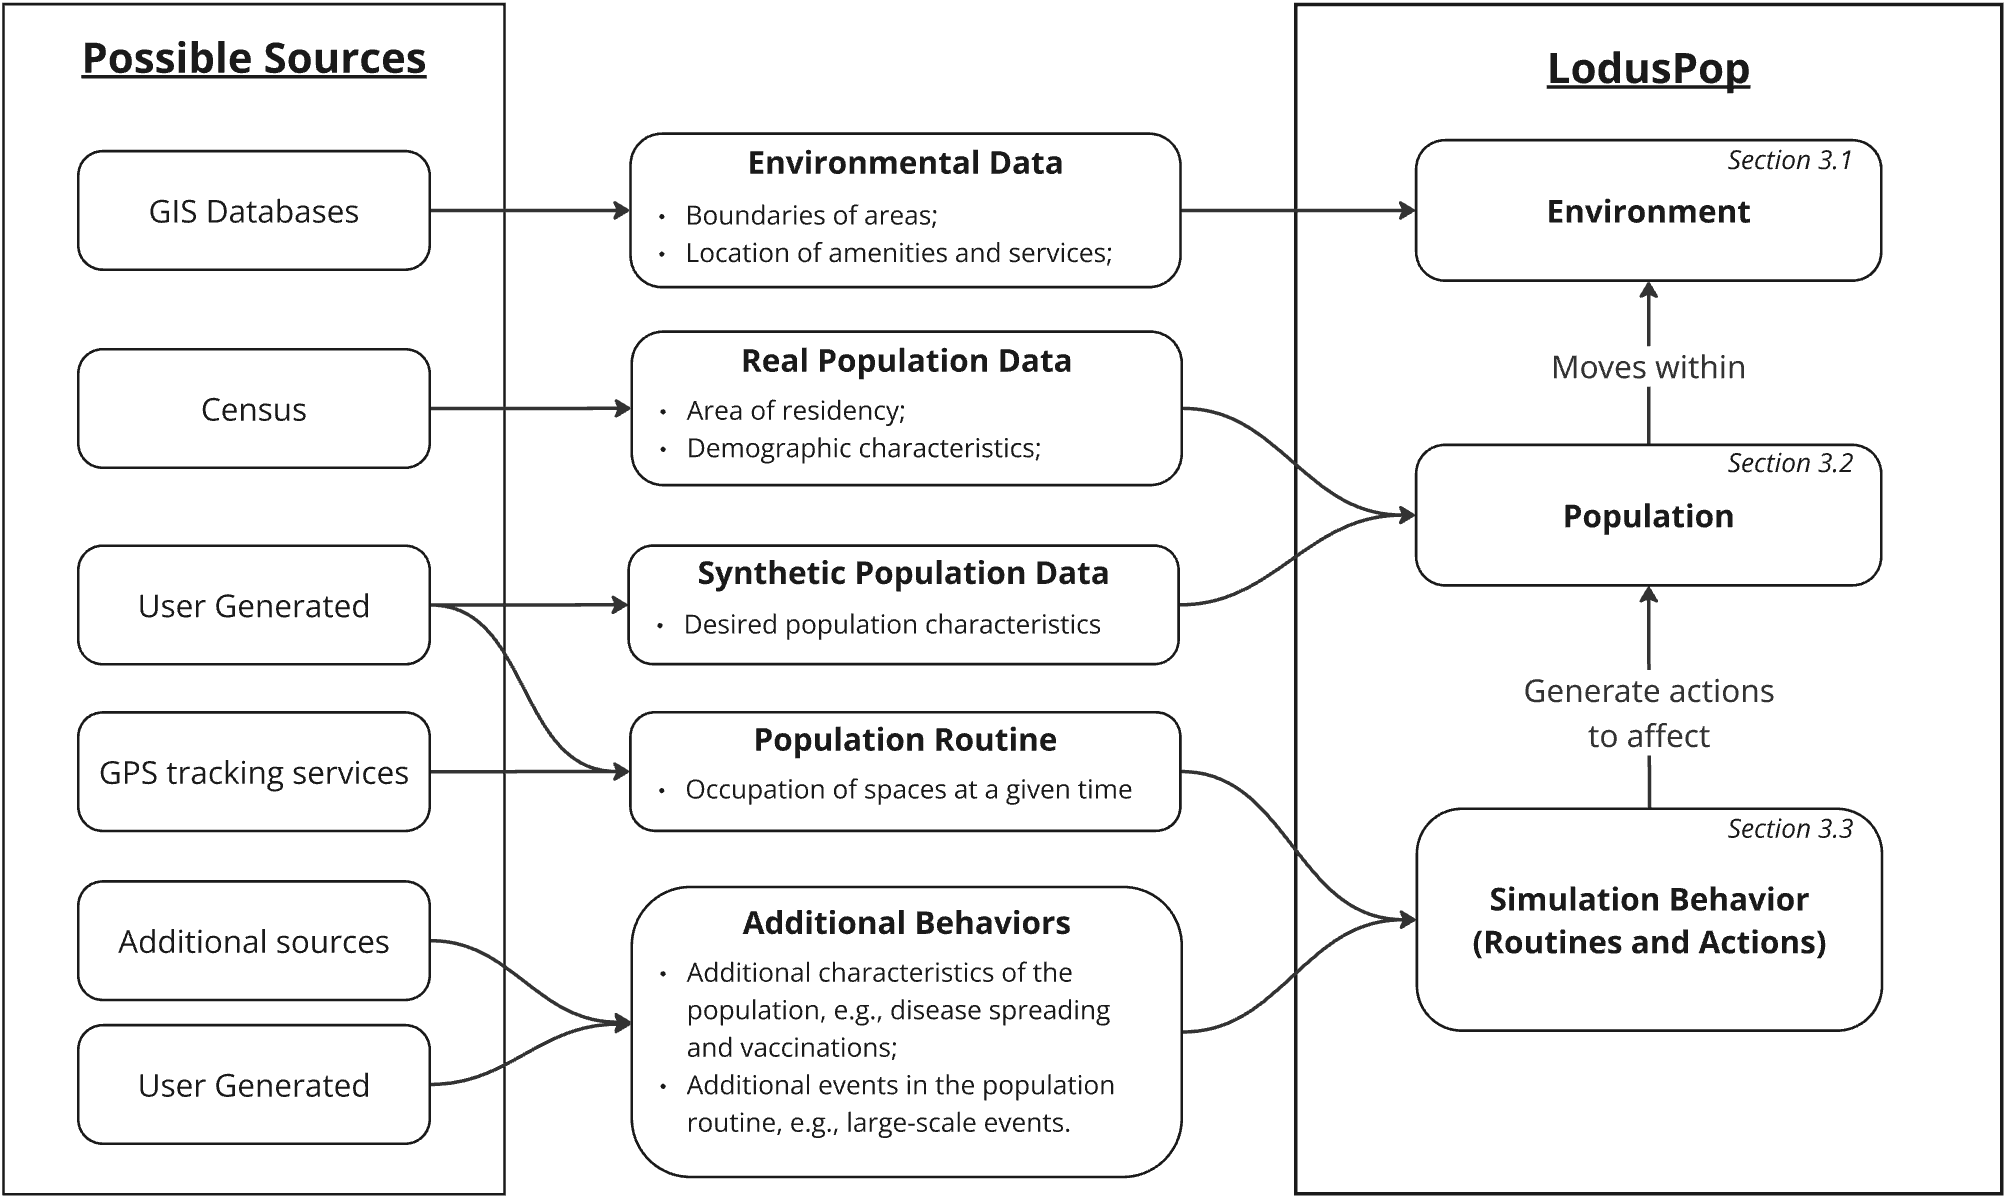
\includegraphics[width=0.98\textwidth]{Figures/DataDiagram3.png}
  \caption{\red{Flowchart illustrating the integration of data sources into the LodusPop framework. Inputs such as GIS databases, census data, user-generated data, and GPS tracking services are processed into geographic data, population characteristics, and behavioral routines. In our proposed model, routines consist of actions that influence population behavior, driving their movement through the environment. %The population and simulation behavior modules are highlighted, as they form the foundation of LodusPop and constitute the core contributions of this work.
  }
  }
  \label{fig:data_diagram}
\end{figure}

%As population mobility frameworks, in general, deal with various size scopes (e.g., neighborhoods, cities, states), we aim to bring crowd simulation strategies to human mobility simulations, in particular the capabilities of abstracting individuality in macroscopic models~\citep{thalmann2007crowd, treuille2006continuum}.
%We propose modeling the population of a simulation as blobs of people (i.e., population groups of varied sizes). In this context, Blob is an abstract structure, similar to a cloud or a legion~\citep{antonitsch2019bioclouds}, but applied to a larger population. 
%In addition, unlike BioClouds and Legion, structures formed by homogeneous populations, our blobs can contain varied individual and group characteristics, evolving in an environment with locations that can request specific population groups.

\red{Population mobility frameworks typically operate across multiple spatial scales, such as neighborhoods, cities, and states. In this work, we seek to integrate strategies from crowd simulation into human mobility modeling, particularly the ability of macroscopic models to abstract individual behaviors~\citep{thalmann2007crowd, treuille2006continuum}. To achieve this, we propose representing populations as blobs—aggregated groups of individuals of varying sizes. In this context, Blob is an abstract structure, similar to a cloud or a legion~\citep{antonitsch2019bioclouds}, but designed to represent larger and more heterogeneous populations. Unlike BioClouds and Legion, which assume homogeneous population clusters, our blobs can encompass diverse individual and group attributes and evolve within environments containing locations that demand specific population profiles.

Furthermore, our environment design builds upon the approach proposed by Silva et al.~\citep{silva2020lodus}. However, our model introduces greater flexibility, allowing regions of the simulated environment to represent different semantic entities beyond the fixed hierarchy of countries, states, regions, and cities, enabling more adaptable and context-specific representations.}

In LodusPop, we can define a set of characteristics for each blob, representing a population of a specific profile distributed in the environment and changing temporally and spatially in the simulation. For instance, one group, representing a blob, might consist of children going to school in the morning and returning home in the afternoon, illustrating spatial movement within a city. Another example involves changes in population parameters, such as healthy workers commuting to their jobs in the morning, with some individuals becoming sick during the day, resulting in healthy individuals returning home and sick individuals heading to a hospital, in this case representing a split in the blob structure.

%This paper focuses on simulating population dynamics within the LODUS environment. However, we do not present all the ideas behind the granularity of the space to provide representation in countries, states, regions, and cities (for further information, please consider~\citep{silva2020lodus}), but only data that is needed to simulate the population movement in the present work.
Our proposed model considers the following elements to provide population simulation, which will be described in the next sections. 
\begin{itemize}
    \item a) An environment modeled as a graph of regions and points of interest that the population can occupy;
    \item b) The population is modeled as blobs that can split and merge and can contain characteristics of the population; and
    \item c) a set of population movement actions and routines to describe the desired population behavior during the simulation.
\end{itemize} 

\subsection{Environment}
\label{sec:environment}

To adequate our population mobility simulation to different spatial scopes, we model the environment as an abstract graph composed of \textit{regions} and \textit{points of interest}. The regions ($R$) represent areas of physical space in the virtual world that can contain points of interest ($P$), which represent locations that motivate human travel and that can have population groups (i.e., blobs $B$). 
When setting up a simulation, users define the spatial scope that $R$ and $P$ represent. For example, in a city simulation, $R$ could correspond to districts, while $P$ might represent markets, malls, hospitals, residential buildings, and commercial centers. 


\redb{A region $R$ is represented as a set of points of interest $\{P_1, ..., P_m\}$. Each point of interest $P_i$ stores the blobs currently located there, denoted $\bm{B}_{P_i}$ and a local routine $Ro_{P_i}$
that specifies which actions occur at that location over time as the simulation evolves (\ref{sec:routines}). Table~\ref{tbl:notation_env} summarizes the notation used for regions and points of interest.} 
Additionally, Appendix~\ref{app:input} outlines the process of defining the input data necessary for designing a simulation. Appendix~\ref{app:input_environment} specifically addresses the data required to model the simulation environment.


%A region $R$ is represented as a set of $P$. In turn, $P$ represents locations that the population can occupy as they move during a simulation. A certain $P_i$ is represented by a tuple $(\bm{B}_{P_i}, Ro_{P_i})$, where $\bm{B}_{P_i}$ is a vector of zero or more population blobs currently located in $P_i$. Each $P_i$ has only one $Ro_{P_i}$, which is a local routine of actions that describes the demand for a population to be at $P_i$ over time as the simulation evolves. 

Indeed, this characterizes an inversion of responsibility compared to what usually happens in population simulations. \redb{In many agent-based approaches, populations decide where to go based on individual preferences or probabilistic rules, requiring granular data about individual movements and locations. Even in field-based models, where motion is guided by environmental potentials or vector fields, agents typically remain the entities that sample and follow these fields.
In our case, the environment is responsible for decision-making regarding the occupation of the population during the simulation, i.e., locations ask for people instead of people choosing where to go. We believe that shifting the focus to the environment as the decision-maker minimizes dependence on granular individual-level data. This shifts part of the decision logic from individuals to points of interest and regions, and is designed to minimize dependence on granular individual-level data by leveraging aggregated or generalized information about population distributions and environmental conditions. }%Instead, it leverages aggregated or generalized information about population distributions and environmental conditions to guide movement.
For example, a $P_m$ representing a market can request consumers, i.e., $P_m$ has a local routine $Ro_{P_m}$, which defines that a certain population of determined characteristics will go to the market during the simulation. $\bm{B}_{P_m}$ represents all the population blobs that are currently on the market.

Other examples in the same region $R$ can be a school that requests students, and hospitals that request patients. In these cases, school is a $P_j$ in $R$, in which $Ro_{P_j}$ is the local routine to go to the school and $\bm{B}_{P_j}$ is a specific population of students. 
\red{Similarly, the hospital is also a $P_k$ in $R$, and $Ro_{P_k}$ is a local routine that should be executed at the hospital.} 
Additionally, $\bm{B}_{P_k}$ is a particular population that goes to the hospital. \red{Figure~\ref{fig1:environment} presents a diagram of a LodusPop environment, representing regions, points of interest, and blobs.}
As humans generally tend to present cyclical behavior in their movement~\citep{gonzalez2008understanding}, repeating similar routines daily or weekly, a LodusPop simulation is also cyclical, where local routines $Ro$ repeat every time cycle of simulation. 
The user defines the temporal scope of a cycle when designing the simulation. A cycle may represent an hour, a day, a month, etc.

\begin{figure}[ht]
 \centering
  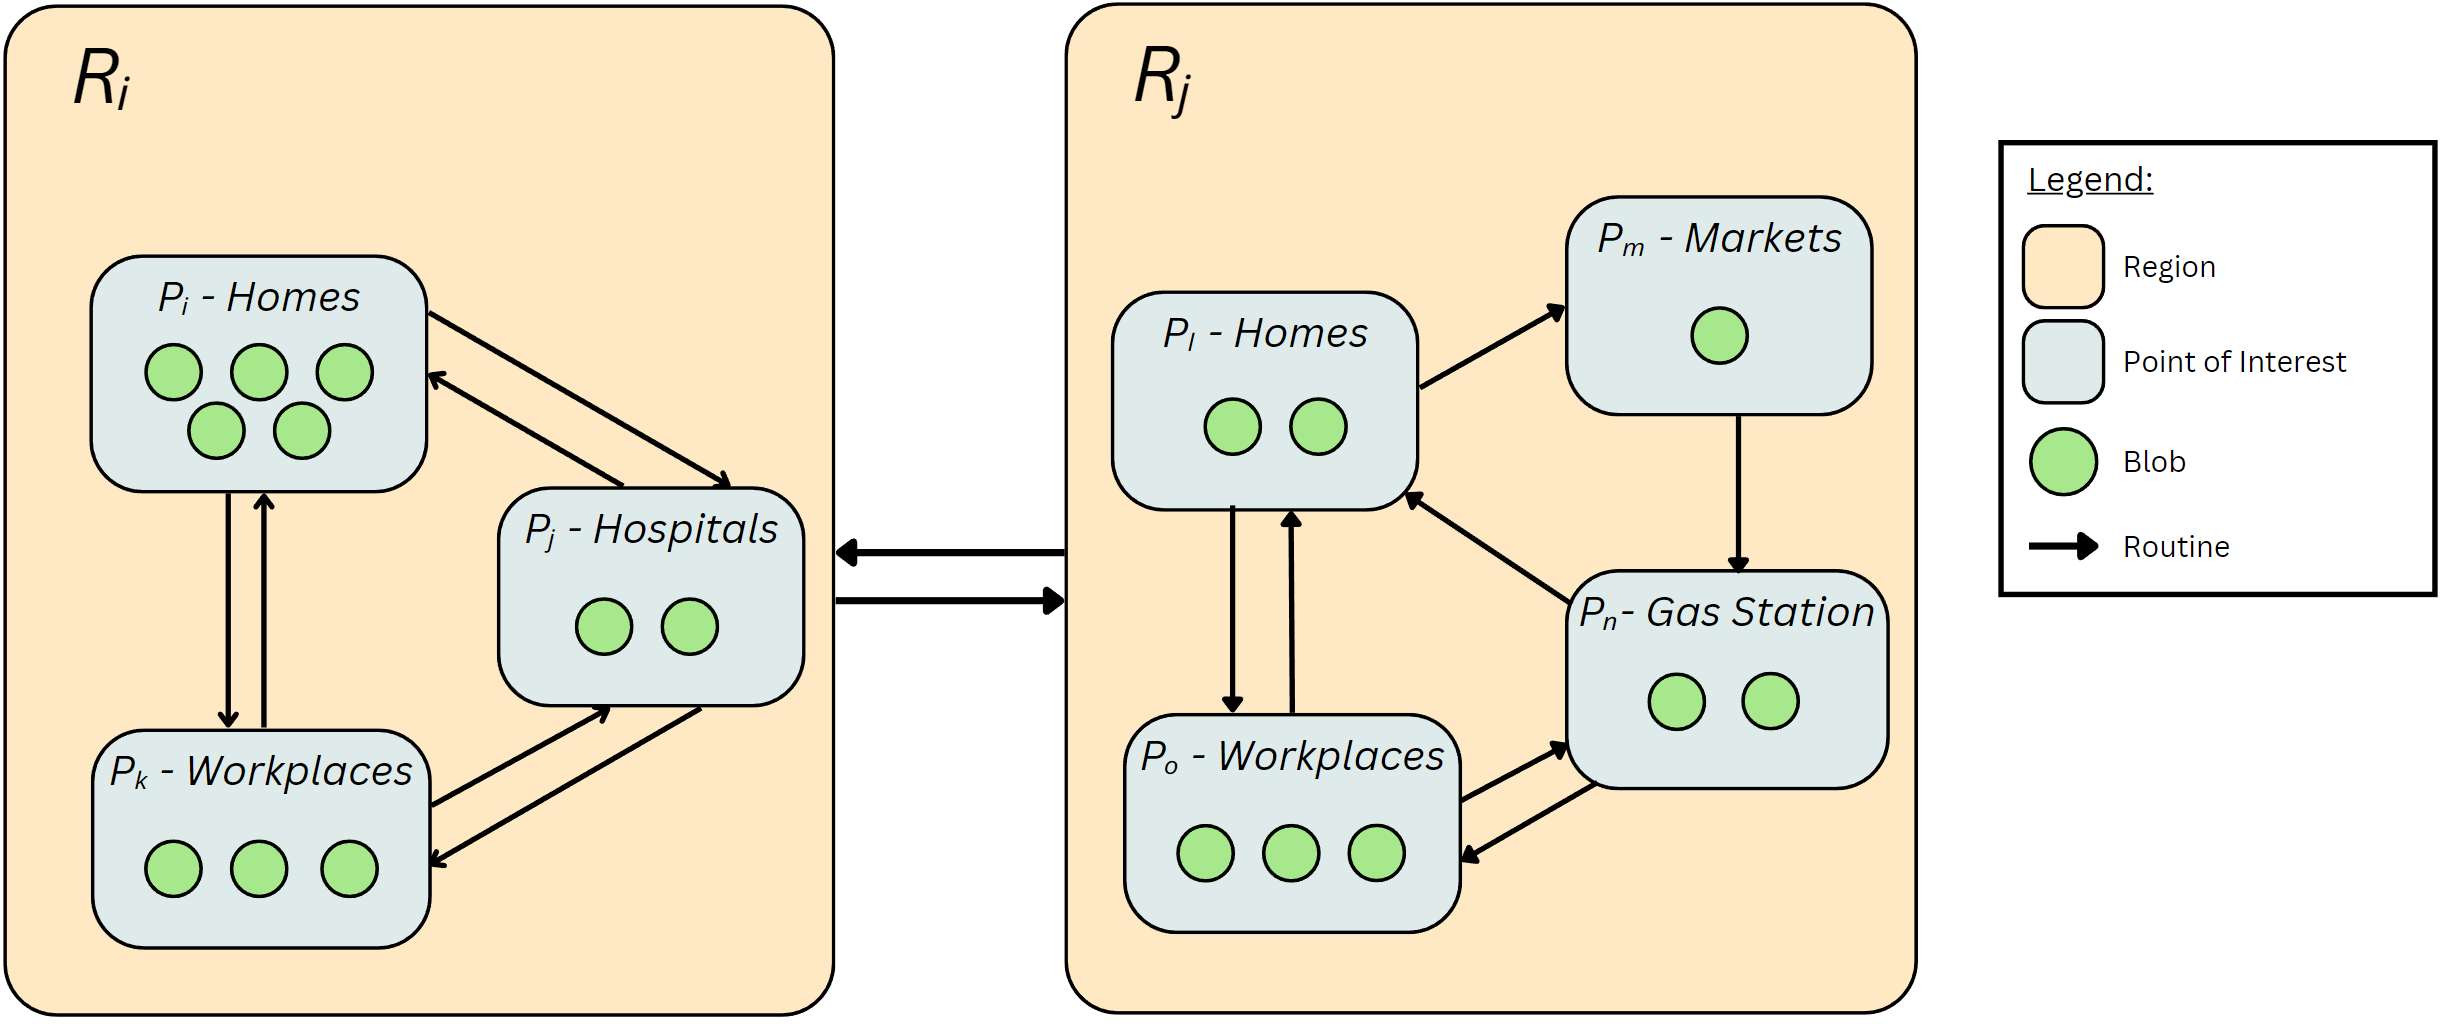
\includegraphics[width=0.98\textwidth]{Figures/Environment.png}
  \caption{\red{A diagram of a LodusPop environment. The figure presents two regions, $R_i$ and $R_j$, containing different points of interest $P$. Each point of interest may contain groups of the population (i.e., blobs), and routines are responsible for moving them in the environment during the simulation.}} 
  \label{fig1:environment}
\end{figure}

\begin{table}[h]
\redb{
\footnotesize
\centering
\caption{Mathematical notation and descriptions of the elements defined in Section~\ref{sec:environment}.}
\label{tbl:notation_env}
\begin{tabularx}{\linewidth}{@{}lcX@{}}
\toprule
\textbf{Element} & \textbf{Notation} & \multicolumn{1}{c}{\textbf{Description}} \\ \midrule
Region                                                             & $R$        & Represent areas of physical space in the virtual world that can contain points of interest. A region $R_i$ is defined as a set of $P$.  \\ \midrule
\begin{tabular}[c]{@{}l@{}}Point of\\ Interest\end{tabular}        & $P$        & Represent locations that the population can occupy as they move during a simulation. A $P_i$ is defined by a collection of population blobs ($\bm{B}_{P_i}$) and its local routine ($Ro_{P_i}$)  \\  \bottomrule
\end{tabularx}
} %end of \redb
\end{table}


\subsection{Population}
\label{sec:population}
%The population in LodusPop is represented by the abstraction of people as already defined blobs $B$, always located in some point of interest.
The population in LodusPop is represented by an abstraction of people into blobs $B$, each always located at some point of interest. These blobs describe the population in groups rather than tracking individuals.
\redb{
%A blob represents a group of individuals that share the same traceable and sampled characteristics at a given point of interest. 
Formally, we denote a blob as $B = (TP, \bm{Tc}, \bm{Sc})$ where $TP$ is the total number of individuals in the blob, $\bm{Tc}$ is the collection of traceable characteristics, and $\bm{Sc})$ is the collection of sampled characteristics. Table~\ref{tbl:notation_pop} summarizes this notation and the associated terminology.

We distinguish two types of characteristics. \textit{Sampled Characteristics}, collected in $\bm{S_c}$, are attributes represented by their distribution within the blob. For example, a sampled characteristic \textit{Age} may have categories \textit{Child}, \textit{Adult} and \textit{Elder}, each associated with a certain number of individuals. By combining multiple sampled characteristics, we can jointly describe attributes such as age, level of schooling and employment status.
\textit{Traceable Characteristics}, collected in $\bm{T_c}$, are attributes whose values are explicitly stored as a single value for the entire blob, rather than as a distribution over categories. For instance, a traceable characteristic \textit{Vaccination status} with values \textit{Vaccinated} and \textit{Unvaccinated} implies that each blob in the simulation is composed entirely of vaccinated or entirely of unvaccinated individuals.
}

These characteristics allow us to specify the population in more detail, e.g., elderly people who are currently vaccinated against a given disease or the number of adults who commute to work by bus. Following the previous examples, it becomes possible to track vaccination by age group in the simulation by identifying all blobs $B$ with a \textit{Vaccinated} status and their respective \textit{Age} distributions. Figure~\ref{fig2:blob_diagram} shows a diagram of a blob, including its characteristics and associated distributions. Appendix~\ref{app:input_population} presents an example of the input data required to model the initial population in simulations.

%A blob $B$ is represented as a set of attributes that describe the population to be simulated. For example, an attribute representing the characteristic \textit{Age} may have \textit{Child}, \textit{Adult}, and \textit{Elder} as possible categories (or values), each associated with a certain number of people. Using a collection of attributes, the population can be modeled with multiple characteristics, such as age, level of schooling, and employment status. These attributes are referred to as \textit{Sampled Characteristics}, and all blobs $B$ must have at least one of them.
%Blobs can also have a second set of characteristics, named \textit{Traceable Characteristics}, modeled as pairs of values instead of categories. For example, we can model a \textit{Vaccination Status} characteristic with the possible values: \textit{Vaccinated} and \textit{Unvaccinated}, so each blob in the simulation will be composed of people who are either all vaccinated or all unvaccinated. Sampled and traceable characteristics can be created to specify better a population, e.g., elderly people who are currently vaccinated against a given disease or the number of adults who go to work by bus. 
%Following the previous examples, it becomes possible to track vaccination per age group in the simulation by identifying all blobs $B$ with a \textit{Vaccinated} status and their respective \textit{Age} distribution. \redb{Table~\ref{tbl:notation_pop} lists the mathematical notation and descriptions of the elements introduced in this section.}




%Detailing the blob $B_i$, it is defined as a tuple $(TP_i, \bm{Tc}_i, \bm{Sc}_i)$, where $TP_i$ is the total population size (scalar value), $\bm{Tc}_i$ is a vector of traceable characteristics (pairs of values), and $\bm{Sc}_i$ is a vector of sampled characteristics.
%Each traceable characteristic $j$ in $\bm{Tc}_i$ is composed of an identifier (i.e., a string) and its value (not restricted by type).
%Each sampled characteristic $k$ in $\bm{Sc}_i$ is also a tuple $(N_k, \bm{D}_k)$, where $N_k$ is the string identifier of this characteristic (e.g., age or occupation), and $\bm{D}_k$ is the vector that contains the categories of the population in that given characteristic. 
%A sample characteristic may contain any number of labeled scalar values, e.g., \textit{age} represented as the labels \textit{children}, \textit{adults} and \textit{elders}, having respectively 20, 40, and 10 individuals. The sum of populations at each distribution in $\bm{Sc}_i$ must equal the total population $TP_i$ which is part of blob definition. 
%Figure~\ref{fig2:blob_diagram} contains a diagram of a blob, representing its characteristics, and containing distributions.
%Appendix~\ref{app:input_population} presents an example of the input data required to model the initial population in simulations.


As mentioned before, during the simulation, blobs in $P_i$ are affected by the local routine $Ro_{P_i}$.
Routines can select a specific population profile to be affected, e.g., moving only children to school, i.e., people from a particular sample attribute ``Age'' in the category ``child'' should go from $P_i$ to $P_j$.
This type of operation in the population $B_i$ of a certain $P$ uses a population template. 

\redb{A population template $T$ specifies which individuals are affected by an action and in what quantity. We represent it as $T = (T_Q, \bm{T_{Tc}}, \bm{T_{Sc}})$, which specifies i) the quantity of people to be affected, ii) an optional a set of predicates on traceable characteristics, and iii) is an optional set of predicates and distributions on sampled characteristics. When applied to a set of blobs, a template behaves as a filter that identifies the subset of individuals that satisfy all predicates and are counted towards $T_Q$.}
%where $T_Q$ is the quantity of people to be affected (for example, an absolute number or a fraction of the eligible population), 
%$\bm{T_{Tc}}$ is an optional a set of predicates on traceable characteristics, and  $\bm{T_{Sc}}$ is an optional set of predicates and distributions on sampled characteristics. When applied to a set of blobs, a template behaves as a filter that identifies the subset of individuals that satisfy all predicates and are counted towards $T_Q$. }
%A blob $B_i$ is only affected by the template $T$ if its traceable or sampled properties are specified in $T$. Indeed, $T$ operates as a filter to select a population from $B$.

\begin{figure}[ht]
 \centering
  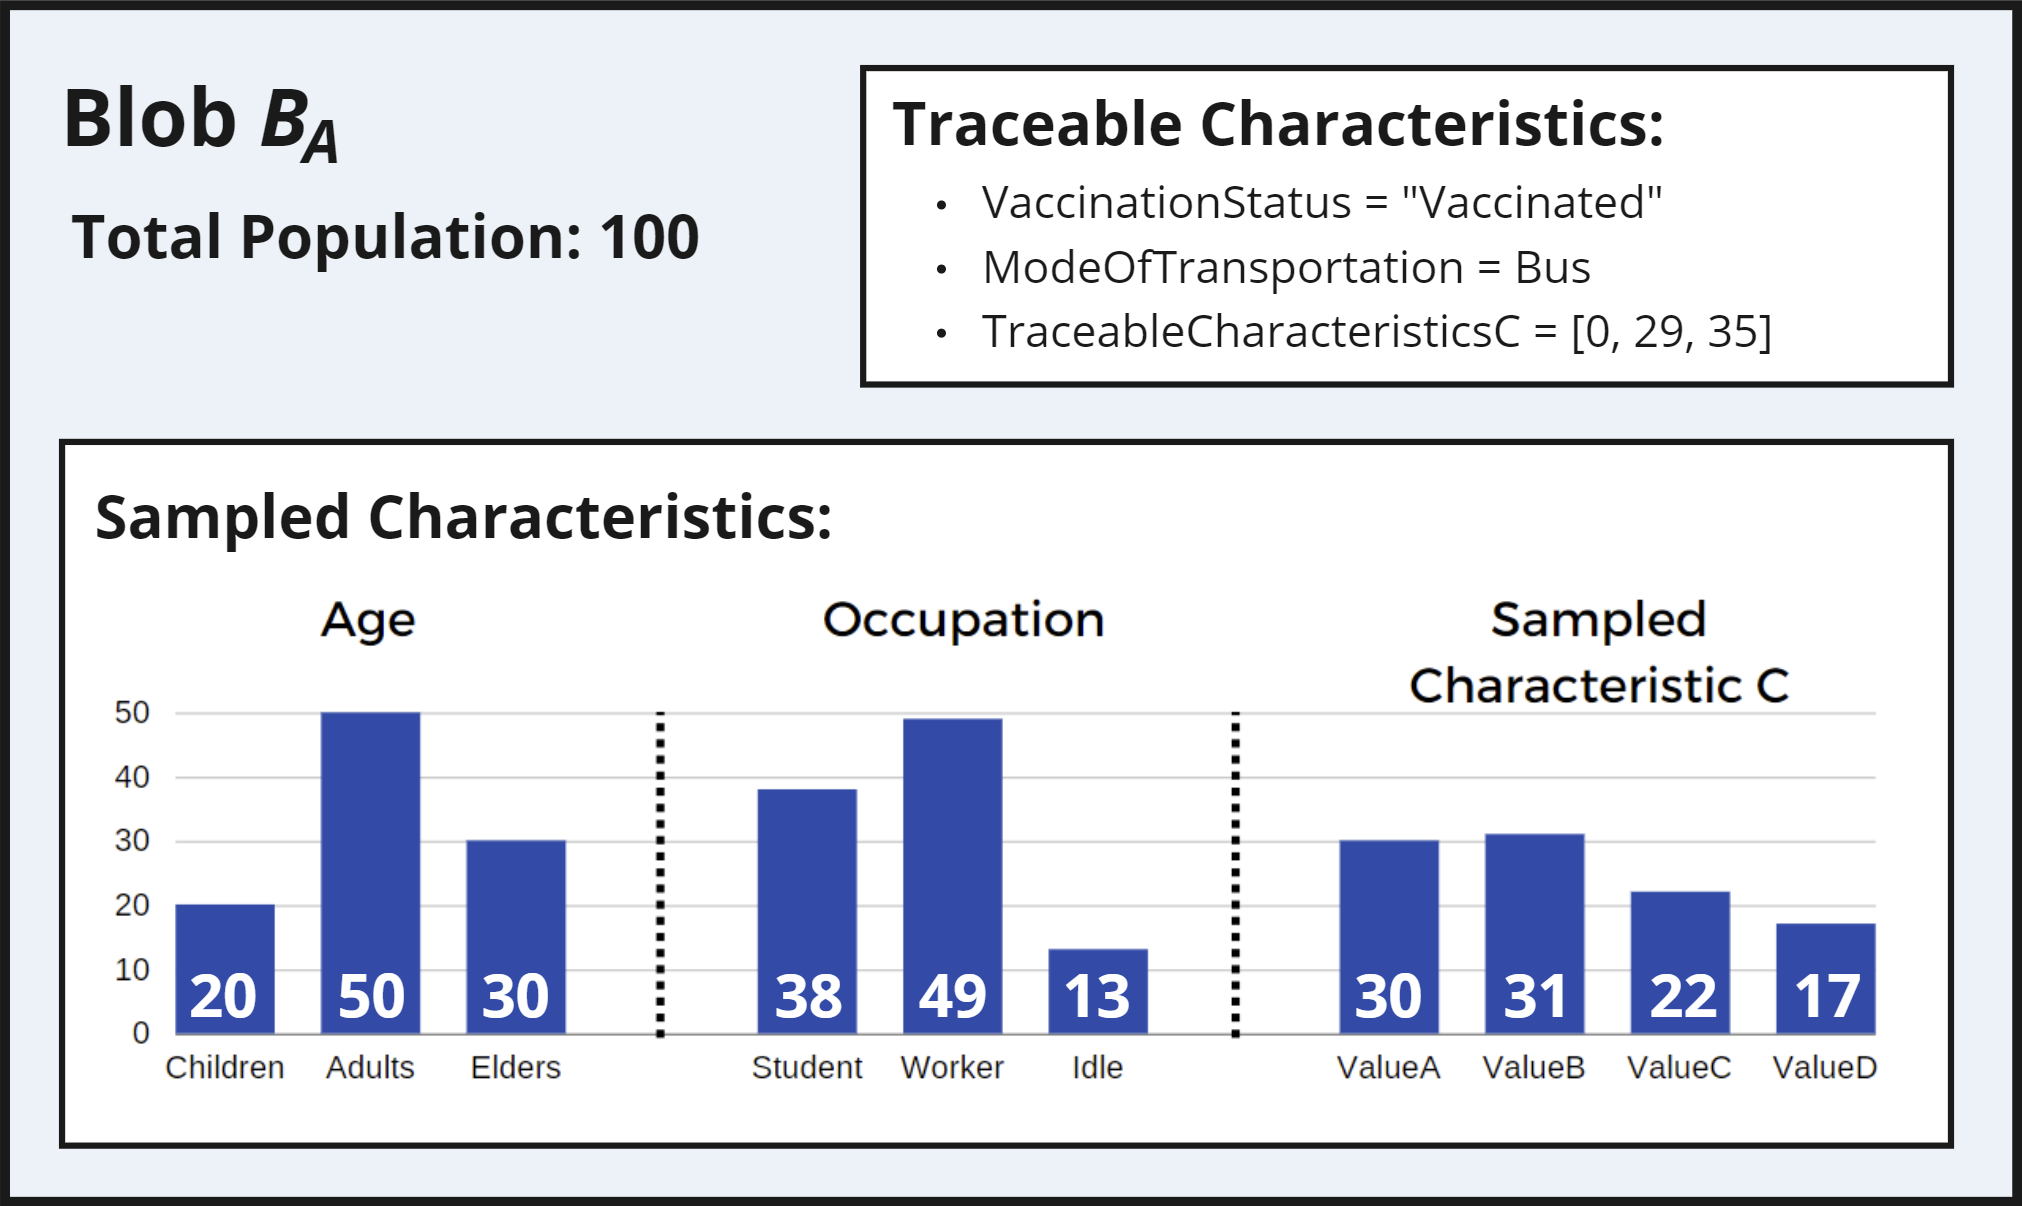
\includegraphics[width=0.9\textwidth]{Figures/BlobDiagram.png}
  \caption{Diagram of a Blob $B_A$ containing 100 people, three traceable characteristics, and three sampled characteristics. Traceable characteristics describe the entire blob population and can have any value type. The distribution of each sampled characteristic sum should be equal to the total population of the blob.} 
  \label{fig2:blob_diagram}
\end{figure}

Consider a blob $B_j$ with two sampled characteristics: \textit{i)} \textit{Age}, which includes the possible values \textit{Children}, \textit{Adults}, and \textit{Elders}, and \textit{ii)} \textit{Occupation}, with possible values \textit{Student} and \textit{Worker}. A template $T$ that specifies \textit{Age=Adults} in its collection of sampled characteristics will target only the specified group within $B_j$, in this case, only adults. If the template $T$ does not include a filter for the second sampled characteristic (Occupation), all occupation categories in $B_j$ are affected. The number of affected individuals in categories such as Students and Workers is determined proportionally based on their distribution within $B_j$. For instance, if $B_j$  contains more students than workers, a larger proportion of students will be selected. This process continues until the total number of individuals defined in $T$ is selected or until there are no remaining eligible individuals in $B_j$.

% Splits
When a blob is operated using a population template $T$, it is possible that only a portion of its population may be affected, e.g., a blob $B_i$ that has 75 people and only 20 are selected in $T$. If the operation is to move to another $P$, then such 20 people will create a new blob. This operation generates a split, i.e., the original blob will be separated into two smaller ones. 
In such an example, a template with quantity $T_Q = 20$ selects 20 people from $B_i$ and splits it by creating a new blob $B_j$, which is moved to a different $P$. 
The same occurs when modifying a blob's $\bm{Tc}$s. For example, another blob $B_k$ has 90 \textit{Healthy} people, 
and 20 are selected, using $T$, to be infected by a disease. The split occurs, and a \textit{InfectionStatus} of $B_l$ (newly created blob) is changed to \textit{Infected}.

% Merge
In addition to split operations, blobs can also be merged, combining their total populations $TP$. 
Each sampled characteristic of the resulting blob is the sum of the respective characteristics of the merged blobs. A merge can only occur between blobs currently in the same $P$ and with the same values in all their traceable characteristics. This restraint allows us to merge only populations that share the same traceable features.
% Figure
Figure~\ref{fig3:blob_operations_with_template} presents a diagram of blobs affected by two templates, resulting in splits and merges. The first scenario, depicted at the top of the figure, demonstrates the relocation of a population. %In 1a), the initial blob $B_i$ has a population of 100 located in $P_i$. In 1b), a template $T$ selects 30 individuals, resulting in the split of $B_i$ and the creation of $B_j$. In 1c), $B_j$ is transferred to $P_j$. 
The second scenario illustrates changes in traceable characteristics of a population.% In 2a), two blobs, $B_i$ containing 100 unvaccinated individuals (depicted in red) and $B_j$ containing 50 vaccinated individuals (depicted in green), coexist in $P_i$. In 2b), a template $T$ selects 20 unvaccinated individuals, affecting only $B_i$ and creating $B_k$. In 2c), the traceable characteristic "VaccStatus" of $B_k$ is modified to "Vaccinated." In 2d, $B_k$ is merged with $B_j$ as they now share the same characteristics and exist within the same $P_i$.

\begin{figure}[ht]
 \centering
  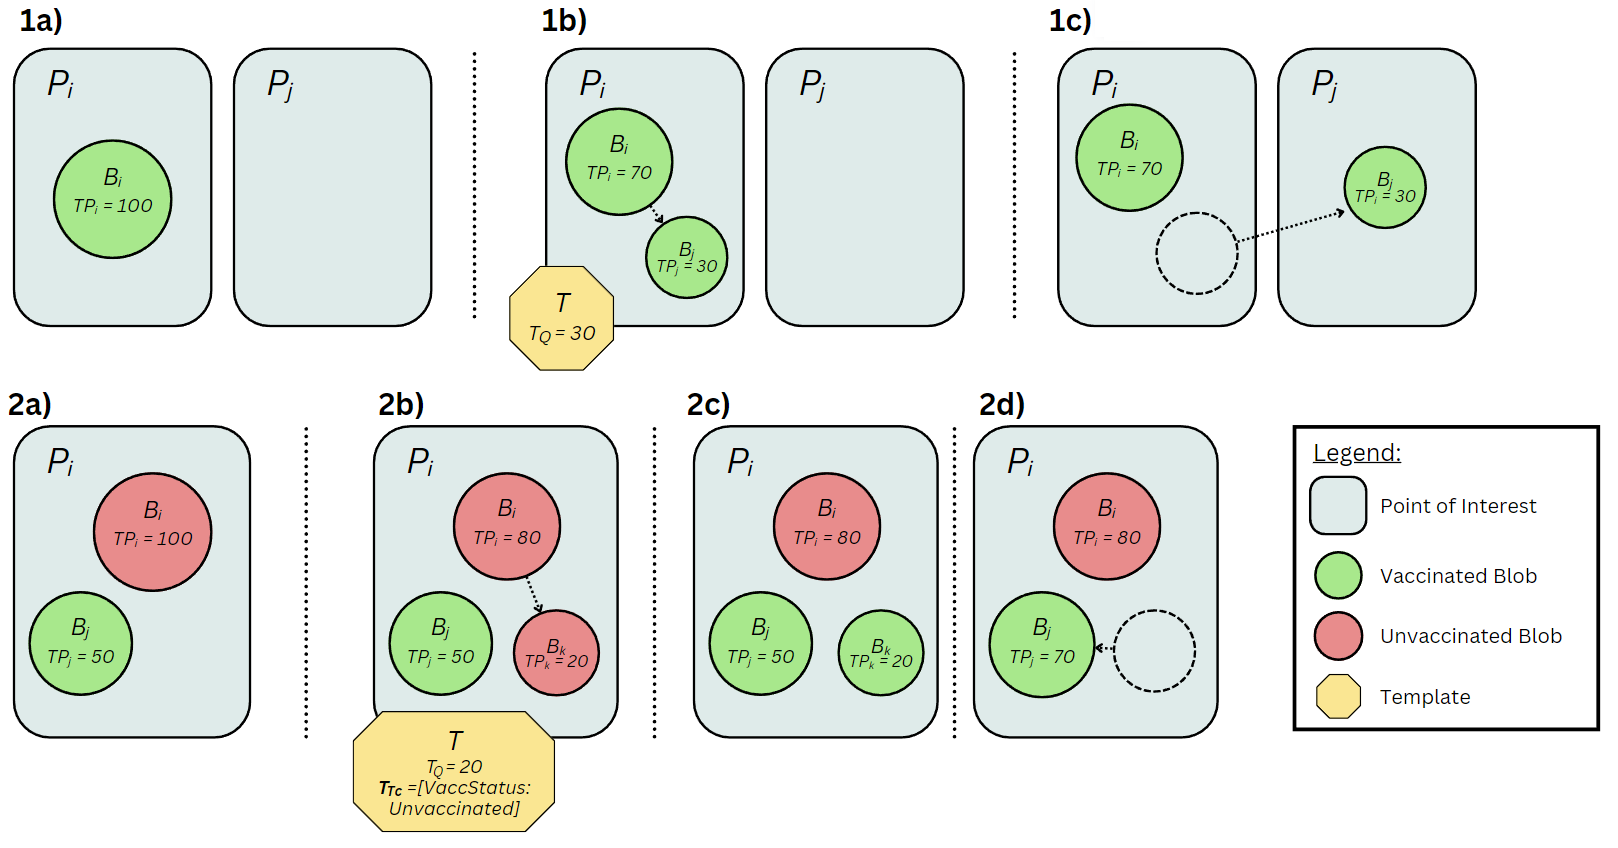
\includegraphics[width=0.99\textwidth]{Figures/BlobOperations.png}
  \caption{
  Diagram presenting two scenarios of blobs being modified. The first scenario (1) (on the top) shows a population being moved to another location. In 1a, the initial blob $B_i$ has a population of 100. In 1b, a template $T$ selects 30 people, splitting $B_i$ and creating $B_j$. In 1c, $B_j$ is moved to $P_j$. The second scenario (2) shows a population's traceable characteristics changed. In 2a, there are two blobs, $B_i$ containing 100 unvaccinated people (in red), and $B_j$ containing 50 vaccinated people (in green). In 2b, a template $T$ selects 20 unvaccinated people, affecting only $B_i$ and splitting it into $B_k$. In 2c, the traceable characteristic \textit{VaccStatus} of $B_k$ is changed to \textit{Vaccinated}. In 2d, $B_k$ is merged into $B_j$ since they now share the same characteristics and are in the same $P_i$.
  } 
  \label{fig3:blob_operations_with_template}
\end{figure}

\begin{table}[h]
\redb{
\footnotesize
\centering
\caption{Mathematical notation and descriptions of the elements defined in Section~\ref{sec:population}.}
\label{tbl:notation_pop}
\begin{tabularx}{\linewidth}{@{}lcX@{}}
\toprule
\textbf{Element}                                                             & \textbf{Notation} & \multicolumn{1}{c}{\textbf{Description}}                                                                                                                                                                                                                                                                                     \\ \midrule
Blob                                                               & $B$        & Represent an abstraction of the population. A $B_i$ is defined as its total population ($TP_i$), a collection of traceable characteristics ($\bm{Tc}_i$), and a collection of sampled characteristics ($\bm{Sc}_i$)                                                                                                         \\ \midrule
\begin{tabular}[c]{@{}l@{}}Traceable\\ Characteristic\end{tabular} & $Tc$       & Characteristic of a blob defined as an identifier (i.e., a string) and its value (not restricted by type).                                                                                                                                                                    \\ \midrule
\begin{tabular}[c]{@{}l@{}}Sampled\\ Characteristic\end{tabular}   & $Sc$       & Characteristic with a categorical distribution over the blob population. Defined as a string identifier and a collection of its possible categories, each associated with a certain number of people.                                                                                                                             \\ \midrule
\begin{tabular}[c]{@{}l@{}}Population\\ Template\end{tabular}      & $T$        & Specifies which individuals are affected by an action and in what quantity, operating as a filter to select a population from a $B$.                 \\ \bottomrule
\end{tabularx}
} %end of \redb
\end{table}

\subsection{Routines and Actions}
\label{sec:routines}

\redb{All behavioral dynamics in LodusPop are driven by routines, which associate discrete time steps with actions that operate on blobs.
We consider a simulation organized into cycles of fixed length 
$d$ steps. Within a cycle, time is indexed by an integer $t \in \{0, ..., d-1\}$, which we refer to as the cycle step. 

A (local or global) routine is a finite set of pairs $R = \{(t, A)\}$, where $t$ is a cycle step and $A$ is an action to be executed at that step.
For each point of interest $Pi$, the local routine is denoted $Ro_i$ and specifies the actions that should be performed by $Pi$.
The Global Routine $GRo$ has the same structure but applies its actions to all points of interest in the environment.

Each action $A$ is defined as $A = (N, T, \bm{V})$, where $N$ is an identifier for the action type (e.g., MOV or CH); $T$ is a population template as defined in Section~\ref{sec:population}, selecting the subset of a blob that will be affected; and $\bm{V}$ is a vector of additional values (parameters) used by the action. 
Table ~\ref{tbl:notation_rout} summarizes the notation introduced in this section.

In the core implementation, LodusPop provides two built-in action types:
\textit{move population} (MOV), which moves a subset of a blob between points of interest; and \textit{change traceable characteristic} (CH), which modifies the traceable characteristics of a subset of a blob.

A MOV action expects its parameter vector $\bm{V}$ to specify an origin and a destination point of interest. For example, the local routine of $P_i$ may include the pair $(t = 15, A)$, where $A = (MOV, T_i, V_i)$, with $T_i=(T_Q=20, T_{Tc}=\emptyset, T_{Sc}=\{Age=Child\})$, and $V_i$ encoding $P_i$ as origin and $P_j$ as destination. At cycle step $t = 15$, this action selects 20 children from the blobs at $P_i$ , splits them into a new blob, and moves that blob to 
$P_j$.

A CH action expects $\bm{V}$ to contain the name of a traceable characteristic and its new value. For instance, the local routine of $P_j$ may include $(t = 25, A')$, with $A' = (CH, T_j, V_j)$, where $T_i=(T_Q=20, T_{Tc}=\{Status=Unvaccinated\}, T_{Sc}=\emptyset)$, and $\bm{V_j}$ encodes the update ``Status := Vaccinated''. At cycle step $t=25$, this action selects 20 unvaccinated individuals from the blobs at $P_j$, splits them into a new blob, and changes the traceable characteristic Status of that blob to Vaccinated. Figure~\ref{fig3:blob_operations_with_template} illustrates both the movement and characteristic-change scenarios.

}

%Routines model the repeating temporal behavior of population $B$ located in any given $P$. The local routine of $P_i$ is defined as $Ro_{P_i}\xrightarrow{}\{t,A_i\}^\ast$, where $t$ is the time in the simulation that action $A_i$ should be performed. A given action $A_i$ is defined as a tuple $(N_{i}, T_{i}, \bm{V}_{i})$, where $N_{i}$ is an identifier for the action type, $T_{i}$ is a population template describing the profile and quantity of people being affected (as described in the last section), and $\bm{V}_{i}$ is a collection of values that can be used in action.

%LodusPop contains two types of actions: \textit{move population} (MOV), and \textit{change traceable characteristic} (CH).
%The \textit{move population} action type is responsible for moving a group of people in the environment and must receive the origin and destination of the movement, i.e., $P_i$ and $P_j$, respectively.
%For example: $Ro_{P_i}=\{15, \{MOV, T_i=\{20, \{\},\{age=child\}\}, P_j\}\}$, i.e., at time 15 of the simulation, 20 people from $B_i$ located at $P_i$ will move to $P_j$.
%The \textit{change traceable characteristic} action type is responsible for modifying the $\bm{Tc}$s of blobs. It must receive the identifier of the traceable characteristic being changed and its new value. One example is following described:  $Ro_{P_j}=\{25, \{CH, T_j=\{20,\{status=unvaccinated\}, \{\}\}, status=vaccinated\}\}$, i.e., at time 25 of simulation, 20 people from $B_j$ located at $P_j$ will change this status of vaccination. Figure~\ref{fig3:blob_operations_with_template} presents a diagram of blobs affected by the two detailed actions. The first scenario represents a \textit{move population} action, where a blob is moved from $P_i$ to $P_j$, and the second scenario presents a \textit{change traceable characteristic} action.

% Global routines and Queueing
The same action representation is used by the Global Routine $GRo$. For example, a MOV or CH entry in $GRo$ is executed at the specified cycle step 
$t$ for all points of interest simultaneously, enabling the modeling of global phenomena such as random walks or disease spread. Appendix~\ref{app:input_routine} provides an example of the input data used to encode both local routines and the Global Routine.

%LodusPop is also an additional resource for modeling the global behavior of a simulation.The Global Routine can be used to model global events, e.g., random walks and the spread of diseases.The Global Routine is defined as $GRo\xrightarrow{}\{t,A\}^\ast$, where $t$ is the time in the simulation that action $A$ is performed by all $P$s in the environment. Appendix~\ref{app:input_routine} presents an example of the input data required to model a Global Routine ($GRo$) and the local routines for specific points of interest.

% New action types with Plugins
New action types can be added via plugins. A plugin registers an additional identifier $N$ together with a function that consumes actions of that type. Plugin actions retain the same structure $A=(N,T,V)$. The simulation still uses the population template $T$ to select the affected individuals and passes $T$ and $\bm{V}$ to the plugin’s function. Appendix~\ref{app:plugin} illustrates how plugins can be used to introduce custom action types into simulations.

%New action types can be included in the simulator using plugins. A plugin can add another action type and a function to consume it. Actions included by plugins have the exact definition as previously described. Considering a new action $A_j$, the system is responsible for matching the identifier for the action type $N_{A_j}$ with the function that should consume it, sending the population template $T_{j}$ and additional values $\bm{V}_{j}$ as parameters the function. Appendix~\ref{app:plugin} provides an example of how plugins can be used to introduce new action types into simulations.

To achieve repeating temporal behavior, the simulation iterates over cycle steps $t = 0, ..., d-1$ within each cycle. At the beginning of each step 
$t$, the simulator collects all actions $(t,A)$ from $GRo$ and from every local routine. For each action, it:
\begin{enumerate}
    \item uses the template $T$ to select the affected population from the current blobs;
    \item applies the action semantics (e.g., move or characteristic change), which may split existing blobs or create new ones; and
    \item performs, at the end of the step, a merge operation at each point of interest, combining blobs that share identical traceable characteristics.
\end{enumerate}

Figure~\ref{fig:simulation_diagram} illustrates the simulation behavior over a single cycle. Appendix~\ref{app:simulator} presents an example of a simulation script that manages the overall control of the simulation flow. \redb{In the current implementation, actions scheduled for the same cycle step are executed sequentially in the order in which they are listed in the input, and we apply the same ordering to actions in the global routine $GRo$. 
Each action is treated as an atomic operation: it selects a population according to its template based on the current blob configuration, applies the corresponding modifications, and immediately updates the state before the next action is evaluated. As a consequence, the same blob (or its descendants) may be affected by multiple actions within a single cycle step, but the later actions always see the state resulting from earlier ones in that step.}


%To achieve a repeating temporal behavior for $P$s, the simulation execution comprises cycles that repeat every $d$ step, with each step named a \textit{cycle step}.
%The simulation designer can define the temporal scope of a simulation by specifying the semantics of a cycle step and the total cycle duration $d$. For instance, a cycle with $d = 24$ could represent a 24-hour day, where each cycle step corresponds to one hour, or a two-year period, where each step represents a month.
%For a given point of interest $P_k$, all actions in its local routine $Ro_{P_k} \xrightarrow{}\{t,A\}^\ast$ are executed once per cycle, where $t$ denotes the cycle step at which an action $A$ is performed. The same principle applies to the global routine $GRo$.
%Appendix~\ref{app:simulator} presents an example of a simulation script that manages the overall control of the simulation flow.

%Figure~\ref{fig:simulation_diagram} illustrates the simulation behavior process. \redb{In the current implementation, actions scheduled for the same cycle step are executed sequentially. For each point of interest $P_k$, we process all actions in its local routine $Ro_{P_k}$ in the order in which they are listed in the input, and we apply the same ordering to actions in the global routine $GRo$. 
%Each action is treated as an atomic operation: it selects a population according to its template $T$ based on the current blob configuration, applies the corresponding move or characteristic change (possibly splitting blobs), and immediately updates the state before the next action is evaluated.
%As a consequence, the same blob (or its descendants) may be affected by multiple actions within a single cycle step, but the later actions always see the state resulting from earlier ones in that step. After all actions at a given cycle step have been processed,} each point of interest examines its blobs in $\bm{B}_{P}$ for potential merging, combining blobs that share identical values for all traceable characteristics.


%Figure~\ref{fig:simulation_diagram} illustrates the simulation behavior process. At the start of each cycle step $t$, all actions scheduled for execution at that step are identified from the Global Routine ($GRo$) and the Local Routines of each $P$. For each action, the affected population is selected based on their template. Subsequently, each blob is modified according to the action type. These updates may result in the blob splitting, such as moving a subset of the population to a new point of interest or altering the characteristics of a portion of the blob (as shown in Figure~\ref{fig3:blob_operations_with_template}). Finally, each point of interest examines its blobs in $\bm{B}_{P}$ for potential merging, combining blobs that share identical values for all traceable characteristics.


\begin{figure}[ht]
 \centering
  
\includegraphics[width=0.99\textwidth]{Figures/SimulationBehaviorDiagram.png}
  \caption{Diagram of the simulation behavior, illustrating the identification and execution of actions from global and local routines. 
  \redb{At each cycle step, all actions scheduled for that step are collected and executed sequentially in the order defined by the simulation input. Each action modifies blobs by moving them or changing their traceable characteristics and may cause splits; subsequent actions in the same step operate on this updated state.} At the end of the step, blobs with identical traceable characteristics in the same point of interest are merged.} 
  \label{fig:simulation_diagram}
\end{figure}



\begin{table}[h]
\redb{
\footnotesize
\centering
\caption{Mathematical notation and descriptions of the elements defined in Section~\ref{sec:routines}.}
\label{tbl:notation_rout}
\begin{tabularx}{\linewidth}{@{}lcX@{}}
\toprule
\textbf{Element}                                                             & \textbf{Notation} & \multicolumn{1}{c}{\textbf{Description}} \\ \midrule
\begin{tabular}[c]{@{}l@{}}Local\\ Routine\end{tabular}            & $Ro$       & Model the repeating temporal behavior of a population $B$ located in any given $P$. It is defined as $\{t,A_i\}^\ast$, where $t$ is the time in the simulation that action $A_i$ should be performed.                                                                                                               \\ \midrule
\begin{tabular}[c]{@{}l@{}}Global\\ Routine\end{tabular}           & $GRo$      & Modeling the global behavior of a simulation. Similar to a Local Routine, but it is applied to all $P$s in the simulation                                                                                                                                                                                           \\ \midrule
Action                                                             & $A$        & Represents an action to be performed in the population, either moving or changing its characteristics. A $A_i$ is defined as an identifier for the action type ($(N_{i}$), a population template to select the population to be affected ($T_{i}$), and a collection of values to be used by the action ($\bm{V}_{i})$. \\ \bottomrule
\end{tabularx}
} %end of \redb
\end{table}

% Tabela completa
%Table~\ref{tbl:notation} provides an overview of the mathematical notation and descriptions for elements presented in this section, e.g., a region ($R$) and a point of interest ($P$). The table serves as a reference for the key elements and their definitions.

\begin{comment}
    

\begin{table}[h]
\redb{
\footnotesize
\centering
\caption{Mathematical notation and descriptions of the elements defined in Section~\ref{sec:proposed_model}.}
\label{tbl:notation}
\begin{tabularx}{\linewidth}{@{}lcX@{}}
\toprule
\textbf{Element}                                                             & \textbf{Notation} & \multicolumn{1}{c}{\textbf{Description}}                                                                                                                                                                                                                                                                                     \\ \midrule
Region                                                             & $R$        & Represent areas of physical space in the virtual world that can contain points of interest. A region $R_i$ is defined as a set of $P$.                                                                                                                                                                              \\ \midrule
\begin{tabular}[c]{@{}l@{}}Point of\\ Interest\end{tabular}        & $P$        & Represent locations that the population can occupy as they move during a simulation. A $P_i$ is defined by a vector of population blobs ($\bm{B}_{P_i}$) and its local routine ($Ro_{P_i}$)                                                                                                                         \\ \midrule
Blob                                                               & $B$        & Represent an abstraction of the population. A $B_i$ is defined as its total population ($TP_i$), a vector of traceable characteristics ($\bm{Tc}_i$), and a vector of sampled characteristics ($\bm{Sc}_i$)                                                                                                         \\ \midrule
\begin{tabular}[c]{@{}l@{}}Traceable\\ Characteristic\end{tabular} & $Tc$       & Represents a characteristic of the population in a blob. It is defined as an identifier (i.e., a string) and its value (not restricted by type).                                                                                                                                                                    \\ \midrule
\begin{tabular}[c]{@{}l@{}}Sampled\\ Characteristic\end{tabular}   & $Sc$       & Represents a characteristic of the population in a blob. It is defined as a string identifier and a vector of its possible categories, each associated with a certain number of people.                                                                                                                             \\ \midrule
\begin{tabular}[c]{@{}l@{}}Population\\ Template\end{tabular}      & $T$        & Operates as a filter to select a population profile from a $B$. A $T$ is defined as the number of people being affected by the operation ($T_Q$), a vector of traceable characteristics ($\bm{T_{Tc}}$), and a vector of sampled characteristics ($\bm{T_{Sc}}$)                \\ \midrule
\begin{tabular}[c]{@{}l@{}}Local\\ Routine\end{tabular}            & $Ro$       & Model the repeating temporal behavior of a population $B$ located in any given $P$. It is defined as $\{t,A_i\}^\ast$, where $t$ is the time in the simulation that action $A_i$ should be performed.                                                                                                               \\ \midrule
\begin{tabular}[c]{@{}l@{}}Global\\ Routine\end{tabular}           & $GRo$      & Modeling the global behavior of a simulation. Similar to a Local Routine, but it is applied to all $P$s in the simulation                                                                                                                                                                                           \\ \midrule
Action                                                             & $A$        & Represents an action to be performed in the population, either moving or changing its characteristics. A $A_i$ is defined as an identifier for the action type ($(N_{i}$), a population template to select the population to be affected ($T_{i}$), and a vector of values to be used by the action ($\bm{V}_{i})$. \\ \bottomrule
\end{tabularx}
} %end of \redb
\end{table}
\end{comment}

\section{Experimental Results}
\label{sec:results}


This section presents a series of experiments designed to evaluate the key aspects and capabilities of our proposed model, LodusPop. These experiments demonstrate the model's versatility and effectiveness in simulating population dynamics under various scenarios, highlighting its ability to manage complex interactions between the environment and the population. Each experiment highlights specific features of the model:
\begin{enumerate}
    \item \textbf{Random walk behavior} simulates daily routines based on the population's profile (i.e., sampled characteristics) and the proximity of points of interest. For instance, students can be modeled to attend schools during the day, while adults visit nearby pharmacies or supermarkets (Section~\ref{sec:random_walk});
    \item \textbf{Large-scale events} illustrate how disruptions to daily routines impact mobility and how multiple events can compete for the available population  (Section~\ref{sec:large_scale});
    \item \textbf{Infectious disease simulation and vaccination scenarios} model population behavior over extended periods, illustrating how traceable characteristics evolve and how the spread of a disease impacts the population. These scenarios also enable the analysis of dynamic population attributes, demonstrating how public health policies, such as vaccinations or lockdowns, influence disease transmission and population behavior (Section~\ref{sec:contagion}).
\end{enumerate}

All experiments extend the basic functionalities of LodusPop by incorporating plugins that introduce additional action types and traceable characteristics, enabling precise tracking of population evolution throughout the simulations.
%Additionally, these experiments demonstrate the model’s capability to represent populations as abstract blobs of varying sizes, capturing both macro-level and micro-level behaviors. 
\redb{Additionally, these experiments demonstrate the model’s capability to represent populations as abstract blobs of varying sizes, from coarse city-wide aggregates down to blobs that represent very small groups or even single individuals. Macro-scale dynamics are evident when large groups participate in large-scale events across the environment, resulting in changes to mobility patterns (Section~\ref{sec:large_scale}), while finer-grained effects appear when a small subset of the population at a specific location is affected, such as during a disease outbreak (Section~\ref{sec:contagion}).}
%Macro-level dynamics are evident when large groups participate in large-scale events across the environment, resulting in changes to mobility patterns (Section~\ref{sec:large_scale}). On the other hand, micro-level behaviors emerge when a single individual at a specific location is affected, such as during a disease outbreak (Section~\ref{sec:contagion}).
The blob sizes are dynamically adjusted during simulations, ranging from entire neighborhood populations to single individuals. 
Together, these case studies validate the model’s performance and highlight its potential for practical applications in urban planning and public health.

\subsection{Case-Scenario: Porto Alegre, Brazil}
\label{sec:case_scenario}

LodusPop, designed to work with real-world data, was tested to model the population behavior of Porto Alegre, Brazil. Following our proposed definitions for the environment (Section~\ref{sec:environment}), we modeled each neighborhood of the city as a region ($R$) that contains a set of points of interest ($P$). 
Environmental data representing the boundaries of each neighborhood was obtained through a dataset made available by Porto Alegre's city hall\footnote{Neighborhood boundaries Shapefile are available at (under ``Bairros (LC 12.112/16)'': \url{https://prefeitura.poa.br/carta-de-servicos/mapas-digitais-da-smamus}}.
Figure~\ref{fig4:city_view} presents the neighborhoods of Porto Alegre. All 94 neighborhoods of the city are included in our experiments. Four specific neighborhoods are highlighted for their additional routines, which are utilized in our large-scale experiments (Section~\ref{sec:large_scale}).

\begin{figure}[ht]
 \centering
  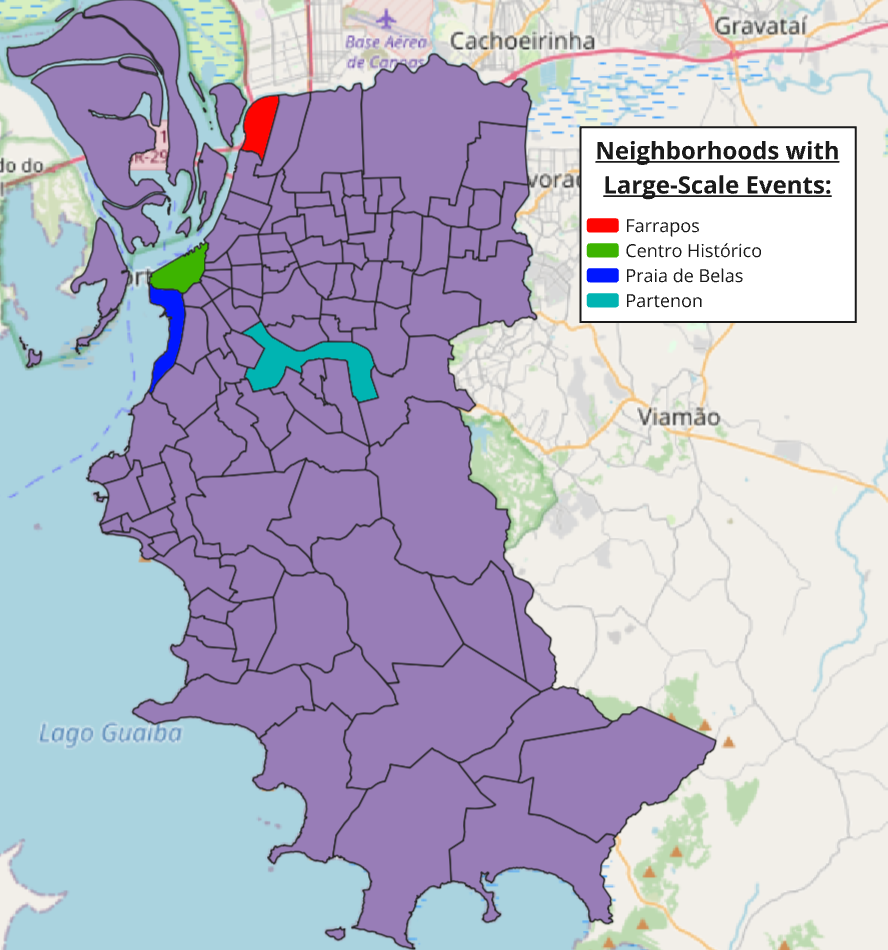
\includegraphics[width=0.6\textwidth]{Figures/CityViewNeighborhoods.png}
  \caption{The 94 neighborhoods of Porto Alegre, Brazil. All 94 neighborhoods of the city are included in all our experiments, with four specific neighborhoods highlighted for their additional routines, utilized in our large-scale experiments (Section~\ref{sec:large_scale}).} 
  \label{fig4:city_view}
\end{figure}

We utilized the OpenStreetMap database~\footnote{OpenStreetMaps is available at: \url{https://www.openstreetmap.org/}} to extract the geographic coordinates (latitude and longitude) of buildings and amenities within Porto Alegre that could serve as points of interest for the population, such as schools and pharmacies.
These points of interest were distributed across the city's neighborhoods. Each region in the model includes the following $P$s: \textit{home}, \textit{work}, \textit{school}, \textit{marketplace}, \textit{pharmacy}, and \textit{gas\_station}. Additionally, some regions may feature other $P$s, such as \textit{shopping\_malls}, \textit{hospitals}, \textit{universities} or \textit{stadiums}.
The modeled environment comprises 94 $R$s and a total of 504 $P$s. For the experiments described in this paper, each region contains at most one $P$ of each type, such as one \textit{home} and one \textit{pharmacy} per neighborhood. This setup was dictated by the available data, which provided information on population distribution at the neighborhood level but did not specify finer-grained details within neighborhoods. However, this is not a limitation of the proposed model. When more granular data is available, simulation designers can enhance the environment by adding multiple home $P$s within a single region and allocating neighborhood populations accordingly. Appendix~\ref{app:input_environment} provides an example of the syntax needed to inform data for modeling an environment in our simulations.

To model the population in our simulations, we collect data from governmental sources, including the most recent completed census at the time of this publication\footnote{Census Conducted by the Brazilian Institute of Geography and Statistics (IBGE). The data is available at:  \url{https://cidades.ibge.gov.br/brasil/rs/porto-alegre/panorama}}. Census data provided citywide information on the total population, the number of economically active individuals (i.e., workers), the number of students, and the age distribution of the population. However, this information lacked specificity at the neighborhood level.
To address this, additional data was gathered from city administration surveys, which included neighborhood-level details on total population and age distribution~\footnote{Surveys conducted by the Observatory of the City of Porto Alegre (ObservaPOA). Data is available at: \url{http://www.observapoa.com.br/}}\footnote{Surveys conducted by the Empresa Pública de Tecnologia da Informação e Comunicação da Prefeitura de Porto Alegre (PROCEMPA). Data is available at: \url{https://portoalegreemanalise.procempa.com.br/}}.
This information was used to define sampled characteristics for the population, with the following identifiers and categories:
\begin{itemize}
    \item $Age$: Child, Young, Adult, and Elder;
    \item $Occupation$: Student, Worker, and Other.
\end{itemize}

Porto Alegre's total population is $1,409,351$. Since \textit{occupation} data was only available at the city level, all neighborhoods were assigned the same distribution: \textit{students} comprise approximately $21.575\%$ of the population, \textit{workers} $54.706\%$, and \textit{other} $23.718\%$.
The \textit{age} distribution was mapped using the age pyramid, with each category representing a specific range: \textit{child} (0–14 years), \textit{young} (15–24 years), \textit{adult} (25–59 years), and \textit{elder} (60+ years). Each neighborhood has its own unique \textit{age} distribution, while the overall population consists of approximately $18.724\%$ \textit{children}, $15.706\%$ \textit{young}, $50.507\%$ \textit{adults}, and $15.061\%$ \textit{elders}. 

For each neighborhood, a blob was initialized at the corresponding \textit{home} $P$, with its total population determined based on the available neighborhood data and its sampled characteristics determined according to the previously described \textit{age} and \textit{occupation} distributions.
Each blob was also assigned a traceable characteristic, \textit{region of origin}, which indicates where the population resides and begins within the simulation. This traceable characteristic enables the identification of a blob's origin throughout the simulation and ensures that the population returns to their respective residences after completing daily activities. Moreover, blobs originating from different regions cannot be merged, as their traceable characteristics remain distinct, preserving information about their place of origin.
Appendix~\ref{app:input_population} provides an example of the input data necessary for modeling an initial population in our simulations.
For all experiments, a \textit{cycle} was defined as 24 \textit{cycle steps}, representing a full day and its hours, respectively. The following sections present results obtained from various simulation scenarios, illustrating the model's capacity to capture population dynamics effectively.


\subsection{Case Study 1: Random Walk}
\label{sec:random_walk}

Gonzalez et al.~\citep{gonzalez2008understanding} provide valuable insights into the dynamics of urban populations, which serve as a foundation for our abstracted urban mobility model. They highlight two significant observations: first, individuals tend to visit a select few locations repeatedly, and second, there is a certain level of randomness in their daily movements, akin to a Lévy flight random walk.
A Lévy flight is a random walk pattern characterized by jumps of varying lengths, following a Lévy heavy-tailed probability distribution. In practical terms, this means that the Lévy flight predominantly consists of short jumps, with fewer long jumps.

To simulate this behavior, we have implemented a Lévy plugin, which introduces a new action type called the \textit{levy walk}. Appendix~\ref{app:plugin} presents an example of how new action types can be incorporated into our simulations using plugins. This action involves sampling distances from a Lévy distribution and moving a certain portion of the population from a certain origin $P_i$ to a destination $P_j$ corresponding to the sampled distance.
For each $P$, we calculate a histogram of distances to other $P$s, grouping them into bins based on a specified distance grouping value. Figure~\ref{fig5:node_distances} illustrates the histogram of distances between $P$s, with each bin representing a range of 500 meters.

\begin{figure}[ht]
 \centering
  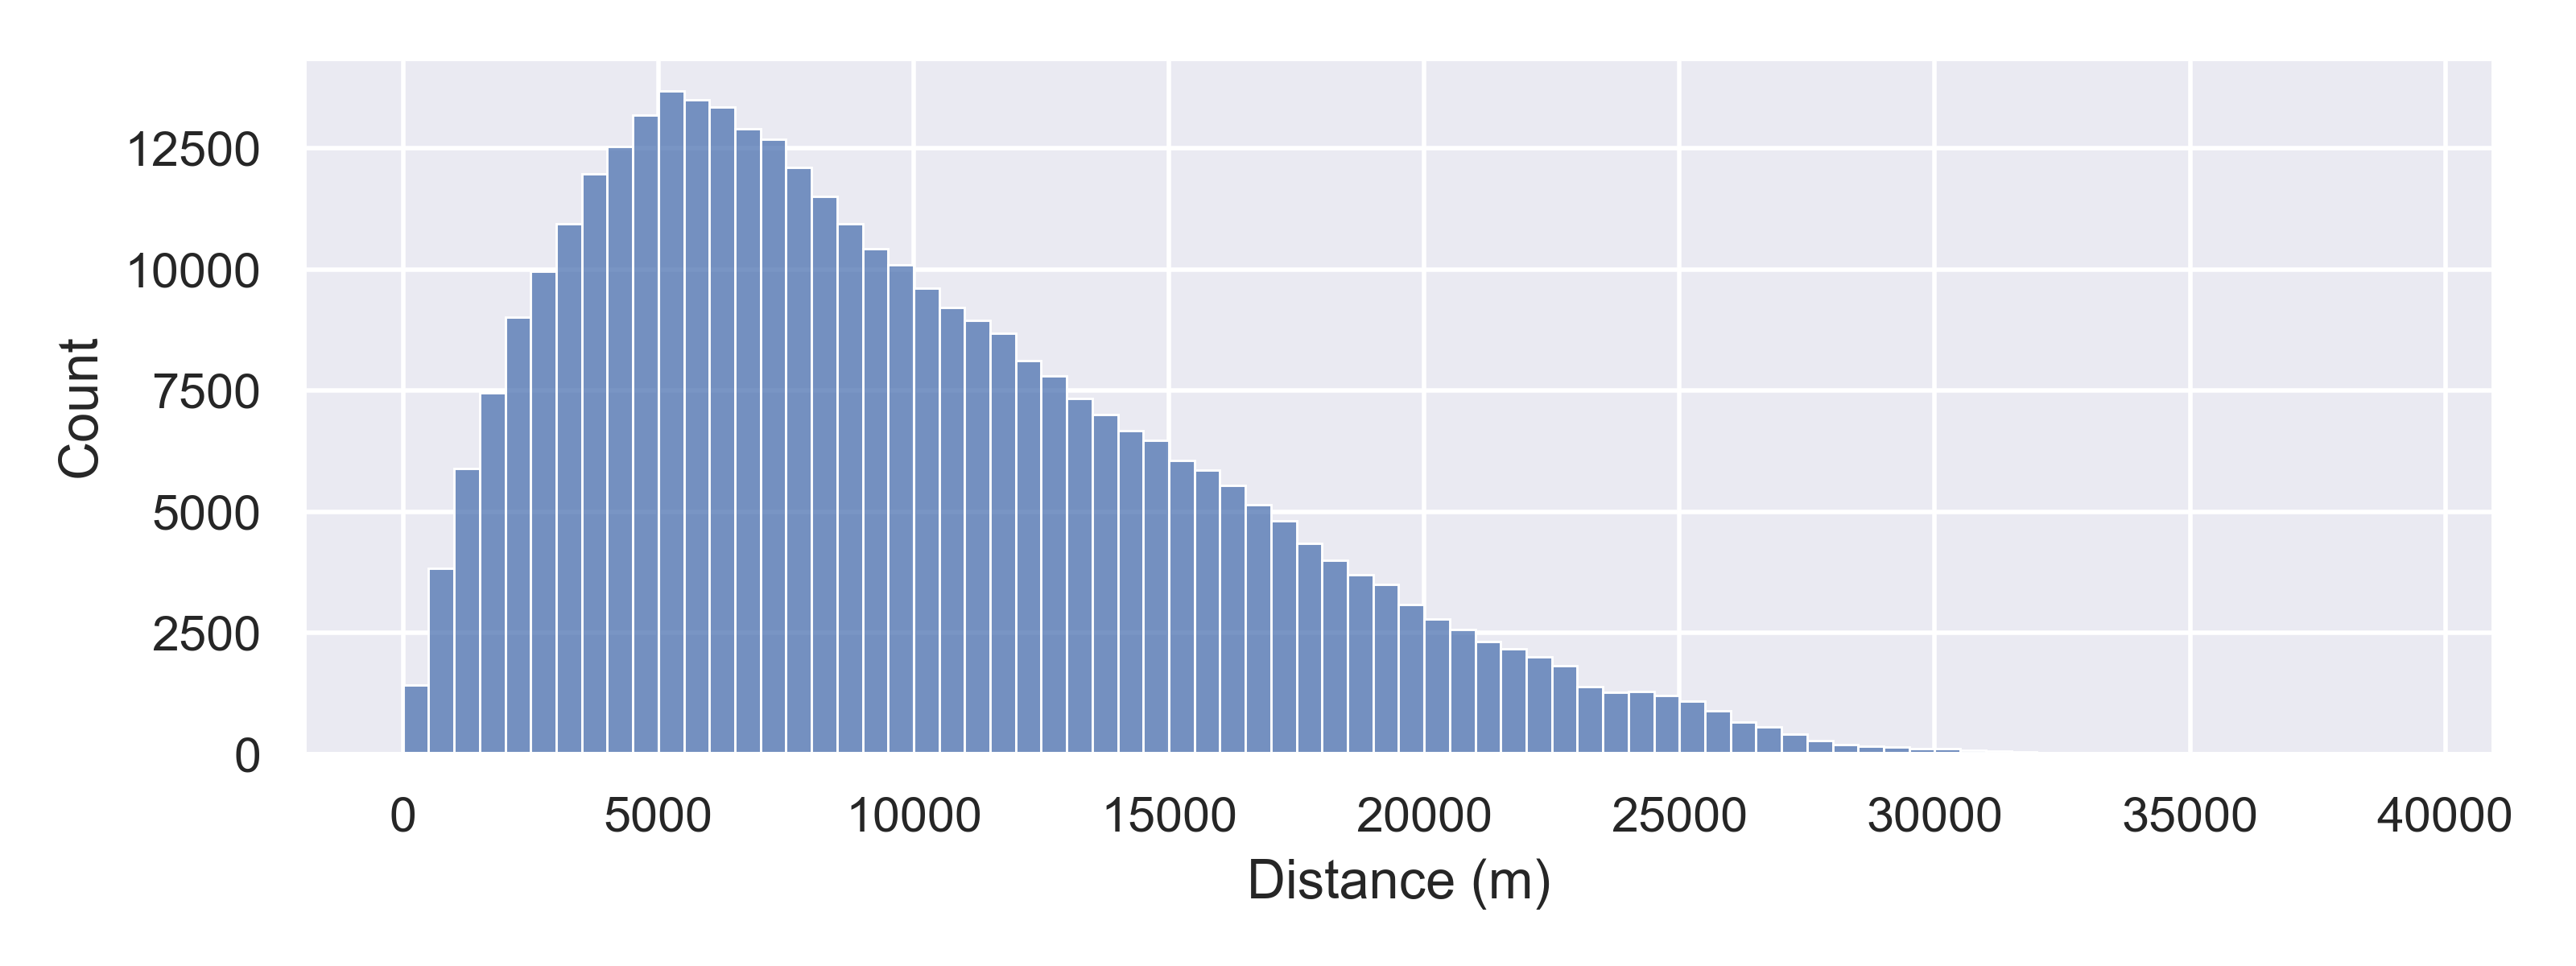
\includegraphics[width=0.95\textwidth]{Figures/NodeDistances.png}
  \caption{ Histogram of distances between points of interest ($P$s). Each bin represents a range of 500 meters.} 
  \label{fig5:node_distances}
\end{figure}

When the \textit{levy walk} action is triggered, the population at the origin $P_i$ is uniformly divided into packets to be moved. Upon sampling a distance, the \textit{levy walk} action randomly assigns a population packet to one of the $P$s within that distance group. Since the Lévy distribution is heavy-tailed (see Figure~\ref{fig6:levy_distributions}), it is possible to sample a distance that exceeds the farthest $P$, even if it is not very probable. In such cases, another distance is sampled from the distribution. Similarly, if there are no available $P$s within the sampled distance group, a new distance will be sampled.

A \textit{levy walk} action $A_i$ incorporates additional parameters $\bm{V}_{i}$ (Section~\ref{sec:routines}) to enhance its functionality. These parameters include the scale parameter ($levy\_scale$), which governs the Lévy distribution; the movement probability parameter ($levy\_prob$), which determines the likelihood of a population packet being moved; the packet size parameter ($levy\_pkt$), representing the group size that undergoes the random walk; and an optional label parameter ($levy\_label$), enabling the selection of specific types of $P$s as potential destinations. 
Additionally, a \textit{levy walk} action $A_i$ requires a population template $T_{i}$ to specify the desired population profile being affected.
These parameters enable the simulation of random walk behavior across multiple scales: spatial scales, by adjusting the $levy\_scale$ parameter to match the simulated environment, and population scales, by modifying $levy\_pkt$, which allows for the movement of large populations or individual entities (i.e., a blob with a total population of 1).

In our experiments, we design a global routine ($GRo$) that utilizes \textit{levy walk} actions to disperse the working and student populations across the city throughout the day. Actions targeting workers relocate the population from a ``home" $P_h$ to a ``work" $P_w$, utilizing a population template with criteria such as $Occupation = Worker$ and $Age = [Young, Adult, Elder]$. These actions occur at each cycle step, with a higher movement probability ($levy\_prob$) during the morning and afternoon (specifically, steps 7 through 18).
Actions targeting students relocate the population from a ``home" $P_h$ to a ``school" $P_s$, using a population template with criteria such as $Occupation = Student$ and $Age = [Child, Young, Adult]$. These actions are executed only at specific cycle steps. Furthermore, the simulation routine includes \textit{move population} actions in all ``work" and ``school" $P$s, returning a portion of their current population to their respective ``home" $P$ of each blob they contain. In both cases, the \textit{region of origin} traceable characteristic of each blob allows us to identify the ``home'' $P$s where students and workers originate and return at the end of the day.

Subsequently, we conducted experiments by varying the $levy\_scale$ parameter in all \textit{levy walk} actions to assess the population movements throughout the simulation. We define ``displacement" as the movement of an individual from one $P_i$ to another $P_j$, as part of the levy plugin.
In the case of a blob $B_i$ with a total population $TP_i = 250$, each movement between points of interest accounts for 250 displacements. All simulations maintain a population packet size of $levy\_pkt = 250$, and the $P$s are grouped based on the distance to an origin $P$, with intervals of 500 meters, as depicted in Figure~\ref{fig5:node_distances}.

The experimental results are illustrated in Figure~\ref{fig6:levy_distributions}. All simulations consider a total population of $1,409,351$. The x-axis represents the distance traveled during each displacement, grouped into 500-meter intervals.
The y-axis indicates the total number of displacements that occurred at each levy configuration. The graph demonstrates that different values of the $levy\_scale$ parameter produce distinct distributions, where higher values yield more widely dispersed distributions of displacements, as observed in a simulation where $levy\_scale = 10$.

\begin{figure}[ht]
 \centering
  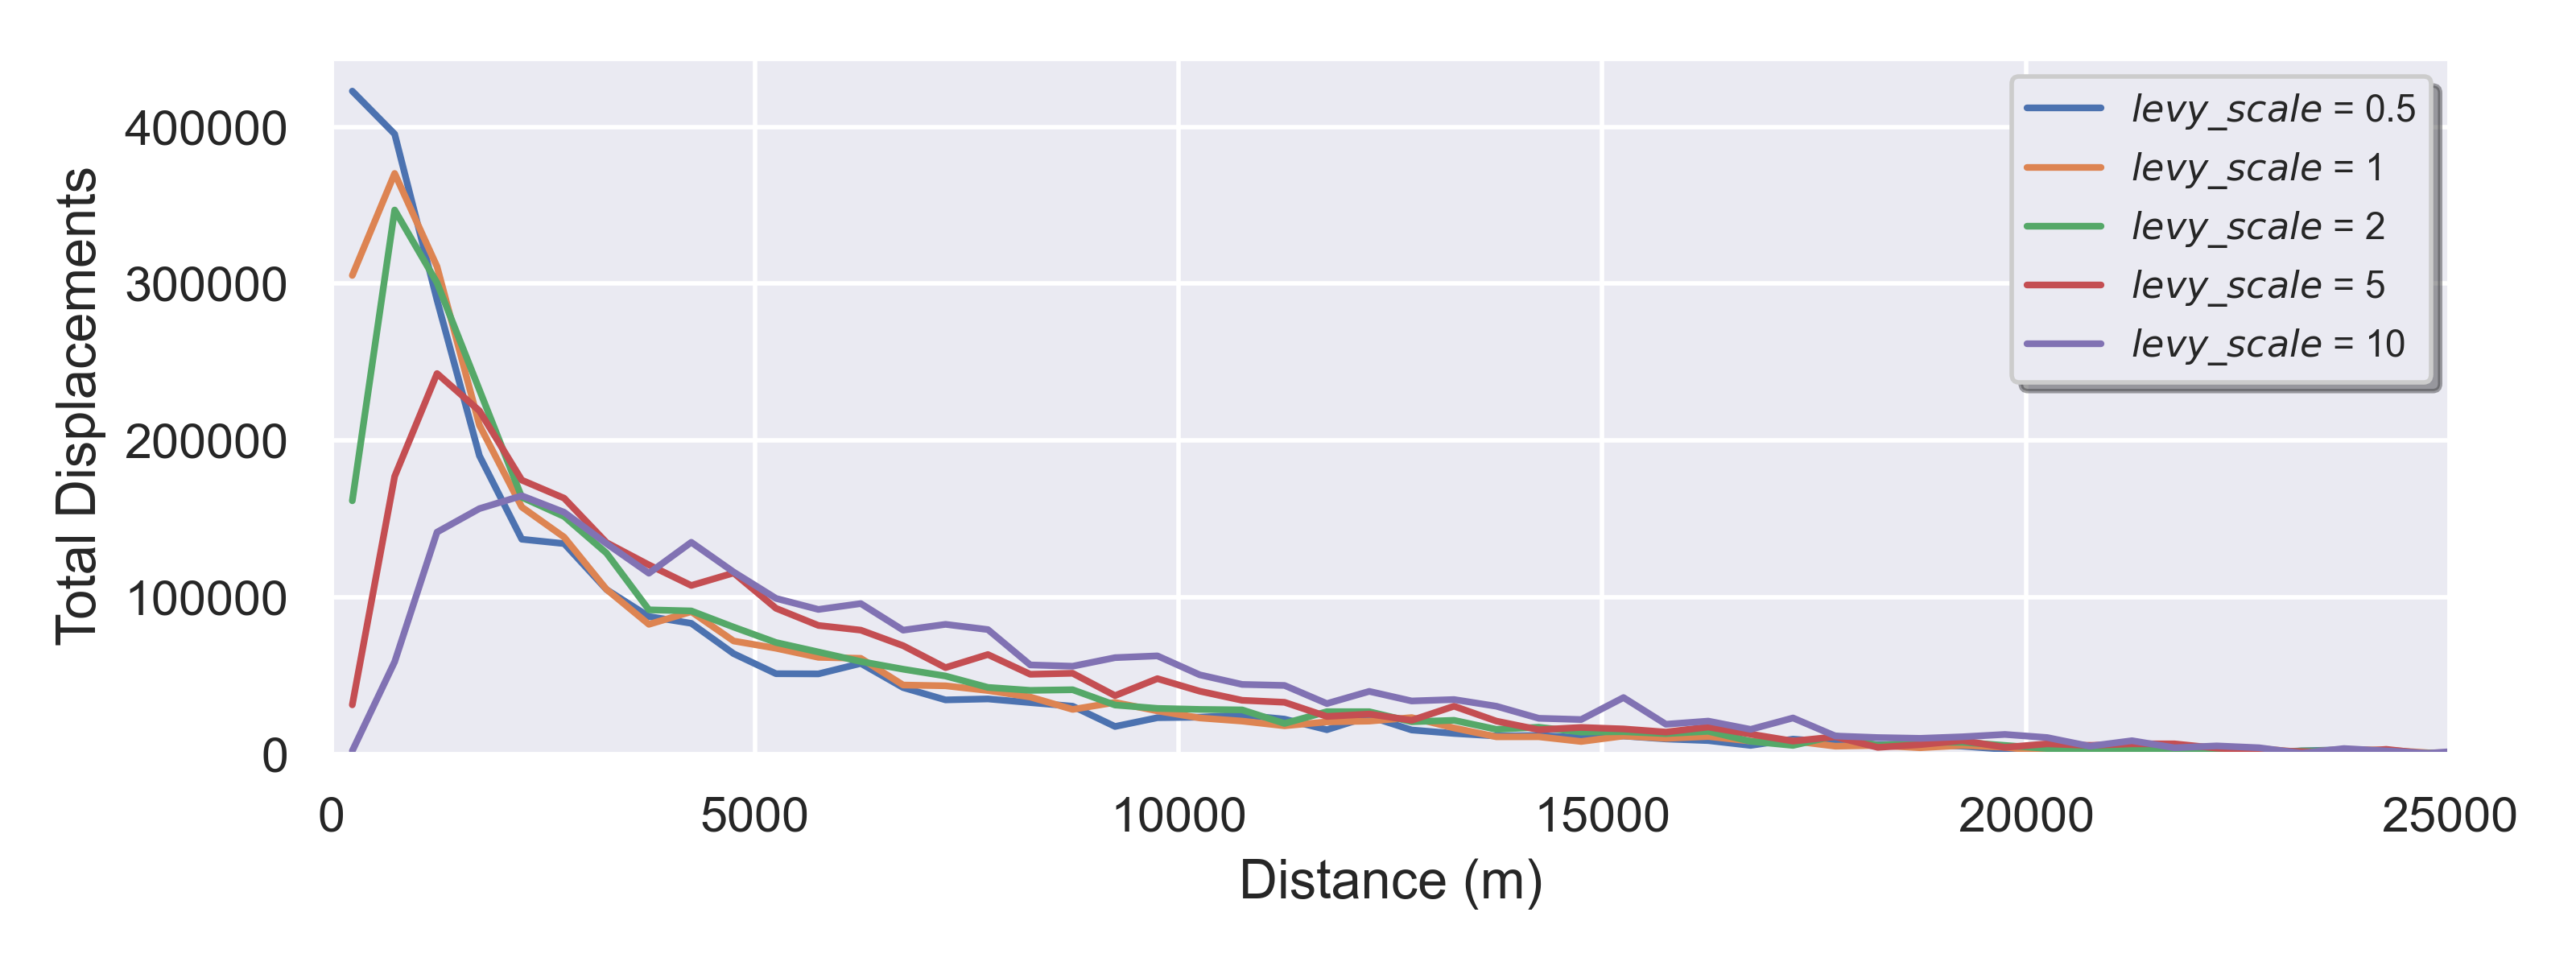
\includegraphics[width=0.95\textwidth]{Figures/Levy_Distributions.png}
  \caption{ Population displacement experiments. The x-axis represents the distance traveled during a displacement and is grouped in ranges of 500 meters. The y-axis represents the total number of displacements that traveled a certain distance. All simulations consider a total population of $1,409,351$; a population packet size of $levy\_pkt = 250$, which represents the group size that undergoes the random walk; and $P$s grouped by distance in ranges of 500 meters, as presented in Figure~\ref{fig5:node_distances}.} 
  \label{fig6:levy_distributions}
\end{figure}
%python .\movement_displacement_comparison.py --p levy_parameter_tests_94 --b 500 --e WorkSchool94-BW_500-S_250  WorkSchool94-BW_500-S_500 WorkSchool94-BW_500-S_1000  WorkSchool94-BW_500-S_2500 WorkSchool94-BW_500-S_5000 --x 25000 --l "Scale = 0.5" "Scale = 1" "Scale = 2" "Scale = 5" "Scale = 10"

For the remaining experiments in this work, we adopt a scale parameter of $levy\_scale = 2$ (represented by the green line in Figure~\ref{fig6:levy_distributions}). This particular value was determined empirically, as approximately $50\%$ of the displacements observed in simulations using this parameter occurred within a 2km radius of the origin $P$. Such displacements align with typical daily movements within a single neighborhood or between neighboring neighborhoods. However, this value can be adjusted to suit different environments, depending on the needs of the simulation designers. 

Furthermore, we introduce an additional parameter, named $Restriction$, for the \textit{levy walk} action to model movement restrictions.
This parameter acts as a factor that reduces the total population being moved by each \textit{levy walk} action, e.g., an $Restriction = 0.25$ would cause a \textit{levy walk} action to move only $\approx75\%$ of the population it would without the restriction. It allows for the simulation of varying population flows on different days of the week (e.g., weekends with different flow patterns than weekdays) or the simulation of population lockdown during a pandemic scenario. Figure~\ref{fig7:movement_restriction} illustrates the results obtained by conducting a baseline experiment (without any restriction) and three other experiments involving different levels of movement restrictions. As previously mentioned, all simulations consider a scale parameter of $levy\_scale = 2$.

\begin{figure}[ht]
 \centering
  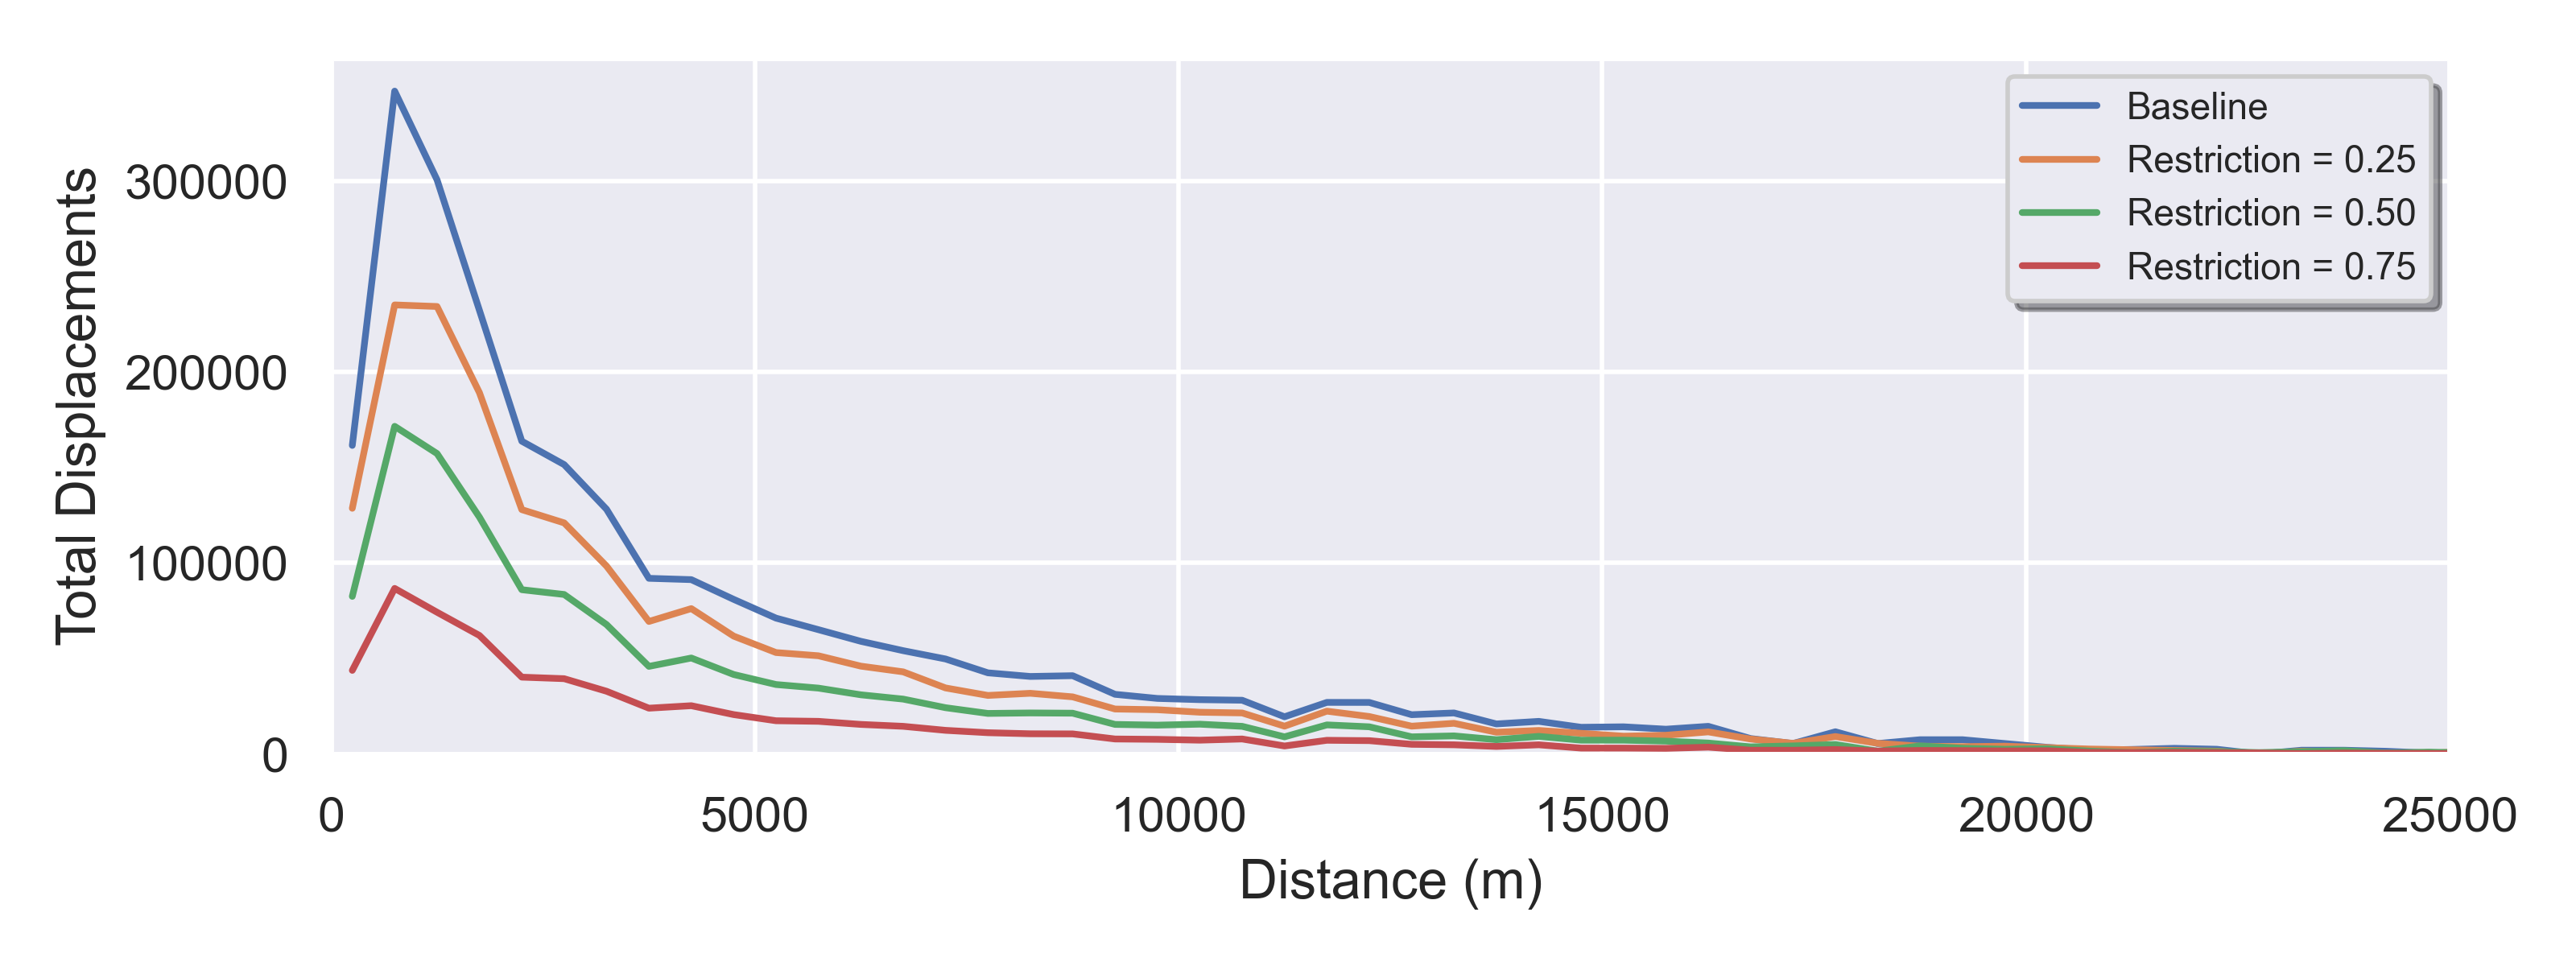
\includegraphics[width=0.98\textwidth]{Figures/MovementRestriction.png}
  \caption{Simulation of Movement Restriction with the \textit{levy walk} action. All simulations consider a scale parameter of $levy\_scale = 2$. The $Restriction$ parameter acts as a factor that reduces the total population being moved by each \textit{levy walk} action.} 
  \label{fig7:movement_restriction}
\end{figure}
%python .\movement_displacement_comparison.py --p isolation_tests --b 500 --e Baseline Baseline-Iso_25 Baseline-Iso_50 Baseline-Iso_75 Baseline-Iso_100 --l Baseline "Restriction = 0.25" "Restriction = 0.50" "Restriction = 0.75" "Restriction = 1.00" --x 25000


\subsection{Case Study 2: Large-Scale Events}
\label{sec:large_scale}

We also investigate the ability to simulate occasional events that disrupt the population's daily routines, such as sports matches or musical concerts that occur on a weekly or monthly basis.
To evaluate the impact of these large-scale events on mobility patterns, we compare their effects against a baseline scenario with no events. Furthermore, we examine how multiple concurrent events compete for the available population, highlighting the dynamics of population distribution.

To simulate these events, we implemented an additional plugin, which introduces a new action type called \textit{gather population}. This action involves gathering the population from nearby $P$s and relocating them to a designated destination $P_d$. 
A \textit{gather population} action $A_j$ considers a $gather\_quantity$ additional parameter (in $\bm{V}_{j}$)  to describe the total population to be relocated towards the destination $P_d$. 
The population quantity to be moved from each nearby $P$ is determined by the population available at the origin $P$ and the distance to the destination.
Once the population quantity that should be moved from each origin $P$ is determined, the \textit{gather population} action is further broken down into multiple \textit{move population} actions. Each of these \textit{move population} actions is responsible for transferring the population from an origin $P$ to the destination $P_d$, ensuring that each origin $P$ contributes to the movement.

For these experiments, we consider the routines of workers and students as a baseline simulation, utilizing a scale parameter of $levy\_scale = 2$ as described in Section~\ref{sec:random_walk}.
Furthermore, we incorporate four large-scale events into the simulation, each occurring at a specific cycle step. These events are characterized by a \textit{gather population} action, which requests the movement of 500,000 individuals to a designated destination $P$. The details of the events are specified as follows, considering the regions illustrated in Figure~\ref{fig4:city_view}: 

\begin{itemize}
    \item Event $(A)$: A sports event taking place at the Farrapos region stadium;
    \item Event $(B)$: A sports event happening at the Praia de Belas region stadium;
    \item Event $(C)$: A commercial event held at the marketplace in the Centro Histórico region; and
    \item Event $(D)$: A cultural event occurring at our University in the Partenon region.
\end{itemize}

All events are scheduled to occur at cycle step 19, i.e., at 7:00 PM. Given that the city's total population is 1,409,351, and the events require a total of 2,000,000 individuals, the events will compete for the available population if they all occur simultaneously in a single simulation.
In addition, we model a scenario where some large-scale events take place at different cycle steps. In this alternate scenario, event C occurs at cycle step 9 (i.e., 9:00 AM), while event D occurs at cycle step 14 (i.e., 2:00 PM).

Table~\ref{tbl:results_displacement} provides an overview of the simulation results, including the total population displacements, the average displacement per city inhabitant, and the proportion of total displacements compared to the baseline simulation. Baseline means the ``normal life'' of the city, and the different scenarios in the table indicate the population displacements as a function of the existence of the events. For instance, the ``Baseline+AB'' scenario considers the Baseline in addition to Event A and Event B. In the two last lines of Table~\ref{tbl:results_displacement}, we show the results of the Baseline with the existence of the four large-scale events occurring at the same time and with some occurring at different cycle steps.


\begin{table}[ht]
\footnotesize
\centering
\caption{Results of the large-scale event simulations. Data includes the total population displacements, the average displacement per inhabitant of the city, and a proportion of total displacements compared to the baseline simulation. The ``Baseline+AB'' scenario, for example, considers the Baseline in addition to Event A and Event B.}
\label{tbl:results_displacement}
\begin{tabular}{@{}lccc@{}}
\toprule
Experiment Name        & \begin{tabular}[c]{@{}c@{}}Total\\ Displacements\end{tabular} & \begin{tabular}[c]{@{}c@{}}Average Displacements\\ per inhabitant\end{tabular} & \begin{tabular}[c]{@{}c@{}}Increase over\\ Baseline\end{tabular}  \\ \midrule
Baseline               & 2,570,658                                                                                                                                                 & 1.8240                                                                                                                                                 & ---             \\ \midrule
Baseline+A             & 3,290,469                                                                                                                                                 & 2.3347                                                                                                                                                 & 28.00\% \\ %1.2800           \\
Baseline+B             & 3,300,782                                                                                                                                                 & 2.3421                                                                                                                                                 & 28.40\% \\ %1.2840           \\
Baseline+C             & 3,289,002                                                                                                                                                 & 2.3337                                                                                                                                                 & 27.94\% \\ %1.2794           \\
Baseline+D             & 3,281,102                                                                                                                                                 & 2.3281                                                                                                                                                 & 27.64\% \\ \midrule %1.2764           \\ \midrule
Baseline+AB            & 3,786,856                                                                                                                                                 & 2.6870                                                                                                                                                 & 47.31\% \\ %1.4731           \\
Baseline+AC            & 3,748,417                                                                                                                                                 & 2.6597                                                                                                                                                 & 45.82\% \\ %1.4582           \\
Baseline+AD            & 3,804,017                                                                                                                                                 & 2.6991                                                                                                                                                 & 47.98\% \\ %1.4798           \\
Baseline+BC            & 3,738,497                                                                                                                                                 & 2.6526                                                                                                                                                 & 45.43\% \\ %1.4543           \\
Baseline+BD            & 3,839,126                                                                                                                                                 & 2.7240                                                                                                                                                 & 49.34\% \\ %1.4934           \\
Baseline+CD            & 3,826,094                                                                                                                                                 & 2.7148                                                                                                                                                 & 48.84\% \\ \midrule %1.4884           \\ \midrule
Baseline+ABC           & 4,042,413                                                                                                                                                 & 2.8683                                                                                                                                                 & 57.25\% \\ %1.5725           \\
Baseline+ABD           & 4,109,929                                                                                                                                                 & 2.9162                                                                                                                                                 & 59.88\% \\ %1.5988           \\
Baseline+ACD           & 4,069,223                                                                                                                                                 & 2.8873                                                                                                                                                 & 58.29\% \\ %1.5829           \\
Baseline+BCD           & 4,081,563                                                                                                                                                 & 2.8961                                                                                                                                                 & 58.78\% \\ \midrule %1.5878           \\\midrule
Baseline+ABCD          & 4,235,926                                                                                                                                                 & 3.0056                                                                                                                                                 & 64.78\% \\ %1.6478           \\ 
Baseline+ABCD+DiffStep & 4,638,329                                                                                                                                                 & 3.2911                                                                                                                                                 & 80.43\% \\ \bottomrule %1.8043           \\ \bottomrule
\end{tabular}
\end{table}



Figure~\ref{fig8:results_displacements} presents the results of the simulation of large-scale events.
Figure~\ref{fig8a:results_displacement_single} visualizes the results of five simulations: the Baseline simulation (no events), a simulation with only Event A, a simulation with only Event B, only Event C, and only Event D. 
As indicated by the data in Table~\ref{tbl:results_displacement}, simulations where only a single large-scale event occurs yield a similar number of total displacements. However, the different locations where each event occurred (i.e., different destination $P$s) and the available population nearby cause each simulation to have other total displacement counts for different distances. For example, the ``Baseline+A'' simulation (shown in orange in Figure~\ref{fig8a:results_displacement_single}) presents an increased total displacement count near the $20,000m$ distance.

\begin{figure}[!htbp]
  \centering
  \subfloat[Experiments include the Baseline scenario (no events), a scenario with only Event A, only Event B, only Event C, and only Event D.]
  {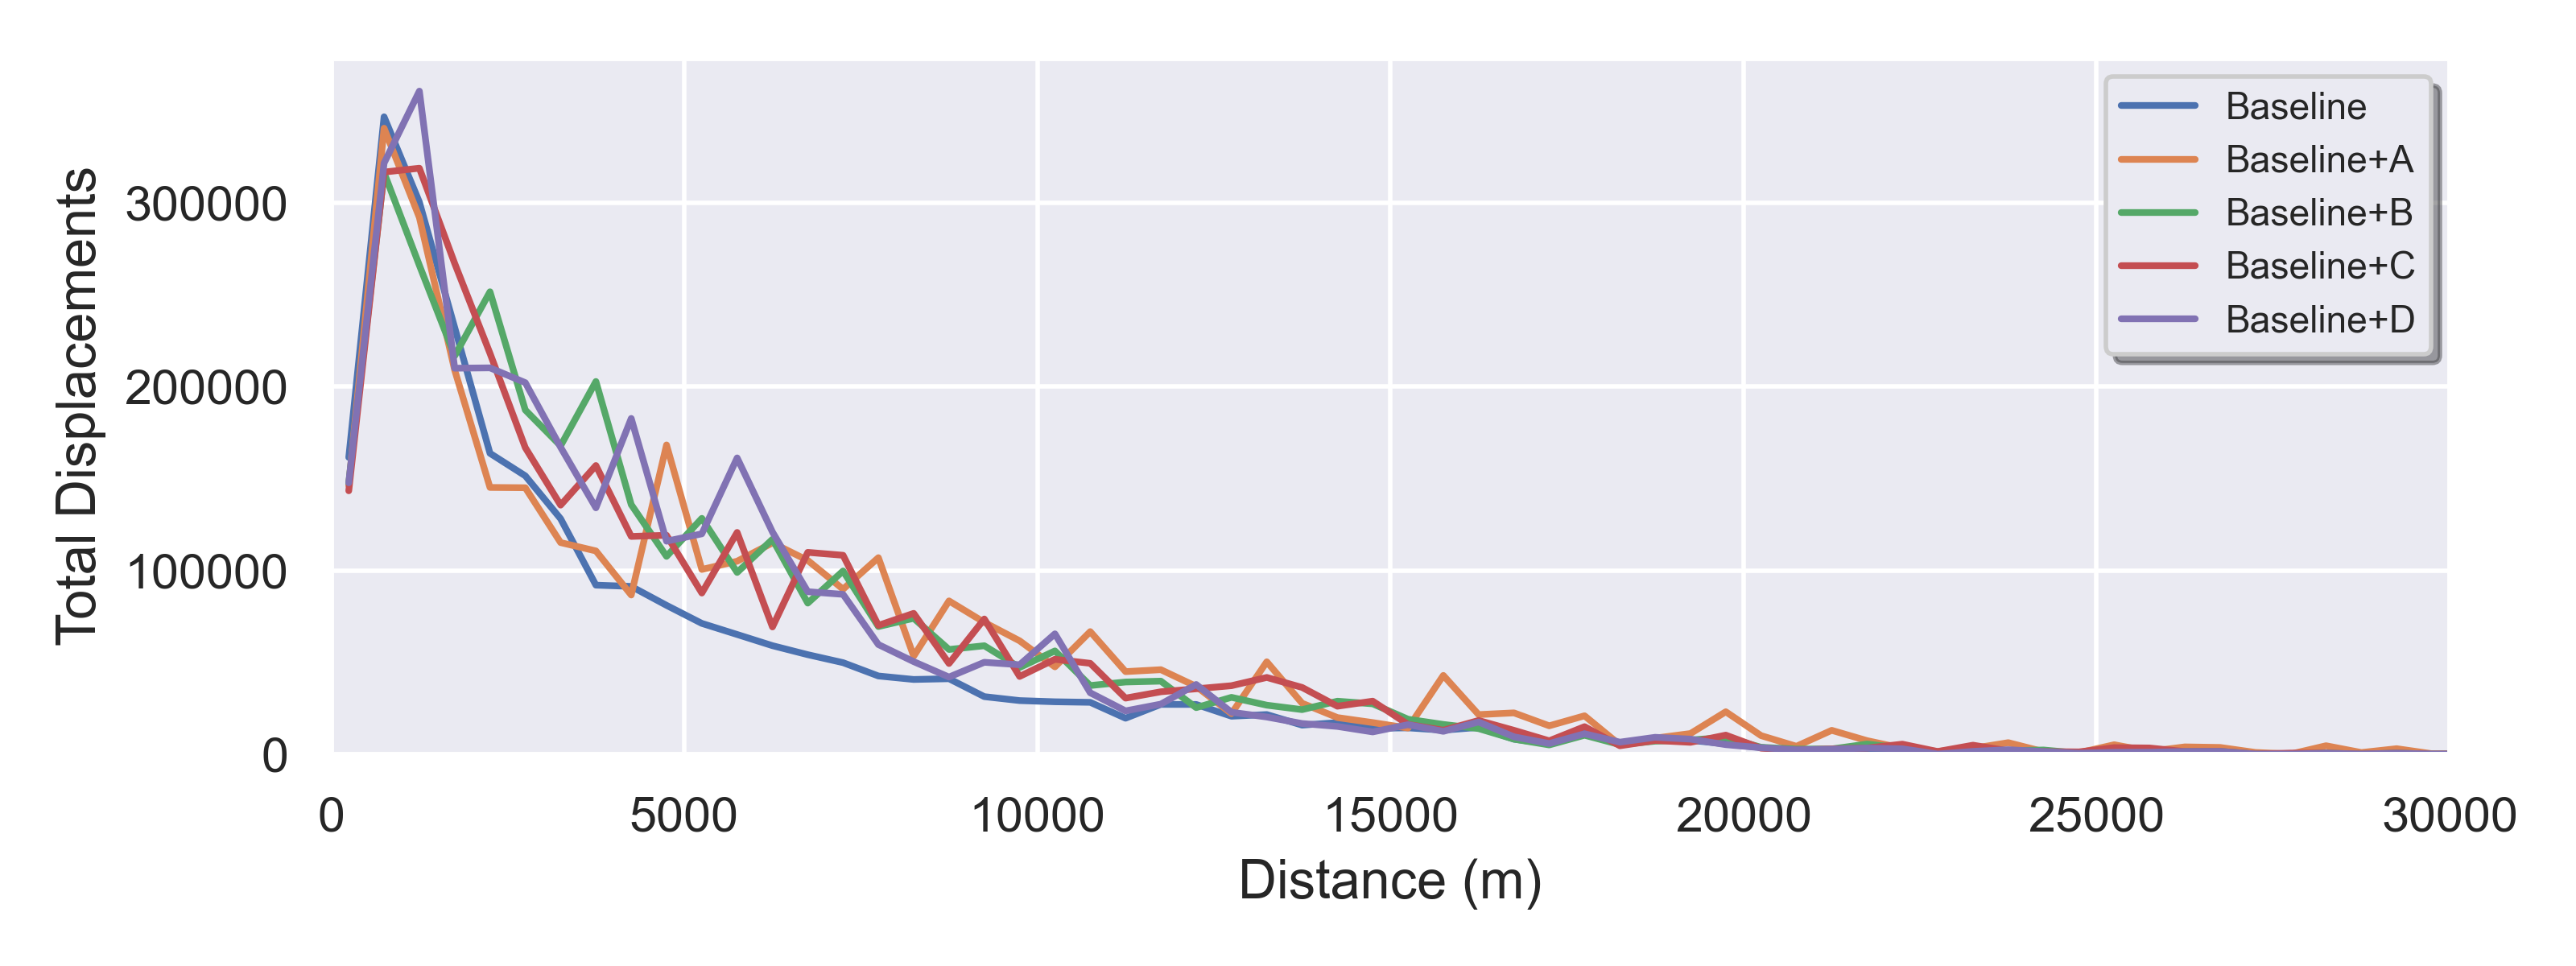
\includegraphics[width=0.95\textwidth]{Figures/Displacement_SingleEvent.png}
  \label{fig8a:results_displacement_single}}\\
  %python .\movement_displacement_comparison.py --p large_scale_event --b 500 --e Baseline Baseline+A_Dist Baseline+B_Dist Baseline+C_Dist Baseline+P_Dist --l Baseline Baseline+A Baseline+B Baseline+C Baseline+D --x 30000
  \subfloat[Experiments include the Baseline scenario and four other scenarios with three events occurring at the same cycle step (i.e., only one event missing in each).]
  {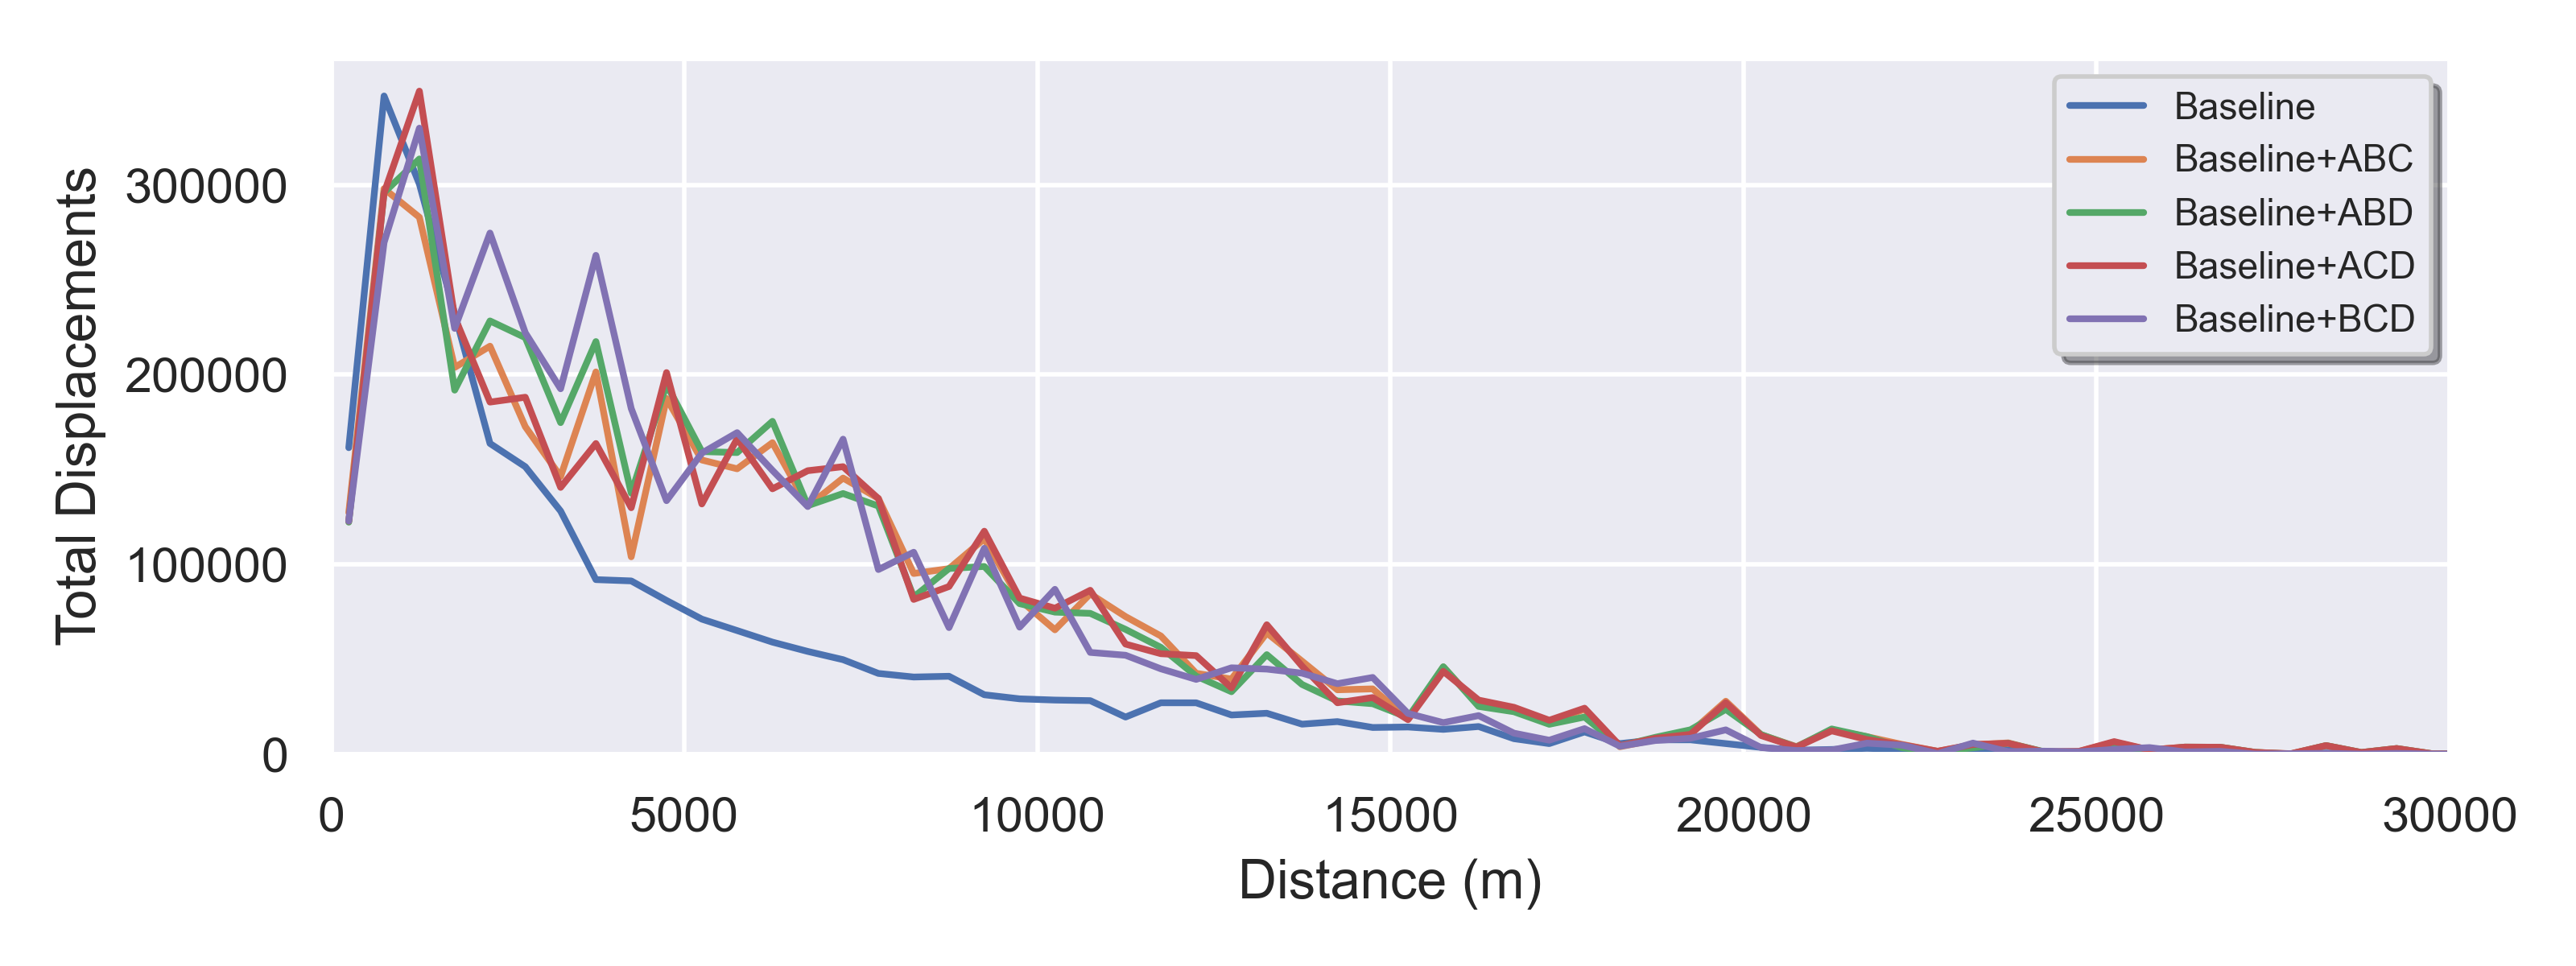
\includegraphics[width=0.95\textwidth]{Figures/Displacement_ThreeEvents.png}
  %python .\movement_displacement_comparison.py --p large_scale_event --b 500 --e Baseline Baseline+ABC_Dist Baseline+ABP_Dist Baseline+ACP_Dist Baseline+BCP_Dist --l Baseline Baseline+ABC Baseline+ABD Baseline+ACD Baseline+BCD --x 30000
  \label{fig8b:results_displacement_three}}\\
  \subfloat[Experiments include the Baseline scenario, the Baseline in addition to all four events occurring at the same cycle step, and the Baseline in addition to all four events with some occurring at different cycle steps (DiffStep).]
  {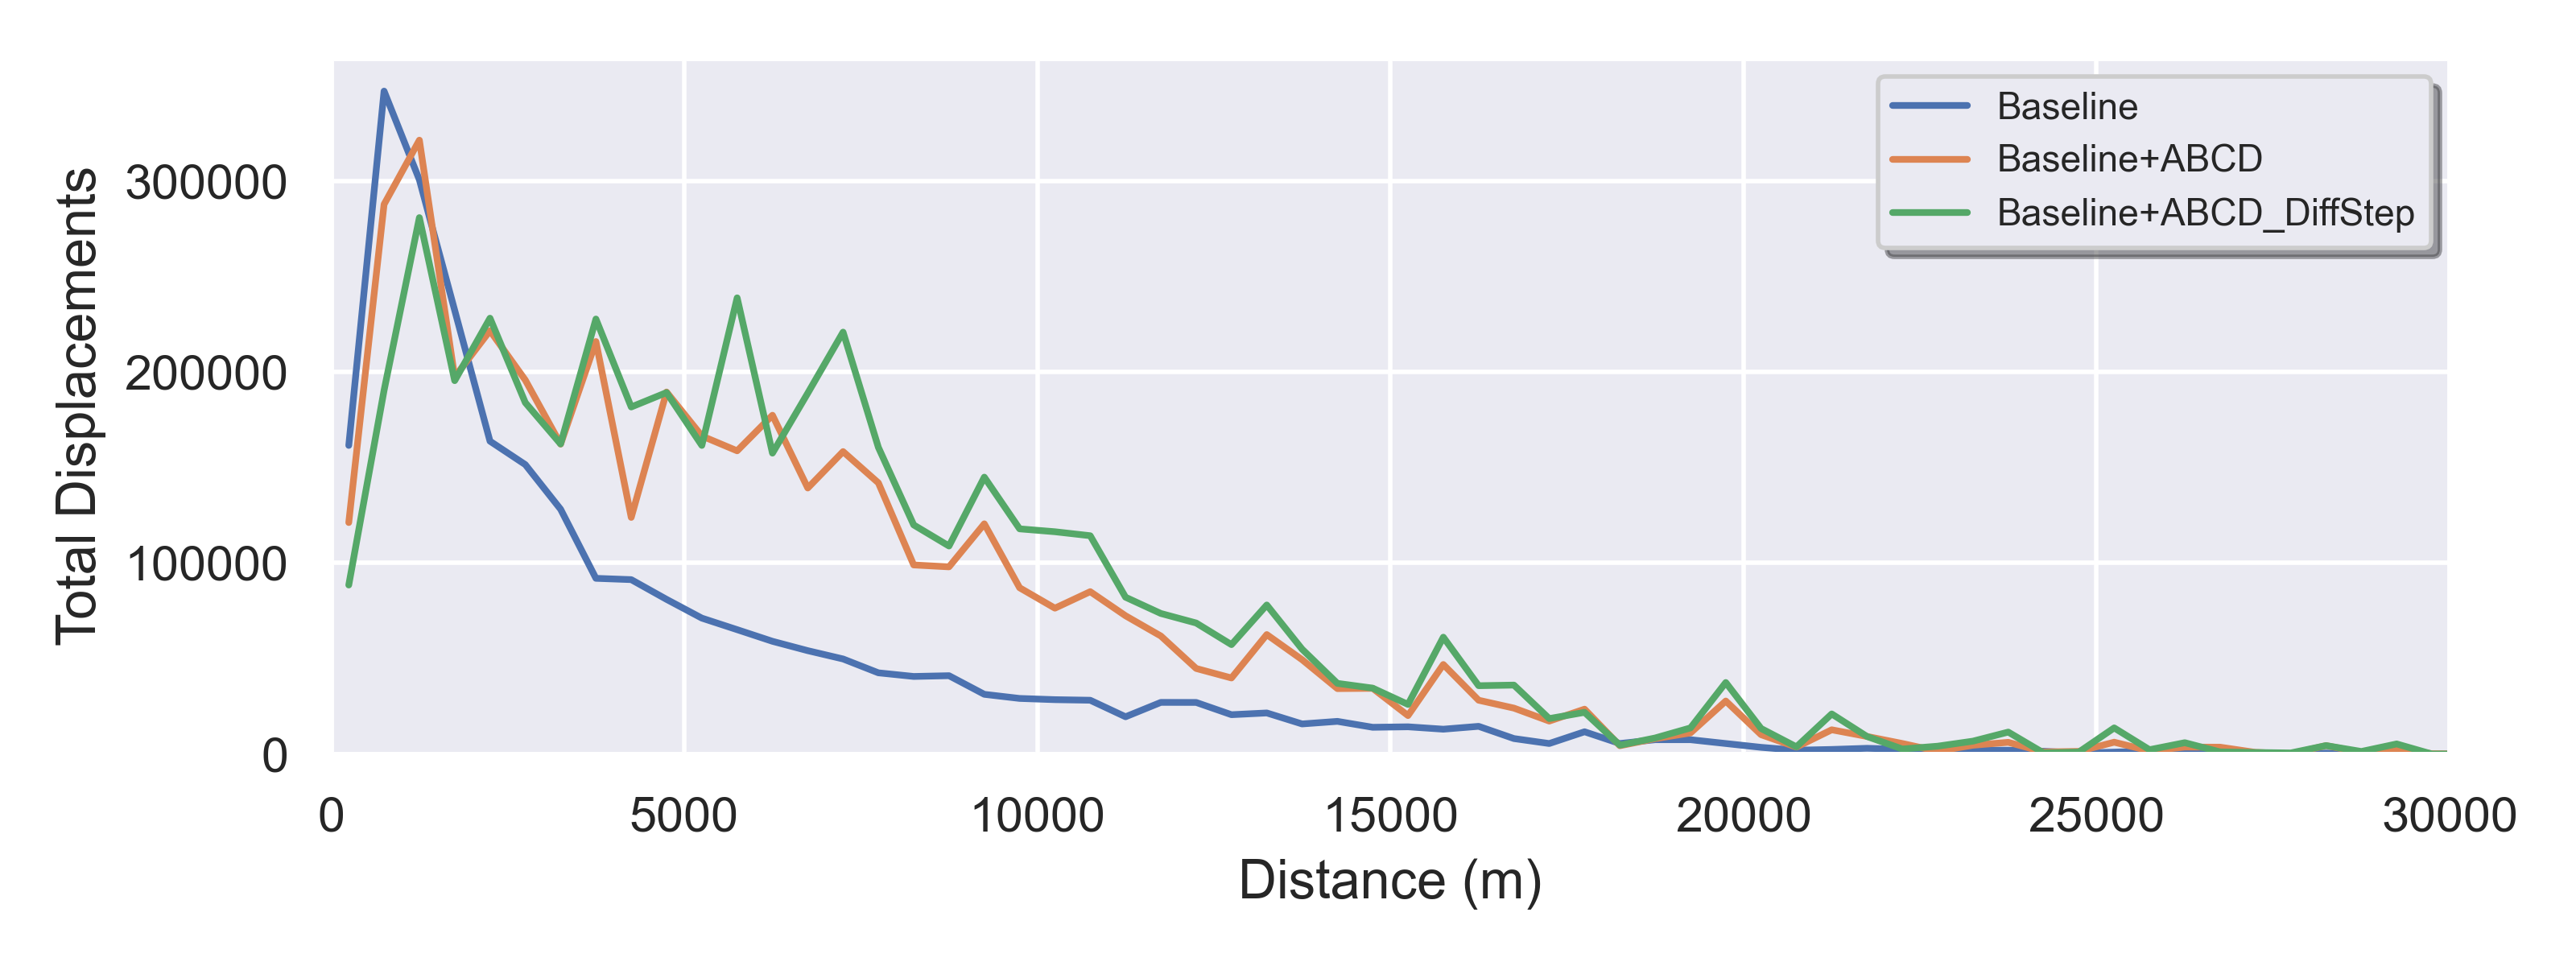
\includegraphics[width=0.95\textwidth]{Figures/Displacement_AllEvents.png}
  \label{fig8c:results_displacement_all}}
  %python .\movement_displacement_comparison.py --p large_scale_event --b 500 --e Baseline Baseline+ABCP_Dist Baseline+DiffStep_ABCP_Dist --l Baseline Baseline+ABCD Baseline+ABCD_DiffStep --x 30000
  \caption{Simulation of large-scale events.}
 \label{fig8:results_displacements}
\end{figure}

Figure~\ref{fig8b:results_displacement_three} illustrates the results of five simulations, starting with the baseline simulation and followed by simulations with three events occurring at the same cycle step (i.e., only one event missing in each). 
As expected, and as indicated by the data in Table~\ref{tbl:results_displacement}, the inclusion of additional events led to an increase in total displacements compared to the baseline simulation. However, it is important to note that although each event requests the movement of 500,000 individuals, the total displacements of three events do not increase by 1,500,000 compared to the baseline simulation. This is because individuals can move directly from their respective origin $P$s (such as work or school) to the event $P$s. Thus, workers can travel from their ``work" $P$s to the event directly, and students can travel from their ``school" $P$s to the event without the need to return to their ``homes" before going to the events. Moreover, Events A, B, and C separately contribute to $\approx730,000$ additional displacements to the baseline simulation, as shown in ``Baseline+A", ``Baseline+B", and ``Baseline+C" in Table~\ref{tbl:results_displacement}, respectively.
In simulations where the three events occur simultaneously (i.e., ``Baseline+ABC''), the events will compete for the available population in nearby neighborhoods, resulting in a reduced total population attending each event. Such result is presented in the last column of Table~\ref{tbl:results_displacement}, where the number of displacements increased over the baseline is $57.25\%$ for simulation ``Baseline+ABC''. This is a lower amount than the sum of increased displacements of simulations ``Baseline+A", ``Baseline+B", and ``Baseline+C", which were $28.00\%$, $28.40\%$, and $27.94\%$, respectively.

Figure~\ref{fig8c:results_displacement_all} presents the results of three simulations: the baseline simulation, a simulation with all four events occurring simultaneously, and a simulation with some events taking place at different cycle steps. As demonstrated by the data in Table~\ref{tbl:results_displacement}, the simulation where events occurred at different cycle steps exhibited a significantly higher number of displacements than the simulation with all four events happening simultaneously. This increase in the number of displacements
can be attributed to two factors. Firstly, there is reduced competition for the available population when events are staggered. Secondly, individuals have the opportunity to attend multiple events throughout the day, increasing their individual displacements.

\subsection{Case Study 3: Epidemic Contagion and Vaccination}
\label{sec:contagion}

Next, we explore our model's ability to simulate behaviors observed over extended temporal scales, focusing on their long-term effects on the population. Specifically, we model the spread of an infectious disease as the population moves throughout the city, analyzing its progression over multiple simulation cycles, which represent consecutive days. Additionally, we evaluate the impact of public policies, such as vaccination campaigns and population lockdowns, on mitigating the disease's spread.

To achieve this, we have implemented an additional plugin that introduces an \textit{infection} action type. This action is based on the SIR model~\citep{kermack1927contribution}, which classifies individuals into one of three states: Susceptible, Infected, or Removed. The ``Removed" state includes individuals who can no longer contribute to further contagion, either due to acquiring immunity (recovered) or death. The numerical dynamics of the SIR model are defined by Equations~\ref{eq:deltaS}, \ref{eq:deltaI}, and \ref{eq:deltaR}.

\begin{equation}
\label{eq:deltaS}
   { \frac{dS}{dt} } =- { \frac{\beta I S}{N} },
\end{equation}

\begin{equation}
\label{eq:deltaI}
   { \frac{dI}{dt} } = { \frac{\beta I S}{N} } - {\gamma I},
\end{equation}

\begin{equation}
\label{eq:deltaR}
   { \frac{dR}{dt} } = {\gamma I},
\end{equation}
where, $\frac{dS}{dt}$, $\frac{dI}{dt}$ and $\frac{dR}{dt}$ represent the rate of change over time for the susceptible, infected, and recovered populations, respectively, in a total population of $N$ individuals. The parameters $\beta$ and $\gamma$ represent the infection and removal rates, respectively. The basic reproduction ratio, denoted as $R_0$, is defined as $R_0 = {\frac{\beta}{\gamma}}$. It is important to note that the total population $N$ remains constant in the SIR model, maintaining equality throughout the simulation.

To monitor the progression of the infection within the population, we introduced a traceable characteristic called \textit{SIR Status} for all blobs in the simulations. This characteristic can take one of three possible values: ``Susceptible", ``Infected", or ``Removed". As outlined in Section~\ref{sec:population}, each blob in the simulation consists of individuals who share the same \textit{SIR Status} value. However, blobs with different \textit{SIR Status} values can coexist within the same $P$, allowing for the simultaneous representation of susceptible, infected, and removed individuals at a given location.

In the context of epidemic simulations, we utilize the routines of workers and students as the baseline, employing a scale parameter of $levy\_scale = 2$ as described in Section~\ref{sec:random_walk}. Additionally, we incorporate the \textit{infection} action into the global routine $GRo$, which occurs at every cycle step. When triggered, the \textit{infection} action identifies the current population with each SIR status in a given $P$ and applies Equations~\ref{eq:deltaS}, \ref{eq:deltaI}, and \ref{eq:deltaR} based on the $\beta$ and $\gamma$ parameters. We conducted experiments considering different values for the basic reproduction ratio ($R_0$), as this value can vary across different countries and cities. We specifically selected $R_0$ values of 2.6, 3.07, and 6.0 based on research conducted on Brazil's COVID-19 data~\citep{dutra2020covidR0, deSouza2020covirR0, dutra2021covidR0}\footnote{Additional research on $R_0$ on Brazilian state capitals available \href{https://www.blogs.unicamp.br/meiodecultura/2022/01/09/covid-19-e-rt-unico/}{HERE}
}.
For all experiments, we set $\gamma = {\frac{1}{15}}$, indicating that individuals transition from the ``Infected" to the ``Removed" state over a 15-day period. The values of $\beta$ are defined as 0.1733, 0.204, and 0.4, respectively, to correspond with the $R_0$ values of 2.6, 3.07, and 6.0. 

As part of the simulation setup, we empirically determined that each region of the environment begins with 50 randomly selected individuals classified as ``Infected," 0 individuals classified as ``Removed," and the remaining population classified as ``Susceptible." This equates to a total of 4,700 individuals initially categorized as ``Infected" across all regions.
The simulations were run for a period of 500 cycles, where each cycle consists of 24 cycle steps representing days and hours of the day, respectively. 


Figure~\ref{fig:cumulative_infected} illustrates the results of the simulations conducted with different basic reproduction ratios ($R_0$). The x-axis denotes the simulation cycle (i.e., day), while the y-axis shows the cumulative number of infected individuals up to that point, including those who transitioned from the ``Susceptible" to the ``Infected" state, as well as the initial infected population (4700). As depicted, higher values of $R_0$ directly influence the speed of infection spread and the cumulative number of infected individuals throughout the simulation.

\begin{figure}[ht]
 \centering
  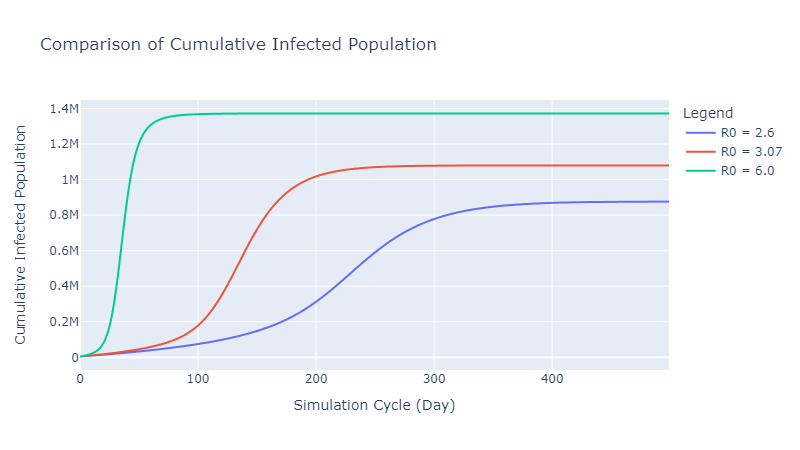
\includegraphics[width=0.95\textwidth]{Figures/InfectedR0.png}
  \caption{Simulations conducted with different basic reproduction ratios ($R_0$). The x-axis represents the simulation cycle (i.e., day), while the y-axis represents the cumulative infected population up to that point in the simulation.} 
  \label{fig:cumulative_infected}
\end{figure}
%python .\infection_sum_comparison.py --p infection_tests --e R0-2.6 R0-3.07 R0-6.0 --l "R0 = 2.6" "R0 = 3.07" "R0 = 6.0" --s 0 --x "Simulation Cycle (Day)" --y "Cumulative Infected Population"

For the remaining experiments, we will consider a baseline value of $R_0 = 2.6$ for the simulations. Figure~\ref{fig:sir_population_status} displays the total population amount for each possible value of the ``SIR Status" traceable characteristic over time in a simulation with $R_0 = 2.6$. It can be observed that despite reaching a cumulative infected population of 875,962 people (as shown in Figure~\ref{fig:cumulative_infected}), the peak of the infection occurred on day 247, with a total of 81,528 infected individuals at that point.

\begin{figure}[ht]
 \centering
  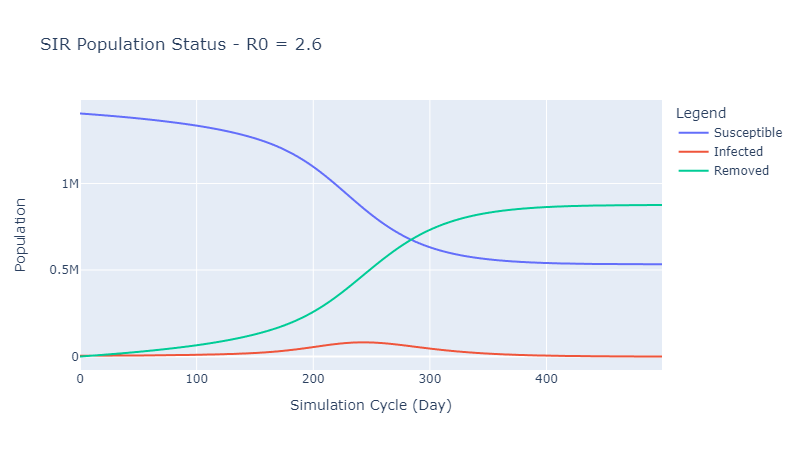
\includegraphics[width=0.95\textwidth]{Figures/SIRPopulationStatus.png}
  \caption{ Population count over time for each ``SIR Status" traceable property value in a simulation with $R_0 = 2.6$} 
  \label{fig:sir_population_status}
\end{figure}
%python .\experiment_global_population.py --p infection_tests --e R0-2.6 --c Susceptible Infected Removed --s 0 --x "Simulation Cycle (Day)" --t "SIR Population Status - R0 = 2.6"

Next, we extend the simulation to include additional behaviors related to epidemic contagion, specifically population vaccination as a measure to mitigate the spread of the disease. To facilitate this, we introduce a traceable characteristic called \textit{vaccine level} to all blobs in the simulation. This property is represented by an integer value. Additionally, we implement a new action called \textit{vaccinate}. When this action is triggered, a portion of the population is moved to a nearby ``pharmacy" $P$, which is available in all regions of the environment. At the pharmacies, the population receives a dose of the vaccine, resulting in an increase of their \textit{vaccine level} by 1. This signifies that they have been vaccinated and their resistance to the transmission of the virus has improved. Subsequently, the newly vaccinated population returns to their respective $P$s, such as workers returning to their ``work" $P$.

In our simulations, we explore various vaccination configurations by considering different dose counts, which represent the number of doses available to the population, as well as the effectiveness of each dose. Table~\ref{tbl:vaccine_configuration} summarizes the vaccination settings used in our experiments, where the Dose Count ranges from 1 to 3. The Effectiveness parameter indicates the efficacy of each dose in mitigating the spread of the infection.

All blobs in simulations with vaccinations contain a \textit{vaccine level} corresponding to an Effectiveness value in Table~\ref{tbl:vaccine_configuration}. Whenever a blob with \textit{SIR Status = Susceptible} gets infected, the amount of people that should be infected is defined by Equation~\ref{eq:deltaI}. The Effectiveness works by multiplying the result of Equation~\ref{eq:deltaI} by $1-Effectivess$, i.e., an $Effectivess=0.4$ reduces the amount of people changing from ``Susceptible" to ``Infected" by $40\%$. Starting Day indicates the simulation cycle at which each dose begins to be administered to the population. It is important to note that the second and third doses, if available, can only be administered to individuals who have already received the previous dose. Configurations A through C represent increasing effectiveness as more doses are administered, while Configuration D represents an ideal vaccine with 100\% effectiveness in preventing infection.

Building upon the parameters defined in previous experiments, all vaccination experiments utilize the routines of workers and students as the baseline, employing a scale parameter of $levy\_scale = 2$ and an \textit{infect} action with $R_0 = 2.6$. The global routine $GRo$ also includes the \textit{vaccinate} action, performed at selected cycle steps during the morning and afternoon of each day. To determine the number of individuals to be moved to ``pharmacy" $P$s on each simulation day, we gathered data on the daily number of COVID-19 vaccines administered in Porto Alegre\footnote{Dashboard of Brazilian vaccination data available \href{https://vacina.saude.rs.gov.br/}{HERE} (text in Brazilian Portuguese)}. This data is then proportionally distributed among the regions in the environment based on their respective populations.

\begin{table}[ht]
\centering
\caption{Configuration of vaccines for experiments. Dose Count represents the number of doses available for the population. Effectiveness represents how effective each dose is in reducing the spread of the infection. Starting Day represents the day (i.e., simulation cycle) when each dose starts being administered to the population. The second and third doses can only be applied to people who already received the previous dose. While VaccinationA, B, and C state for the doses, VaccinationD simulates a scenario where the effectiveness of the vaccine is 100\%.}
\label{tbl:vaccine_configuration}
\begin{tabular}{@{}lccc@{}}
\toprule
Vaccination Config & \multicolumn{1}{l}{Dose Count} & Effectiveness  & Starting Day  \\ \midrule
VaccinationA       & 1                              & {[}0.4{]}           & {[}50{]}           \\
VaccinationB       & 2                              & {[}0.4, 0.7{]}      & {[}50, 150{]}      \\
VaccinationC       & 3                              & {[}0.4, 0.7, 1.0{]} & {[}50, 150, 250{]} \\
VaccinationD       & 1                              & {[}1.0{]}           & {[}50{]}           \\ \bottomrule
\end{tabular}
\end{table}

Figure~\ref{fig:vaccines} showcases the results of the vaccination simulations. Despite the ``VaccinationA" configuration having an effectiveness of only 0.4, a significant impact on the cumulative infected population can be observed compared to the baseline. The baseline simulation resulted in a total of 875,962 infected individuals, whereas the ``VaccinationA" configuration achieved a notably lower count of 440,569 infected individuals. The incorporation of additional doses in the ``VaccinationB" and ``VaccinationC" configurations further decreased the cumulative infected population, resulting in 360,607 and 355,124 infected individuals, respectively. 
Although ``VaccinationC'' contains an effectiveness of $1.0$, this efficacy is only realized when the population undergoes the third dosage, initiated on day 250 of the simulation. Consequently, ``VaccinationB'' and ``VaccinationC'' are very similar until day 250, at which point the third dosage of ``VaccinationC'' begins to exert its influence, resulting in a small difference in the cumulative infected population of both simulations.
\red{Notably, the ``VaccinationD" configuration, representing an ideal vaccine, demonstrates the lowest number of infections, with only 170,978 individuals affected.}

\begin{figure}[ht]
 \centering
  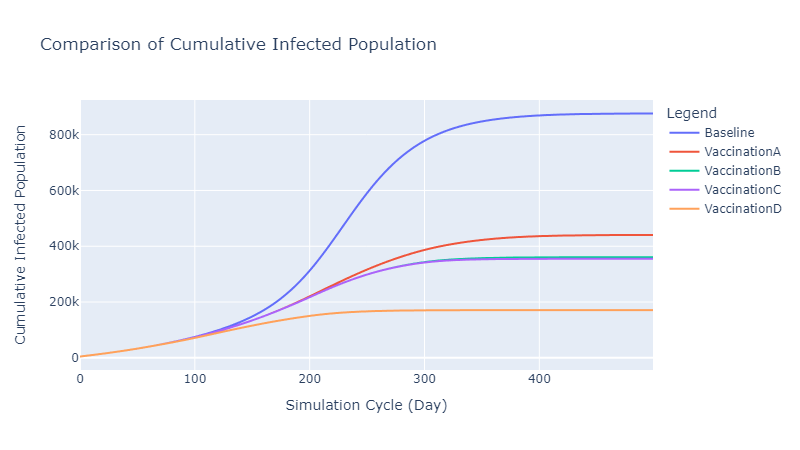
\includegraphics[width=0.95\textwidth]{Figures/InfectedVaccines.png}
  \caption{Simulations of different vaccination configurations, as described in Table~\ref{tbl:vaccine_configuration}. All simulations consider a basic reproduction rate of $R_0 = 2.6$.} 
  \label{fig:vaccines}
\end{figure}

\red{Finally, we explore the incorporation of movement restrictions in our epidemic contagion experiments to simulate lockdown behavior. The movement restriction is described in Section~\ref{sec:random_walk} and illustrated in Figure~\ref{fig7:movement_restriction}.} 
These experiments encompass a combination of three movement restriction values (no restriction, 0.5, and 0.75) that represent percentages of the population who do not leave their living neighborhoods, along with two vaccination scenarios: no vaccination; or ``VaccinationC", which includes three doses. 
We chose to compare the ``VaccinationC'' configuration rather than ``VaccinationD'' because ``VaccinationC'' exhibits a more realistic behavior. In ``VaccinationC'', the effectiveness of the vaccine increases with the number of doses a person receives. In contrast, ``VaccinationD'' represents an idealized vaccine with a fixed effectiveness of $1.0$ achieved in a single dose.

Figure~\ref{fig:vaccines_restrictions} illustrates the results obtained from our simulations. The imposition of movement restrictions reduces the cumulative infected population compared to the baseline scenario (no restriction and no vaccination). However, including population vaccination (experiment ``VaccC") exhibits more significant effectiveness in reducing the infected population compared to simulations with only movement restrictions. Moreover, the combination of movement restriction and vaccination demonstrates the most favorable outcomes, with the simulation containing a movement restriction of 0.75 and vaccination resulting in only 140,941 infected individuals.

%SO: an fig abaixo eu acharia legal comparar com vacin D que tu disseste antes que doi ideal
%GA: no caso trocar C por D ou também incluir D? Posso adicionar mas preciso pegar os resultados no lab, arquivos muito grandes pro git
\begin{figure}[ht]
 \centering
  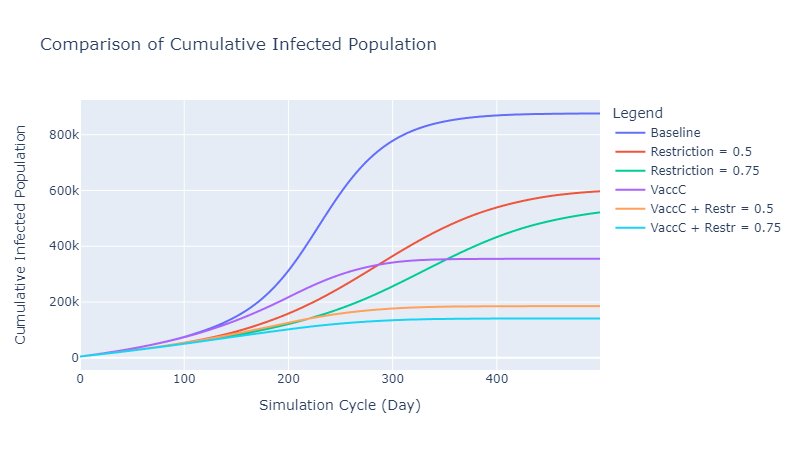
\includegraphics[width=0.95\textwidth]{Figures/InfectedVaccineRestriction.png}
  \caption{ Simulations of epidemic contagion. Experiments include a combination of three movement restriction values (no restriction, 0.5 and 0.75) to represent a lockdown and two vaccination scenarios (no vaccination or ``VaccinationC"). All simulations consider a basic reproduction rate of $R_0 = 2.6$.} 
  \label{fig:vaccines_restrictions}
\end{figure}


\subsection{Quantitative Performance Evaluation}
\label{sec:quant_perf}

\redc{To complement the qualitative case studies, we present a quantitative evaluation of LodusPop’s computational efficiency. All benchmarks use the Porto Alegre city model described in Section~\ref{sec:case_scenario} (94 regions, 504 points of interest, and a total population of $1,409,351$). Each configuration was executed five times, and average values are reported.

Table~\ref{tab:perf} reports quantitative information for each \textit{Case Study} and \textit{Configuration}, as follows: (i) \textit{Max Blob Count}, the maximum number of blobs observed during the run; (ii) \textit{Number of Cycles}, where a cycle corresponds to one simulated day in our setup, with 24 cycle steps; (iii) \textit{Avg Sim Time (s)}, the average total real-time required to complete the run; (iv) \textit{Time Per Cycle (s)}, the average runtime per simulated day; (v) \textit{MemProfile Avg Peak (MiB)}, the average peak resident memory of the Python process\footnote{Calculated with Memory Profiler v0.61.0: \url{https://pypi.org/project/memory-profiler/}}; and (vi) \textit{TraceMalloc Avg Peak (MiB)}, the average peak traced Python allocations\footnote{Calculated with TraceMalloc: \url{https://docs.python.org/3/library/tracemalloc.html}}. We interpret \textit{Max Blob Count} as an indicator of simulator workload: more frequent splits increase the number of population units to process and reduce merge opportunities, typically raising both runtime and memory consumption.

Using the random walk configuration of $levy\_scale=2$ (Section~\ref{sec:random_walk}) as the baseline simulation for the remaining case studies and configurations, the simulator completes a full run in $5.211s$ on average, with \emph{MemProfile Avg Peak} of $234.9$~MiB, and a \textit{TraceMalloc Avg Peak} of $58.565$~MiB. Introducing movement restrictions (Section~\ref{sec:random_walk}) slightly reduces \textit{Time Per Cycle} (down to $4.795s$ at $Restriction =0.75$), while peak memory remains essentially unchanged. This indicates that reduced mobility mainly decreases the number of executed move operations, without substantially changing blob splitting, as expected.

Large-scale events (Section~\ref{sec:large_scale}) increase runtime because they introduce additional gathering actions that relocate populations across distant locations. \textit{Time Per Cycle} rises from $6.144s$ (average simulations with one event) to $12.172s$ (simulation with four simultaneous events). These scenarios tend to produce fewer blobs, as populations aggregate around event locations, yet \textit{MemProfile Avg Peak} and \textit{TraceMalloc Avg Peak} remain close to the baseline ($\approx 235$~MiB and $\approx 59$~MiB, respectively). This indicates that the dominant cost comes from executing the large-scale gathering operations by pulling individuals from multiple regions and points of interest, rather than from an increase in blob count.

Epidemic contagion and vaccination simulations (Section~\ref{sec:contagion}) are more demanding because additional traceable characteristics (e.g., SIR status and vaccine level) increase population heterogeneity, causing more frequent splits and reducing merge opportunities. In our model, blobs can only merge when their traceable attributes match; as the simulation progresses, individuals become distributed across multiple states (susceptible, infected, removed) and vaccination levels, so blobs with different traceable characteristics cannot be merged back together.
For infection-only experiments, 500-cycle runs require $9.899$--$11.654s$ per cycle, and \textit{MemProfile Avg Peak} increases to roughly $1.72$--$1.80$~GiB. Vaccination scenarios further intensify splitting: VaccinationC reaches a \textit{Max Blob Count} of $23,355$ and requires $33.455s$ per cycle, with \textit{MemProfile Avg Peak} of $2.86$~GiB. Overall, \textit{Time Per Cycle} closely follows increases in \textit{Max Blob Count}, reinforcing that split and merge behaviors are key components of computational cost.

%Limitações das medidas
These measurements reflect the simulator execution on a single machine and are therefore hardware-dependent. The results are intended as a quantitative evaluation of the presented case studies, providing direct support for the efficiency and scalability claims within their scope, rather than as a head-to-head comparison with other simulation frameworks. 
All experiments were run on a machine with an AMD Ryzen 5 5600X CPU, an NVIDIA GeForce RTX 2060 GPU, 16GB DDR4 2666MHz (CL19) RAM, and a KINGSTON SNV3S1000G SSD, using Python v3.13.6 on Microsoft Windows 11 Education (Version 10.0.262000).}

\begin{table}[ht]
\redc{
\footnotesize
\centering
\caption{\redc{Quantitative performance evaluation of LodusPop. We use the Random Walk mobility configuration (Lévy-flight simulation with $levy\_scale=2$; Section~\ref{sec:random_walk}) as the baseline reference for the remaining case studies and configurations. For each case study and configuration, we report the maximum blob count observed during execution, the number of simulated cycles (days), the average total simulation time over five runs, the corresponding time per cycle, and peak memory usage measured via MemProfile (process RSS) and TraceMalloc (Python allocation tracing).}}
\label{tab:perf}
\begin{tabular}{@{}clllllll@{}}
\toprule
Case Study                                                                                                               & \multicolumn{1}{c}{Configuration} & \multicolumn{1}{c}{\begin{tabular}[c]{@{}c@{}}Max Blob\\ Count\end{tabular}} & \multicolumn{1}{c}{\begin{tabular}[c]{@{}c@{}}Number\\ of Cycles\end{tabular}} & \multicolumn{1}{c}{\begin{tabular}[c]{@{}c@{}}Avg Sim\\ Time (s)\end{tabular}} & \multicolumn{1}{c}{\begin{tabular}[c]{@{}c@{}}Time Per\\ Cycle (s)\end{tabular}} & \multicolumn{1}{c}{\begin{tabular}[c]{@{}c@{}}MemProfile\\ Avg Peak\\ (MiB)\end{tabular}} & \multicolumn{1}{c}{\begin{tabular}[c]{@{}c@{}}TraceMalloc\\ Avg Peak\\ (MiB)\end{tabular}} \\ \midrule
\begin{tabular}[c]{@{}c@{}}Baseline\\ (Random Walk)\\Case Study 1\end{tabular}                                                                                                                & $levy\_scale = 2$                          & 2857                                                                         & 1                                                                              & 5.211                                                                          & 5.211                                                                            & 234.912                                                                                 & 58.565                                                                                   \\ \midrule
\multirow{3}{*}{\begin{tabular}[c]{@{}c@{}}Movement \\Restriction (Fig~\ref{fig7:movement_restriction})\\Case Study 1\end{tabular}}                                         & Restriction = 0.25                & 2871                                                                         & 1                                                                              & 5.074                                                                          & 5.074                                                                            & 234.957                                                                                 & 58.577                                                                                   \\
                                                                                                                       & Restriction = 0.50                & 2864                                                                         & 1                                                                              & 4.958                                                                          & 4.958                                                                            & 234.935                                                                                 & 58.527                                                                                   \\
                                                                                                                       & Restriction = 0.75                & 2883                                                                         & 1                                                                              & 4.795                                                                          & 4.795                                                                            & 235.234                                                                                 & 58.516                                                                                   \\ \midrule
\multirow{5}{*}{\begin{tabular}[c]{@{}c@{}}Large-Scale Events\\ (Fig~\ref{fig8:results_displacements} and Table~\ref{tbl:results_displacement})\\Case Study 2\end{tabular}}                                 & Average of 1 Event                & 2671                                                                         & 1                                                                              & 6.144                                                                          & 6.144                                                                            & 235.355                                                                                 & 58.767                                                                                   \\
                                                                                                                       & Average of 2 Events               & 2651                                                                         & 1                                                                              & 7.986                                                                          & 7.986                                                                            & 235.297                                                                                 & 58.892                                                                                   \\
                                                                                                                       & Average of 3 Events               & 2651                                                                         & 1                                                                              & 9.910                                                                          & 9.910                                                                            & 235.530                                                                                 & 59.061                                                                                   \\
                                                                                                                       & 4 Events                          & 2651                                                                         & 1                                                                              & 12.172                                                                         & 12.172                                                                           & 235.825                                                                                 & 59.217                                                                                   \\
                                                                                                                       & 4 Events at Different Times       & 2079                                                                         & 1                                                                              & 11.153                                                                         & 11.153                                                                           & 235.355                                                                                 & 59.146                                                                                   \\ \midrule
\multirow{3}{*}{\begin{tabular}[c]{@{}c@{}}Infection (Fig~\ref{fig:cumulative_infected})\\Case Study 3\end{tabular}}                                          & $R_0$ = 2.6                          & 8840                                                                         & 500                                                                            & 5826.840                                                                       & 11.654                                                                           & 1798.114                                                                                & 1554.886                                                                                 \\
                                                                                                                       & $R_0$ = 3.07                         & 8830                                                                         & 500                                                                            & 5630.155                                                                       & 11.260                                                                           & 1741.606                                                                                & 1520.793                                                                                 \\
                                                                                                                       & $R_0$ = 6.0                          & 8818                                                                         & 500                                                                            & 4949.313                                                                       & 9.899                                                                            & 1718.252                                                                                & 1480.354                                                                                 \\ \midrule
\multirow{4}{*}{\begin{tabular}[c]{@{}c@{}}Vaccination\\ (Fig~\ref{fig:vaccines} and Table~\ref{tbl:vaccine_configuration})\\Case Study 3\end{tabular}}                                        & VaccA                             & 16495                                                                        & 500                                                                            & 8991.828                                                                       & 17.984                                                                           & 2246.849                                                                                & 2057.299                                                                                 \\
                                                                                                                       & VaccB                             & 20840                                                                        & 500                                                                            & 11346.181                                                                      & 22.692                                                                           & 2250.278                                                                                & 2318.228                                                                                 \\
                                                                                                                       & VaccC                             & 23355                                                                        & 500                                                                            & 16727.571                                                                      & 33.455                                                                           & 2862.153                                                                                & 2512.703                                                                                 \\
                                                                                                                       & VaccD                             & 12542                                                                        & 500                                                                            & 7620.026                                                                       & 15.240                                                                           & 1750.923                                                                                & 1883.745                                                                                 \\ \midrule
\multirow{4}{*}{\begin{tabular}[c]{@{}c@{}}Vaccination and\\Restriction (Fig~\ref{fig:vaccines_restrictions})\\Case Study 3\end{tabular}} & $R_0$ = 2.6; Restriction = 0.50      & 9011                                                                         & 500                                                                            & 4008.347                                                                       & 8.017                                                                            & 1983.816                                                                                & 1743.626                                                                                 \\
                                                                                                                       & $R_0$ = 2.6; Restriction = 0.75      & 8320                                                                         & 500                                                                            & 4566.876                                                                       & 9.134                                                                            & 1681.857                                                                                & 1472.081                                                                                 \\
                                                                                                                       & VaccC; Restriction = 0.50         & 16722                                                                        & 500                                                                            & 9279.227                                                                       & 18.558                                                                           & 2628.414                                                                                & 2313.595                                                                                 \\
                                                                                                                       & VaccC; Restriction = 0.75         & 15429                                                                        & 500                                                                            & 8139.657                                                                       & 16.279                                                                           & 2540.851                                                                                & 2240.514                                                                                 \\ \bottomrule
\end{tabular}
} %  end of redc
\end{table}

\subsection{Comments about Multi-resolution Environments}
\label{sec:comments}


Several points are worth noting when discussing multi-resolution environments. First, in our Case-Scenario (Section~\ref{sec:case_scenario}), we defined the points of interest ($P$s) as being associated with specific locations within the city of Porto Alegre; consequently, the population motion occurred in the city, with populations moving between $P$s.
However, the spatial scope of these $P$s can be adjusted to suit the needs of simulation designers or specific experiments.
For instance, these $P$s could represent locations in various cities within a state, and distances between cities could then be calculated, enabling the application of navigation models such as Levy walk or alternative movement algorithms. Movement restrictions could also be modeled, as demonstrated in Figure~\ref{fig7:movement_restriction}. 
Similarly, large-scale events (Section~\ref{sec:large_scale}) could be simulated where individuals travel from one city to another, or regions could be conceptualized as states within a country. This flexibility highlights the adaptability of our population simulation model to operate with different spatial abstractions.
Regarding the epidemic contagion scenarios presented in Section~\ref{sec:contagion}, parameters related to contagion dynamics may require adjustments to reflect larger distances between individuals, such as when simulating interactions across different states. This capability underscores the framework's scalability and the potential for extending its use to broader contexts.

Finally, our simulation results are effectively visualized within multi-level simulation environments, offering insights into population dynamics across different spatial scales.
Figure~\ref{fig:multi_level_visualization} illustrates population movements, highlighting interactions between spatial levels.
Figure~\ref{fig:visualization_region} provides a detailed view of the city environment, incorporating additional visual elements such as roads and buildings to contextualize the simulations. In these visualizations, the red area represents a designated $P$ in the simulation, acting as a focal point for population activities.
Figure~\ref{fig:visualization_blob} demonstrates populations moving between multiple $P$s, showcasing the framework’s ability to model and track mobility across multiple regions. The visualization was developed using Unity.

\begin{figure}[!htb]
  \centering
  \subfloat[\red{A detailed representation of the city with roads and buildings. The highlighted red area represents a designated $P$ in the environment.}]
  {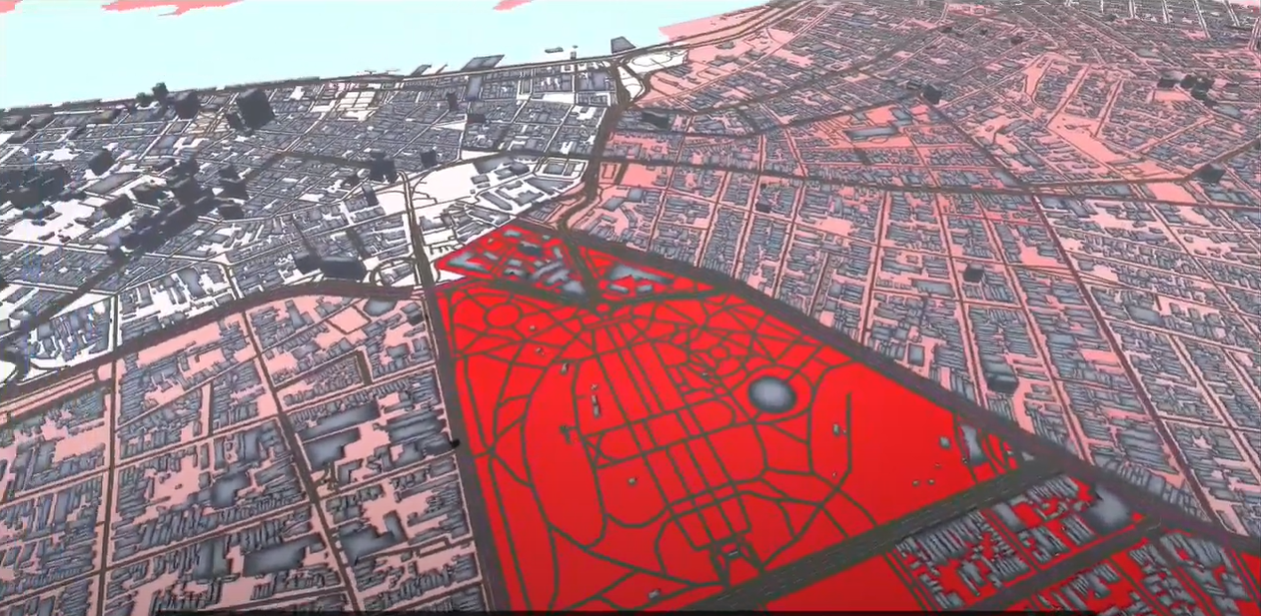
\includegraphics[width=0.95\textwidth]{Figures/Lodus1.png}
  \label{fig:visualization_region}}\\
  \subfloat[\red{Visualization of populations moving between multiple $P$s in the environment.}]
  {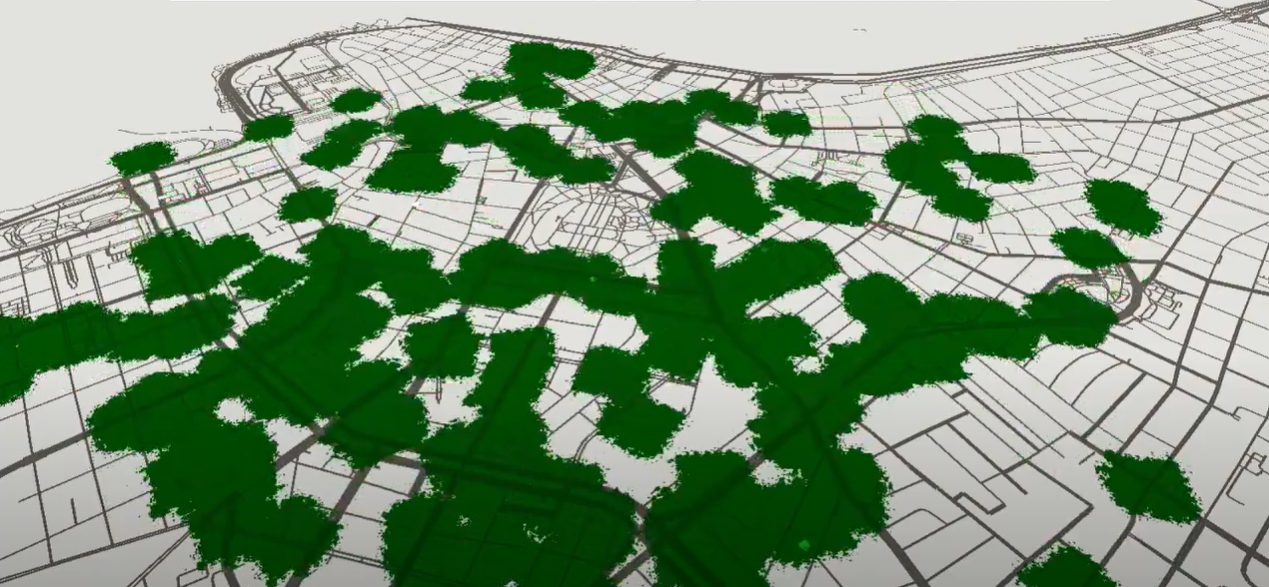
\includegraphics[width=0.95\textwidth]{Figures/Lodus2.png}
  \label{fig:visualization_blob}}
  \caption{\red{Visualization of our simulations in a multi-level environment. (a) present a detailed visualization of the city, and (b) presents the abstract population moving between different $P$s in the environment.}}
  \label{fig:multi_level_visualization}
\end{figure}

\section{Final Considerations} 
\label{sec:final_considerations}

This work introduced LodusPop, a flexible framework for simulating urban population dynamics across multiple spatial and temporal scales. 
\redb{By combining an environment-driven paradigm with blob abstractions, LodusPop enables the representation of population dynamics at multiple spatial and temporal scales while reducing reliance on fine-grained individual data.}
%By combining an environment-driven paradigm with the blob abstractions, LodusPop enables the representation of both macro- and micro-level behaviors while reducing reliance on fine-grained individual data. 
This makes it particularly suited to contexts where privacy concerns or limited data availability constrain traditional population-driven approaches.

Our experiments demonstrated the framework’s versatility in addressing diverse real-world challenges, ranging from everyday mobility and large-scale events to epidemic contagion and vaccination strategies. These case studies highlight how LodusPop can capture both short-term disruptions and long-term dynamics, underscoring its potential for practical applications in urban planning, public health, disaster management, and crisis response. Importantly, the extensible plugin architecture and JSON-based input design ensure that new action types, data sources, and policies can be integrated with minimal effort, making LodusPop adaptable to different research and policy contexts.

Despite these contributions, some limitations remain. The level of detail in simulations is directly tied to the granularity of available data, often constrained by census or municipal surveys. Current assumptions—such as independence among sampled characteristics—may oversimplify correlations between attributes like age, occupation, or mobility patterns. Addressing these limitations will require integrating dynamic data sources and statistical dependencies, which would further enhance realism and adaptability.
%Aqui
\redc{Our evaluation reports quantitative runtime and memory measurements for the presented case studies on a single machine; therefore, the results are hardware- and case-dependent and are intended to characterize scalability trends in our implementation rather than provide head-to-head benchmarking against other frameworks.}
%
Moreover, the current implementation operates exclusively with environment-driven blob dynamics; integrating explicit agent-based micro-dynamics via the plugin interface is an important avenue for future work.
We also leave as priorities for future work a formal complexity analysis, richer evaluation metrics, and comparative studies against real mobility data.
Future research may also explore validation strategies based on synthetic datasets, interoperability with urban digital twin platforms, and coupling with machine learning methods to generate adaptive, data-driven behaviors.

Evaluating LodusPop against state-of-the-art models remains challenging, as existing frameworks like MATSim~\citep{balmer2009matsim}, SUMO~\citep{krajzewicz2012sumo}, and GAMA~\citep{taillandier2019gama} either require detailed travel demand data, focus narrowly on traffic, or depend on explicit behavioral rules. In contrast, LodusPop offers a complementary perspective: less data-hungry than traffic simulators, more adaptable than statistical mobility models, and uniquely capable of supporting rapid policy evaluation in heterogeneous and low-data environments.

In summary, LodusPop establishes a robust foundation for simulating complex and evolving population dynamics. Its design and extensibility position it as a bridge between research and practice, providing researchers, planners, and policymakers with a powerful tool for evidence-based decision-making in domains as diverse as population mobility, crisis management, and sustainable urban development.

\begin{comment}
    

This work introduced LodusPop, a model for simulating population dynamics in diverse environments. LodusPop enables the representation of both macro- and micro-level behaviors, allowing researchers to explore the intricate interactions between populations and their environments. By considering population characteristics and extensible plugins, our model offers a flexible approach to simulating scenarios ranging from everyday mobility patterns to large-scale events that disrupts daily routines and public health crises.

The experiments demonstrated the framework's ability to address various real-world challenges. From simulating random walk behaviors and large-scale events to modeling the spread of infectious diseases and the impact of vaccination strategies, the results highlighted the versatility of LodusPop in capturing both short-term and long-term population dynamics. One of our main contributions, the capability to represent populations as abstract blobs of varying sizes, underscore the potential for practical applications in urban planning and public health.

% Limitations and future work
Despite its contributions, the current implementation of LodusPop has limitations. The granularity of input data, for instance, directly impacts the level of detail that can be modeled in the simulations. While the framework supports highly detailed configurations, the availability of granular data often depends on external sources, such as census and municipal surveys. 
Furthermore, certain assumptions, like fixed distributions for population characteristics, may require refinement to better suit specific applications or more complex scenarios.
Another limitation lies in the representation of sampled characteristics, which currently assumes independence among different attributes. This approach does not account for potential joint distributions or correlations between these characteristics, which could improve the realism and accuracy of the simulations. 
Future research could focus on integrating dynamic data sources to enhance real-time adaptability and refining our proposed model to incorporate more sophisticated statistical dependencies of for population characteristics. These improvements would further strengthen LodusPop's utility in modeling diverse and evolving scenarios.

Evaluating our proposed methodology against state-of-the-art models poses a considerable challenge, as, to the best of our knowledge, there are no existing simulation models with sufficiently comparable features to enable a meaningful and relevant comparison. Traditional population-driven crowd simulation models in the literature typically focus on simulating individual agents or groups based on predefined behaviors~\citep{cao2021competitiveCooperative, zhang2023collectiveBehavior, antonitsch2019bioclouds}. While these models excel at capturing detailed population-level dynamics, they often struggle with scalability and require extensive, high-quality datasets to calibrate individual or group behaviors. 
In contrast, our environment-driven approach focuses on the demands of the environment rather than individual agents or groups. This perspective enables modeling interactions between populations and their environments across varying scales. 
Additionally, validating the simulation using real-world data presents inherent difficulties. Privacy regulations impose significant restrictions on the collection and use of detailed mobility data, while data from governmental agencies, when available, often lack the granularity or completeness required for robust validation. Unlike many existing models that rely on specific datasets or scenarios, our framework is designed to operate with varying levels of data availability, making it adaptable to a range of contexts where comprehensive data may be inaccessible.

%Evaluating our proposed methodology against state-of-the-art models poses a considerable challenge, as, to the best of our knowledge, there are no existing simulation models with sufficiently comparable features to enable a meaningful and relevant comparison. Additionally, validating the simulation using real-world data is inherently difficult. The collection of such data, particularly for mobility-related scenarios, is hindered by strict privacy regulations and the limited accessibility of data from governmental agencies.

LodusPop provides a robust foundation for simulating complex population dynamics, offering valuable insights for researchers and policymakers. Its design and extensibility ensure that our model can be adapted to a wide range of use cases, making it a powerful tool for addressing challenges in population mobility, public health, and resource allocation.
\end{comment}





\backmatter

\begin{comment}
\bmhead{Supplementary information}

If your article has accompanying supplementary file/s please state so here. 

Authors reporting data from electrophoretic gels and blots should supply the full unprocessed scans for key as part of their Supplementary information. This may be requested by the editorial team/s if it is missing.

Please refer to Journal-level guidance for any specific requirements.
\end{comment}

\bmhead{Acknowledgements}

% Esta no funding
%This study was partly financed by the Coordenação de Aperfeiçoamento de Pessoal de Nivel Superior – Brasil (CAPES) – Finance Code 001, and by the Conselho Nacional de Desenvolvimento Científico e Tecnológico - Brasil (CNPq) - Process Number 309228/2021-2.

The authors acknowledge the use of ChatGPT, version GPT-4o, to review and enhance the text quality of this paper, ensuring clarity and coherence in its presentation.
    
\section*{Declarations}

%Some journals require declarations to be submitted in a standardised format. Please check the Instructions for Authors of the journal to which you are submitting to see if you need to complete this section. If yes, your manuscript must contain the following sections under the heading `Declarations':

\bmhead{Funding}
This study was partly funded by: the Coordenação de Aperfeiçoamento de Pessoal de Nivel Superior – Brasil (CAPES) – Finance Code 001; the Conselho Nacional de Desenvolvimento Científico e Tecnológico - Brasil (CNPq) - Process Number 309228/2021-2; the Fundação de Amparo à Pesquisa do Estado do Rio Grande do Sul (FAPERGS) - Process Number 20/2551-0000280-2; and the Instituto Nacional de Ciência e Tecnologia em
Simulação e Monitoramento para Assistência ao
Indivíduo em Eventos Climáticos Extremos (INCT-SiM-AI) - Process Number 408330/2024-4.

\bmhead{Competing Interests}
The authors declare that they have no known competing financial interests or personal relationships that could have appeared to
influence the work reported in this paper

\bmhead{Data availability}
Data will be made available on request.

\bmhead{Code availability}
Code will be made available on request.

\bmhead{Author contribution}
\textbf{Gabriel Fonseca Silva:} Conceptualization, Methodology, Software, Validation, Investigation, Writing – original draft, Writing – review \& editing, Visualization. \textbf{André da Silva Antonitsch}: Conceptualization, Methodology, Investigation. \textbf{Soraia Raupp Musse:} Conceptualization, Methodology, Validation, Investigation, Writing – review \& editing, Supervision, Project administration, Funding acquisition.

\begin{appendices}

\section{Input and Simulation Setup}
\label{app:input}

This Appendix provides examples of the data input and simulation setup required to execute simulations, as defined by our proposed model in Section~\ref{sec:proposed_model}. The setup includes:
\begin{itemize}
    \item \textit{i)} input files describing the environment, population, and routines (detailed in Appendices~\ref{app:input_environment},~\ref{app:input_population} and ~\ref{app:input_routine}, respectively);
    \item \textit{ii)} plugin scripts to introduce new action types into the simulation (Appendix~\ref{app:plugin}); and
    \item \textit{iii)} a simulator script responsible for executing the simulation.
\end{itemize}
In the current implementation, both the simulator and plugin scripts are written in Python, and the input data is structured in the JSON file format, ensuring ease of use and extensibility.


\subsection{Environment Input Files}
\label{app:input_environment}
\red{The environment input file provides a detailed description of all regions ($R$s) and their respective points of interest ($P$s) in the simulation, in accordance with the definitions outlined in Section~\ref{sec:environment}. Listing~\ref{lst:environment_description} illustrates an example environment configuration containing a single region named \textit{``ExampleRegion''}, which includes three points of interest: a school, a pharmacy, and a home. Data to describe the environment can be obtained from Geographic Information System (GIS) databases such as OpenStreetMap, as presented in Figure~\ref{fig:data_diagram}.

Each element in the environment input file, whether a region or a point of interest, is characterized by an identifier and a geographical location. These attributes are specified using the \textit{name} and \textit{lng\_lat} properties, respectively.}

\begin{lstlisting}[language={python},
caption={Example of an environment input file.},
captionpos=b, label={lst:environment_description}, basicstyle=\footnotesize]
"regions": [ 
  {
    "name": "ExampleRegion",
    "lng_lat": [-51.19757, -30.15647],
    "points_of_interest": [
      { 
        "name": "school",
        "lng_lat": [-51.19750, -30.15621]
      },
      { 
        "name": "pharmacy",
        "lng_lat": [-51.19820, -30.15655]
      },
      { 
        "name": "home",
        "lng_lat": [-51.19805, -30.15633]
      }
    ]
  } 
]
\end{lstlisting}

\subsection{Population Input Files}
\label{app:input_population}

The population input file provides a detailed description of all blobs ($B$s), including their characteristics and locations at the start of the simulation, in alignment with the definitions in Section~\ref{sec:population}. Listing~\ref{lst:population_description} presents an example population input containing two initial blobs. Population data can be sourced from census data (Real Population) or generated synthetically (Synthetic Population) to meet the specific requirements of an experiment, as shown in Figure~\ref{fig:data_diagram}.

The \textit{default\_traceable\_characteristics} property sets default values for the $\bm{Tc}$s of all blobs. Unless explicitly defined in their setup, all blobs start the simulation with a \textit{VaccinationStatus} traceable characteristic set to \textit{Unvaccinated}.

The \textit{sampled\_characteristics\_categories} property specifies the possible categories for each sampled characteristic used by all blobs in the simulation. However, the population distribution across these categories is defined individually for each blob, as described below.

The \textit{initial\_population} property outlines points of interest and their initial populations (i.e., $\bm{B}_{P}$). Points of interest are identified by their containing regions and identifiers, such as \textit{"ExampleRegion//home"}, which references the \textit{home} $P$ within \textit{ExampleRegion}, as described in Listing~\ref{lst:environment_description}. A point of interest may include multiple blob descriptions, but only those with an initial population need to be included in the input file.

Each $P$ within \textit{initial\_population} contains a vector of elements describing blobs, with each element providing:
\begin{itemize}
    \item The total population of a blob ($TP$);
    \item Optional values for $\bm{Tc}$, which override the \textit{default\_traceable\_characteristics}; and
    \item Values for all categories of the $\bm{Sc}$. 
\end{itemize}  
For instance, in Listing~\ref{lst:population_description}, two blobs are created in the \textit{home} $P$ of \textit{ExampleRegion}. Blob $B_i$ has $TP_i = 100$, with its $\bm{Tc}_i$ equal to the default values, as no specific values were assigned in its \textit{"traceable\_characteristics"} property. Blob $B_j$, on the other hand, has $TP_j = 20$ and an initial \textit{VaccinationStatus} traceable characteristic value of \textit{Vaccinated}.

\begin{lstlisting}[language={Python},
caption={Example of a population input file.},
captionpos=b, label={lst:population_description}, basicstyle=\footnotesize]
"default_traceable_characteristics": {
  "VaccinationStatus": "Unvaccinated",
  "Traceable_B": "Value_B"
},
"sampled_characteristics_categories": {
  "Age": ["Children", "Adults", "Elders"],
  "Sampled_B": ["Value_B1", "Value_B2"]
},
"initial_population": {
  "ExampleRegion//home": [
    {
      "total_population": 100,
      "traceable_characteristics": {},
      "sampled_characteristics": {
          "Age": { "Children": 20, "Adults": 50, "Elders": 30 },
          "Sampled_B": { "Value_B1": 43, "Value_B2": 57 }
      }
    },
    {
      "total_population": 20,
      "traceable_characteristics": {
        "VaccinationStatus": "Vaccinated"
      },
      "sampled_characteristics": {
          "Age": { "Children": 20, "Adults": 0, "Elders": 0 },
          "Sampled_B": { "Value_B1": 12, "Value_B2": 8 }
      }
    }
  ]
}
\end{lstlisting}

\subsection{Routine Input Files}
\label{app:input_routine}

The routine input file provides a description of the Global Routine ($GRo$) and the local routines for individual points of interest, following the definitions outlined in Section~\ref{sec:routines}. Listing~\ref{lst:routine_description} presents an example input containing routines for two points of interest: a \textit{home} $P_i$ and a \textit{pharmacy} $P_j$, both located in the \textit{ExampleRegion}.

$P_i$ includes a single action, $A_i$, executed at $t = 8$ during each simulation cycle. $A_i$ is of type \textit{move population} (defined in Section~\ref{sec:routines}) and moves 20 individuals—specifically unvaccinated children and young students—from $P_i$ to the \textit{pharmacy} $P_j$ in \textit{ExampleRegion}.

$P_j$, on the other hand, has two actions, $A_j$ and $A_k$, performed at $t = 9$ and $t = 10$, respectively, during each simulation cycle. $A_j$ is of type \textit{change traceable characteristic} (detailed in Section~\ref{sec:routines}), vaccinating 5 people currently at $P_j$. $A_k$, of type \textit{move population}, transfers the vaccinated individuals from $P_j$ back to $P_i$.

The \textit{population\_template} property specifies the profile of individuals selected for each action, such as students who are children or young adults. The \textit{name} property, included as a label, does not influence the simulation directly but serves as a reference for annotating the purpose of the action.
While Listing~\ref{lst:routine_description} does not include actions for the Global Routine, these follow the same structure as individual routines, encompassing a cycle step, action type, population template, and any additional parameters.


\begin{lstlisting}[language={Python},
caption={Example of a routine input file.},
captionpos=b, label={lst:routine_description}, basicstyle=\tiny]
"global_routine": [],
"routines": {
  "ExampleRegion//home": [
    {
      "cycle_step": 8,
      "action": {
        "name": "send_students_to_pharmacy",
        "type": "move_population",
        "population_template": {
          "traceable_characteristics": {
             "VaccinationStatus": "Unvaccinated"
          },
          "sampled_characteristics": {
            "Age": [ "Children", "Youngs" ],
            "Occupation": [ "Student" ]
          }
        },
        "values": {
          "origin_region": "ExampleRegion",
          "origin_poi": "home",
          "destination_region": "ExampleRegion",
          "destination_poi": "pharmacy",
          "quantity": 20
        }
      }
    }
  ],
  "ExampleRegion//pharmacy": [
    {
      "cycle_step": 9,
      "action": {
        "name": "vaccinate_population",
        "type": "change_traceable_characteristic",
        "population_template": {
          "traceable_characteristics": {
            "VaccinationStatus": "Unvaccinated"
          },
          "sampled_characteristics": {}
        },
        "values": {
          "characteristic_to_change": "VaccinationStatus",
          "new_value": "Vaccinated",
          "quantity": 5
        }
      }
    },
    {
      "cycle_step": 10,
      "action": {
        "name": "send_vaccinated_population_back",
        "type": "move_population",
        "population_template": {
          "traceable_characteristics": {
            "VaccinationStatus": "Vaccinated"
          },
          "sampled_characteristics": {}
        },
        "values": {
          "origin_region": "ExampleRegion",
          "origin_poi": "pharmacy",
          "destination_region": "ExampleRegion",
          "destination_poi": "home",
          "quantity": 5
        }
      }
    }
  ]
}
\end{lstlisting}

\subsection{Plugins}
\label{app:plugin}
Plugins define additional action types and their corresponding functions while also providing external parameters and data. These resources enable simulation designers to tailor simulations and model diverse scenarios. Plugins are implemented as Python modules and imported by the simulator script, described in the following section. 

Listing~\ref{lst:plugin_script} shows an example plugin that processes the \textit{"example\_action"} action type. This action transfers 100 individuals from a point of interest $P_i$, specified by the \textit{values} parameter, to a \textit{home} $P_j$ within the same region. The plugin accomplishes this by creating and returning a \textit{move population} action, which is then executed by its corresponding function.


\begin{lstlisting}[language={Python},
caption={Example of a plugin script that includes a "example\_action" in the simulation.},
captionpos=b, label={lst:plugin_script}, basicstyle=\footnotesize]
class ExamplePlugin(environment.TimeActionPlugin):

    def __init__(self, environment_graph):
        super().__init__()
        self.graph = environment_graph
        self.set_pair('example_action', self.consume_action)
        self.example_external_parameter = 'foo'

    def consume_action(self, pop_template, values, cycle_step, sim_step):
        region = self.graph.get_region(values['region'])
        poi = region.get_poi(values['node'])

        new_action_type = 'move_population'
        new_action_values = {}
        new_action_values['origin_region'] = region.name
        new_action_values['origin_poi'] = poi.name
        new_action_values['destination_region'] = region.name
        new_action_values['destination_poi'] = 'home'
        new_action_values['quantity'] = 100
        action = environment.TimeAction(_type = new_action_type,
                                        _pop_template = pop_template,
                                        _values = new_action_values)
        return [action]
\end{lstlisting}

\subsection{Simulator script}
\label{app:simulator}

The simulator script manages the parsing of input data, the integration of plugins, and the overall control of the simulation flow. 
Listing~\ref{lst:simulator} presents an example of a simulator script. Parsing is handled by a function that takes input file paths as arguments and returns an \textit{EnvGraph} framework class instance.
Plugins are incorporated by initializing their classes and loading them into the \textit{EnvGraph}. The simulation flow is governed by a loop that updates the simulation step at each iteration.


\begin{lstlisting}[caption={Simulation script example.},captionpos=b, label={lst:simulator}, basicstyle=\footnotesize, language=Python]
# Data Loading
env_graph = Generate_EnvironmentGraph([data_input_file_paths])

# Simulation Parameters
cycles = 3
cycle_duration = 24
env_graph.routine_cycle_length = cycle_duration
simulation_steps = cycles * cycle_duration

# Loading Plugins
ex_pluging = ExamplePlugin(env_graph)
ex_pluging.example_external_parameter = 'bar'
env_graph.LoadPlugin(ex_pluging)

# SIMULATION
for i in range(simulation_steps):
  # Updates POI Routines and Global Routines
  # These are defined by the input files
  env_graph.update_time_step(i % cycle_duration, I)
  
  # Actions can be directly called or queued in the simulation loop
  # if i == 60:
  #   dummy_action = TimeAction(_type = new_action_type,
  #                             _pop_template = dummy_template,
  #                             _values = dummy_values)
  #   env_graph.direct_action_invoke(dummy_action)
  #   env_graph.queue_next_frame_action(dummy_action)
\end{lstlisting}

%%=============================================%%
%% For submissions to Nature Portfolio Journals %%
%% please use the heading ``Extended Data''.   %%
%%=============================================%%

%%=============================================================%%
%% Sample for another appendix section			       %%
%%=============================================================%%

%% \section{Example of another appendix section}\label{secA2}%
%% Appendices may be used for helpful, supporting or essential material that would otherwise 
%% clutter, break up or be distracting to the text. Appendices can consist of sections, figures, 
%% tables and equations etc.


\end{appendices}

%%===========================================================================================%%
%% If you are submitting to one of the Nature Portfolio journals, using the eJP submission   %%
%% system, please include the references within the manuscript file itself. You may do this  %%
%% by copying the reference list from your .bbl file, paste it into the main manuscript .tex %%
%% file, and delete the associated \verb+\bibliography+ commands.                            %%
%%===========================================================================================%%

\bibliography{bib}% common bib file
%% if required, the content of .bbl file can be included here once bbl is generated
%%\input sn-article.bbl

\end{document}
